%%%%%%%%%%%%%%%%%%%%%%%%%%%%%%%%%%%%%%%%%
% Short Sectioned Assignment
% LaTeX Template
% Version 1.0 (5/5/12)
%
% This template has been downloaded from:
% http://www.LaTeXTemplates.com
%
% Original author:
% Frits Wenneker (http://www.howtotex.com)
%
% License:
% CC BY-NC-SA 3.0 (http://creativecommons.org/licenses/by-nc-sa/3.0/)
%
%%%%%%%%%%%%%%%%%%%%%%%%%%%%%%%%%%%%%%%%%
%----------------------------------------------------------------------------------------
%	PACKAGES AND OTHER DOCUMENT CONFIGURATIONS
%----------------------------------------------------------------------------------------
\documentclass[paper=a4, fontsize=12pt, liststotoc,bibtotoc]{scrartcl} % A4 paper and 11pt font size
\usepackage[utf8]{inputenc}
\usepackage[T1]{fontenc} % Use 8-bit encoding that has 256 glyphs
\usepackage{fourier} % Use the Adobe Utopia font for the document - comment this line to return to the LaTeX default
\usepackage[german]{babel} % German language/hyphenation
\usepackage{amsmath,amsfonts,amsthm} % Math packages
\usepackage{color}
\definecolor{gruen}{rgb}{0,0.5,0}
\definecolor{blau}{rgb}{0,0,1}
\definecolor{lila}{rgb}{0.4,0.1,0.5}
\definecolor{darkblue}{rgb}{0,0,0.5}
\definecolor{grau}{rgb}{0.5,0.5,0.5}
\definecolor{schwarz}{rgb}{0,0,0}
\definecolor{magentat}{rgb}{0.88,0,0.45}
\definecolor{gelbt}{rgb}{0.98,0.76,0.40}
\definecolor{gruent}{rgb}{0.73,0.74,0.35}
\definecolor{dunkelblaut}{rgb}{0.26,0.48,0.67}
\definecolor{grau01t}{rgb}{0.64,0.64,0.64}

\usepackage{listings}
\lstdefinelanguage{XML}{
morestring=[s]{"}{"},
identifierstyle=\color{blue},
stringstyle=\color{gruen},
basicstyle=\ttfamily\footnotesize,
emph={android},
emphstyle=\color{lila},
moredelim=[s][\color{darkblue}]{<}{\ },
moredelim=[s][\color{darkblue}]{</}{>},
moredelim=[l][\color{darkblue}]{/>},
moredelim=[l][\color{darkblue}]{>},
belowcaptionskip=1\baselineskip,
breaklines=true,
showstringspaces=false,
xleftmargin=\parindent
}

\lstdefinelanguage{JAVA}{
morekeywords={public, class, long, return, int, private, import, final, extends, static, if, else, null, void, super, while, new, boolean, protected, default, switch, break, try, catch, for, package, true, mark},
keywordstyle=\bfseries\color{darkblue},
morestring=[s]{"}{"},
commentstyle =\itshape\color{grau},
identifierstyle=\color{schwarz},
stringstyle=\color{gruen},
basicstyle=\footnotesize\ttfamily,
emph={inflater, tv_date, tv_name, context, name, namelist_name, tv_mark, magenta, gruen, gelb, tv_semester, GONE, TERMINDETAIL, notenList, semesterList, fachList, versuchList, newsResolver, intent, datum, tv_category, grau01, dunkelblau, kategorie, tv1, tv2, tv3, tv4, ladebalken, tv_news_date, tv_news_hl1, tv_news_hl2, tv_news_content, doc},
emphstyle=\color{lila},
belowcaptionskip=1\baselineskip,
breaklines=true,
showstringspaces=false,
xleftmargin=\parindent,
frame=single,
moredelim=[is][\textcolor{blau}]{\%\%}{\%\%},
moredelim=[is][\itshape\textcolor{grau}]{$$}{$$},
}



\usepackage[colorlinks,linkcolor=darkblue,citecolor=red,urlcolor=blue]{hyperref}
\usepackage{titlesec}

\usepackage{sectsty} % Allows customizing section commands
\allsectionsfont{\centering \normalfont\scshape} % Make all sections centered, the default font and small caps
\usepackage{fancyhdr} % Custom headers and footers
\pagestyle{fancyplain} % Makes all pages in the document conform to the custom headers and footers
%\fancyhead{T} % No page header - if you want one, create it in the same way as the footers below
\fancyhead[L]{HFTL-APP}
\fancyhead[C]{}
\fancyhead[R]{Projektarbeit Software-Engineering}
\fancyfoot[L]{} % Empty left footer
\fancyfoot[C]{BKMI 13} % Empty center footer
\fancyfoot[R]{\thepage} % Page numbering for right footer
\renewcommand{\headrulewidth}{1pt} % Remove header underlines
\renewcommand{\footrulewidth}{1pt} % Remove footer underlines
\setlength{\headheight}{13.6pt} % Customize the height of the header
\setlength{\footheight}{8mm}
\numberwithin{equation}{section} % Number equations within sections (i.e. 1.1, 1.2, 2.1, 2.2 instead of 1, 2, 3, 4)
\numberwithin{figure}{section} % Number figures within sections (i.e. 1.1, 1.2, 2.1, 2.2 instead of 1, 2, 3, 4)
\numberwithin{table}{section} % Number tables within sections (i.e. 1.1, 1.2, 2.1, 2.2 instead of 1, 2, 3, 4)
\setlength\parindent{0pt} % Removes all indentation from paragraphs - comment this line for an assignment with lots of text


\newcommand{\horrule}[1]{\rule{\linewidth}{#1}} % Create horizontal rule command with 1 argument of height

\author{BKMI 13} % Your name

\date{\normalsize\today} % Today's date or a custom date
\bibliographystyle{unsrt}

%%%%%%%%%%%eigene Sachen%%%%%%%%%%%%%%%%%%%%%%%%%%%%
\flushbottom 
\usepackage{graphicx}
\usepackage{microtype}    
% Abkürzungsverzeichniss
\usepackage[printonlyused]{acronym}
\usepackage{wrapfig}
% Inhaltsverzeichnis auch in Time New Roman
\addtokomafont{sectioning}{\rmfamily}
\usepackage[section]{placeins}
\usepackage{pdflscape}		%Seiten teilweise auf Querformat drehen
\usepackage[final]{pdfpages} 		%Einfügen von bestehenden .pdf Seitem
  
\setcounter{secnumdepth}{4} %damit im Dokument tiefer gegliedert wird
\setcounter{tocdepth}{4}	%damit im Inhaltsverzeichnis tiefer gegliedert wird


%%%%%%%%%%%%%%%%%%%%%%%%TEST%%%%%%%%%%%
%			Erstellung Klasse SUBSUBSUBSECTION zur tieferen Verschachtelung der Gliederung, da sonst bei Subsubsection Ende ist  %%%%%%%%%

%%%%      \bfseries   für FETTDRUCK in DEKLARATION          %%%%%



\titleclass{\subsubsubsection}{straight}[\subsection]

\newcounter{subsubsubsection}[subsubsection]
\renewcommand\thesubsubsubsection{\thesubsubsection.\arabic{subsubsubsection}}
\renewcommand\theparagraph{\thesubsubsubsection.\arabic{paragraph}} % optional; useful if paragraphs are to be numbered

\titleformat{\subsubsubsection}
  {\centering\normalsize}{\thesubsubsubsection}{1em}{}
\titlespacing*{\subsubsubsection}
{0pt}{3.25ex plus 1ex minus .2ex}{1.5ex plus .2ex}

\makeatletter
\renewcommand\paragraph{\@startsection{paragraph}{5}{\z@}%
  {3.25ex \@plus1ex \@minus.2ex}%
  {-1em}%
  {\normalfont\normalsize\bfseries}}
\renewcommand\subparagraph{\@startsection{subparagraph}{6}{\parindent}%
  {3.25ex \@plus1ex \@minus .2ex}%
  {-1em}%
  {\normalfont\normalsize\bfseries}}
\def\toclevel@subsubsubsection{4}
\def\toclevel@paragraph{5}
\def\toclevel@paragraph{6}
\def\l@subsubsubsection{\@dottedtocline{4}{7em}{4em}}
\def\l@paragraph{\@dottedtocline{5}{10em}{5em}}
\def\l@subparagraph{\@dottedtocline{6}{14em}{6em}}
\makeatother







%%%%%%%%%%%%%%%%%%%%%%%%%%%%%%%%%%%%%%%%%%%%%%%%%%%%%%%%%%
%%%%%%%%%%%%%%%%%%%%%%%%%%%%%%%%%%%%%%%%%%%%%%%%%%%%%%%%%%
%%%%%%%%%	Begin des eigentlichen Dokuments  %%%%%%%%%%%%
%%%%%%%%%%%%%%%%%%%%%%%%%%%%%%%%%%%%%%%%%%%%%%%%%%%%%%%%%%
%%%%%%%%%%%%%%%%%%%%%%%%%%%%%%%%%%%%%%%%%%%%%%%%%%%%%%%%%%


\begin{document}

\pagestyle{empty}
%\maketitle % Print the title
\begin{center}
\begin{tabular}{p{\textwidth}}


\begin{center}
\includegraphics[scale=0.5]{img/HFTL-Logo.pdf}
\end{center}


\\

\begin{center}
\LARGE{\textsc{
Entwicklung einer HFTL-APP \\
Dokumentation\\
}}
\end{center}

\\


\begin{center}
\large{Studienmodul \textit{Software-Engineering} \\
der Hochschule für Telekommunikation\\
Leipzig\\}
\end{center}

\\

\begin{center}
\textbf{\Large{Projektarbeit - Softwareentwicklung}}
\end{center}


%\begin{center}
%zur Erlangung des akademischen Grades\\
%Bachelor of Engineering
%\end{center}


\begin{center}
vorgelegt von
\end{center}

\begin{center}
\large{\textbf{BKMI Matrikel 13}} \\
\small{}
\end{center}

\begin{center}
\large{23.04.2015}
\end{center}

\\

\\

\begin{center}
\begin{tabular}{lll}
\textbf{Dozent:} & & Profn. Dr.-Ing. Sabine Wieland\\
%\textbf{Zweitprüfer:} & &Prof. Dr.-Ing. F. Musterfrau\\
\end{tabular}
\end{center}

\end{tabular}
\end{center}
%\part im Inhaltsverzeichnis nicht nummerieren
\makeatletter
\let\partbackup\l@part
\renewcommand*\l@part[2]{\partbackup{#1}{}}

\newpage

%Seitennummerierung neu beginnen, Zahlen [arabic], röm.Zahlen [roman,Roman], Buchstaben [alph,Alph]
\pagenumbering{arabic}

\cleardoublepage\pdfbookmark{Inhaltsverzeichnis}{toc} %Inhaltsverzeichnis im PDF

\tableofcontents
%\listoffigures
\pagestyle{fancy}
\newpage

% \section{Software Requirements Specification}

\section{Einführung}

\subsection{\textbf{Zweck}}
Dieses Dokument dient als Grundlage zur Beauftragung des berufsbegleitenden Studienganges, Kommunikations- und Medieninformatik des Matrikel 13, mit der Programmierung einer \acs{HfTL}-\acs{APP}. Es setzt dabei die Rahmenbedingungen fest.

\subsection{\textbf{Hintergründe und Ziele des Projekts}}
Die \acf{HfTL} ist eine private, staatlich anerkannte Fachhochschule. Träger der \ac{HfTL} ist die \ac{HfTL}-Trägergesellschaft \acs{mbH}, eine Beteiligungsgesellschaft der Deutschen Telekom AG. Die Schule befindet sich im Leipziger Stadtteil Connewitz. Es werden sowohl Direkt- als auch duale Studiengänge und berufsbegleitende Studiengänge angeboten.
Aufgrund des umständlichen Beschaffens der Noten und Stundenpläne sowie der Termine für Teletutorings, wird eine Smartphone-Applikation benötigt. Diese stellt ein Benutzerinterface für Studenten der \acs{HfTL} dar, mit dem der Zugriff auf die im \acs{QIS} hinterlegten Daten vereinfacht.

\subsection{\textbf{Produktumfang}}

Der Betrieb der \acs{HfTL}-APP muss auf allen gängigen Android-Smartphones ab Version 4.0 möglich sein.

Durch die APP wird den Studenten der HFTL ermöglicht: 

\begin{itemize}
      \item die aktuellsten Nachrichten der \acs{HfTL}-Webseite lesen
      \item auf \acs{QIS} zugreifen
      \item Studenten sollen ihre(-n) Noten(-spiegel) aufrufen können
      \item Vorlesungspläne zu lesen
      \item Raumbelegungspläne abzurufen
\end{itemize}
   
Zusätzlich werden folgende Anforderungen gestellt:

\begin{itemize}
	\item Erweiterbarkeit für weitere Funktionen und Anwender
	\item spätere IOS-Version
\end{itemize}


\subsection{\textbf{Musskriterien}}

Zunächst müssen zwingend folgende Punkte des Umfangs erfüllt werden:

\begin{itemize}
   	\item NEWS
   	\item NOTEN
   	\item STUNDENPLAN   
\end{itemize}

\subsection{\textbf{Abgrenzungskriterien}}

Die \acs{APP} soll später auch für zusätzliche Informationen, wie ein Raumplanung erweiterbar sein. Eine spätere Version für IOS-Geräte ist ebenfalls geplant, ist hier aber nicht Bestandteil.				

\subsubsection{Kostenrahmen}

Für die Entwicklung der \acs{APP} soll auf kostenfreie Opensource-Programme oder auf vordefinierte Klassen der Programmierung zurückgegriffen werden.
Außer den personellen Aufwand dürfen keine Zusätzlichen Kosten entstehen.


\subsection{\textbf{Definitionen, Akronyme, Abkürzungen}}
\begin{acronym}[UV-Licht]
\acro{HfTL}{Hochschule für Kommunikation Leipzig}
\acro{APP}{Kurzform für Applikation}
\acro{mbH}{mit beschränkter Haftung}
\acro{QIS}{Qualitätssteigerung der Hochschulverwaltung im Internet durch Selbstbedienung}
\acro{iCal}{Datenformat zum Austausch von Kalenderinhalten}
\acro{SoSe15}{Sommersemester 2015}
\acro{XML}{ Extensible Markup Language}
\acro{HTTPS}{HyperText Transfer Protocol Secure}
\acro{AES}{Advanced Encryption Standard}
\acro{SQL}{Structured Query Language}
\acro{.apk}{Android application package}
\acro{MTBF}{mean time between failure}

\end{acronym}

\subsection{\textbf{Referenzen}}

\begin{itemize}		
	\item QIS-System:  \url{https://qisweb.hispro.de/tel/rds?state=user&type=0} 
	
	\item News der HfTL  \url{https://www.hft-leipzig.de/de/studierende/service/news.html}	
\end{itemize}


\section{Allgemeine Übersicht}

\subsection{\textbf{Beschreibung der Ausgangssituation (Ist-Zustand) }}

Damit Studenten auf \acs{QIS} zugreifen kann, müssen diese sich über einen Browser auf der \acs{QIS}-Seite einloggen und über das unübersichtliche Menü ihre Daten suchen.
Studenten haben die Möglichkeit ihre Noten oder einen Notenspiegel einzusehen.
Für IPhone-Nutzer gibt es bereits eine kostenpflichtige \acs{APP} , namens Grades, die Noten und Informationen über die angemeldete Prüfungen auslesen kann.
Um die auf \acs{QIS} hinterlegten Vorlesungspläne abzurufen ist kein Login erforderlich, jedoch ist es notwendig sich umständlich zu dem entsprechenden Studiengang zu navigieren. Einzelne Vorlesungen oder Stundenpläne können als \acs{iCal} heruntergeladen werden.
Ebenso sind die Teletutorien hier zu finden.
Die aktuellen Nachrichten der Hochschul-Homepage sind auf einer anderen Seite zu finden, welche öffentlich zugänglich ist.


\subsection{\textbf{Produkteinsatz}}

\subsubsection{Anwendungsbereiche}
Aktuell soll die APP nur für die Studenten der \acs{HfTL} zugänglich sein, welche ein Android-Smartphone besitzen. 

\subsubsection{Zielgruppen, Qualifikationsniveau}

Da bei der Nutzergruppe von Studenten mit Erfahrung im Umgang mit solchen APP's ausgegangen werden kann, wird auch die Oberfläche dementsprechend gestaltet.

\subsection{\textbf{Produktfunktionalität}}

Die APP soll sich mittels regelmäßiger Abfragen der \acs{HfTL}-Homepage, sowie von \acs{QIS}, die News, Noten und Stunden- und ggf. Raumbelegungspläne ziehen und die Noten für den Nutzer lokal auf dem Smartphone speichern und entsprechend darstellen. 
Es soll sichergestellt werden das auf sensible Daten wie z.B. Noten auch nur autorisierte Nutzer Zugang bekommen. Die APP soll in deutscher Sprache dargestellt werden. Evtl. wird sie im Nachgang in andere Sprachen übersetzt. 

\subsection{\textbf{Randbedingungen}}

Der zeitliche Rahmen für die Entwicklung und Programmierung dieser APP begrenzt sich auf das \ac{SoSe15} und dem Studienmodul Software-Engineering.
Für die Entwicklung dieser APP, sowie Vertrieb, Programmierung usw. dürfen keine Kosten entstehen.
Supportleistungen werden in der Projektphase über das Projektteam geleistet. Die Wartung wird, bis mit der Veröffentlichung die APP der Hochschule kostenfrei zur Verfügung gestellt wird, ebenfalls vom Projektteam übernommen. Die Dokumentation wird ebenfalls vollständig an die Hochschule übergeben.
Durch das Projektteam wird es keine weitere Softwarebetreuung, Wartung oder der gleichen geben. Es finden ebenfalls keine Schulungen oder Einweisungen statt.

\subsection{\textbf{Annahmen und Abhängigkeiten}}

Die APP wird für Android-Geräte ab Version 4.0.3 zur Verfügung stehen.
Entsprechend der Vorgaben der Deutschen Telekom AG muss bei der Programmierung der APP, explizit beim Design, auf die Konzernrichtlinien geachtet werden. Es soll zusätzlich auf die Designempfehlungen für Androidgeräte geachtet werden.

\subsection{\textbf{Verzögerungen}}

Durch die strikte Abtrennung des zeitlichen Rahmens auf das \acs{SoSe15} darf es über diesen Zeitraum hinaus nicht zu Verzögerungen kommen

\section{Anwendungsszenarien}

\subsection{\textbf{Beschreibung aus der Nutzersicht}}

Die Benutzeroberfläche muss intuitiv bedienbar sein. Der strukturierte Aufbau durch Kategorien (News, Noten, Stundenplan) soll die Übersichtlichkeit erhöhen.
Die Logindaten werden verschlüsselt auf dem Smartphone gespeichert und auch verschlüsselt übertragen.
Durch eine durchgehende und vollständige Dokumentation soll eine Wartung auch durch spätere Matrikel oder Administratoren der Hochschule möglich sein.
Eine Implementierung weiterer Funktionen soll auch im Nachhinein möglich sein.

\section{Anforderungen}

\subsection{\textbf{Fachkonzept}}
Die \acs{HfTL}-APP  wird in Java programmiert um durch Verwendung bestehender Klassen die Erweiterbarkeit und Realisierbarkeit zu vereinfachen. Für das Design werden \acs{XML}-Stylesheets verwendet.
Pull-und Push-Service werden zur Benachrichtigung und Abfrage verwendet.




\subsubsection{Überblick über das Gesamtsystem}
$\;$ \\ %Zeilenumbruch bei Nutzung von paragraph

\textbf{Noten}
\begin{itemize}
	\item die APP soll die Noten lokal auf dem Smartphone nach Semester aufgeschlüsselt anzeigen
	\item Login über die APP
	\item Anmeldung über gesicherte, verschlüsselte Übertragung (\acs{HTTPS})
	\item verschlüsselte Speicherung der Daten auf dem Smartphone (\acs{AES})
	\item verschlüsselte Speicherung der Daten auf dem Smartphone (\acs{AES})
	\item Pull-Nachrichten (Einstellbares Intervall und/oder manuell)
	\item Push-Benachrichtigung
	\item Nutzer wird mit Hinweismeldung informiert, wenn Noten aktualisiert wurden
\end{itemize}
Optionale Angaben im Menüpunkt Noten:
\begin{itemize}
	\item Klassenspiegel
	\item Notenverteilung
	\item Anzahl der Teilnehmer
	\item Notenschnitt
	\item Anzeige der Creditpoints
	\item zu erreichende Creditpoints
	\item erreichte Creditpoints
\end{itemize}
\textbf{Stundenpläne}
\begin{itemize}
	\item Stundenplan nur für zum Nutzer passenden Studiengang
	\item Pull-Nachrichten (Einstellbares Intervall und/oder manuelle Abfrage)
	\item Synchronisierung mit dem Kalender auf dem Smartphone	
\end{itemize}
\textbf{News}
\begin{itemize}
	\item Pull-Nachrichten (manuelle Aktualisierung)
	\item News von: \url{https://www.hft-leipzig.de/de/studierende/service/news.html}
\end{itemize}



\subsubsection{Verwendete Bibliotheken von Drittanbieteren}
\begin{itemize}
	\item jsoup 1.8.1 – MIT-Lizenz
	\item iCal4j 1.0.6 – BSD-Lizenz 
\end{itemize}


\subsection{\textbf{Anforderungen an die Datenhaltung}}

Alle gespeicherten Daten müssen vor unbefugtem Zugriff geschützt werden, dafür werden Benutzerdaten in einer \acs{SQL}-Datenbank gespeichert und durch das Passwort und den Benutzernamen freigegeben. Passwort und Benutzername wurden mit \acs{AES} verschlüsselt.

\subsubsection{allgemeine Beschreibung der Daten}
Sicherheitsrelevante Daten sind in dem Notenteil der App zu finden. Diese sind der Benutzername, das Passwort, die Prüfungs- und Prüfungsvorleistungsergebnisse, der Klassenspiegel und die Creditpoints.
Die öffentlichen Daten sind in den anderen beiden Teilen der App enthalten.
Dazu gehören die News mit ihren Terminen und Inhalt und der Stundenplan mit den Veranstaltungen und den dazugehörenden Informationen wie Dozent und Veranstaltungsort.


\subsection{\textbf{Anforderungen an die Benutzeroberfläche}}



\subsubsection{allgemeine Anforderungen an die Oberfläche}
\textcolor{magenta}{kommt noch von MAIK/Stefan}




\subsubsection{Berechtigungen}

Die APP wird als Open Source bereitgestellt.

Nicht angemeldete Benutzer können sich die News und den Stundenplan anzeigen lassen. Angemeldete Benutzer können zusätzlich ihre Noten abrufen.

Die App braucht folgende Berechtigung auf dem Smartphone:
\begin{itemize}
	\item Netzwerkstatus abrufen: zur Kontrolle ob das Handy online ist
	\item Internet: APP greift auf das Internet zu
	\item Telefonstatus: wird zur Verschlüsselung benötigt
\end{itemize}




\subsubsection{Bildschirmlayout}
\textcolor{magenta}{Layouterklärung von Maik/Stefan}





\subsubsection{Dialogstruktur, Dialogabläufe}
\textcolor{magenta}{Maik/Stefan bitte hier Screenshots der jeweiligen Dialoge einfügen oder in Anhang unter Dialogmasken}





\subsection{\textbf{Leistungsanforderungen}}
Es wird von einer maximalen Nutzerzahl von 1000 Studenten ausgegangen.
Die Reaktionszeit/Programmstart der APP soll möglichst gering gehalten werden.
Das Datenaufkommen soll möglichst gering ausfallen.


\subsection{\textbf{Anfordeungen für Inbetriebnahme und Einsatz}}

\subsubsection{Sicherheitsziele}
Der Benutzername und das Passwort werden in einen gesicherten Speicherbereich (nur root), mit \acs{AES} verschlüsselt, gespeichert.
Die Datenbank in der die Noten gespeichert werden, liegt ebenfalls in diesem Bereich und darf nur von der \acs{HfTL}-App geöffnet werden.
Die Kommunikation mit der \acs{HfTL}-Website und \acs{QIS} erfolgt gesichert per \acs{HTTPS}.



\subsubsection{Installationsprozedur}

Der Wirkbetrieb soll nach Möglichkeit über den Android-Playstore realisiert werden. Falls es dabei zu Lizenz- und Kostenproblemen kommt, wird die APP als \ac{.apk} über die HfTL-Homepage verteilt.



\subsubsection{Pilot- bzw. Probebetrieb}
\textcolor{magenta}{Hier müssen die Versionsmanagementprotokolle rein!}




\subsubsection{Fehlerreaktion, Garantie, Service, »Wiederanlauf«}
Die Zuverlässigkeit sollte sich durch eine große \ac{MTBF} darstellen.



\subsubsection{Schulungen}
Nach Beendigung des Projektes werden keine Schulungen usw. durchgeführt.


\subsection{\textbf{Qualitätsanforderungen}}

\subsubsection{Qualitätsmerkmale}
Folgende Qualitätsansprüche werden gestellt:
\begin{itemize}
	\item Hohe Zuverlässigkeit der Software
	\item schnelle und zuverlässige Verarbeitung der gewünschten Daten
	\item sichere Datenspeicherung u. -übertragung mittels entsprechender Verschlüsselung
	\item Fehler werden mit einer entsprechenden Fehlermeldung beantwortet
	\item Intuitiv benutzbar
	\item Leicht zu warten und zu erweitern
	\item Vollständige Dokumentation des Projektes
\end{itemize}




\subsubsection{Qualitätssicherung}
Zur Qualitätssicherung werden einheitliche Testprotokolle und die entsprechenden Testkriterien erstellt. Es finden regelmäßige Kontrollen durch die Qualitätssicherung statt, um die Einhaltung der gegebenen Standards zu überprüfen. Es findet ebenfalls eine regelmäßige Kontrolle der Dokumentation statt. Die jeweiligen Software-Prototypen werden nach der Prototypisierung zur Fehlererkennung und zum Funktionstest an das Projektteam geschickt. Zur Verbesserung der Software werden die Tests anhand vorgegebener Testkriterien durchgeführt, um standardisierte Testergebnisse zu erhalten. Die Testergebnisse werden zur Auswertung an die entsprechende Projektgruppen zurück gespiegelt.


\subsubsection{Qualitätsnachweise}
Während des Projektzeitraumes werden sämtliche Meeting, Tests und Kontrollen protokolliert und zur Dokumentation in einem dafür vorgesehen Bereich abgelegt. Die gesetzten Standards und Vorgaben werden eingehalten. Zum Projektabschluss ist der geplante Umfang erreicht und alle Muss-Kriterien sind enthalten. Die APP ist funktionstüchtig.



\subsubsection{Offenlegung der Qualitätskontrollpläne}
\textcolor{magenta}{Hat Patrick da was zu???}



\subsubsection{Berichte, Protokolle zum Nachweis des Vorgehens gemäß der Qualitätskontrollpläne}
Es liegen bei:
\begin{itemize}
	\item Sitzungsprotokolle etc. (siehe Anlagen)
\end{itemize}



\subsection{\textbf{Anforderung an die Entwicklung}}

\subsubsection{Entwicklungs-Umgebung}
Für die Entwicklung wird Android Studio inkl. Gradle in der Version 1.x genutzt. Für die Dokumentation und Projektkoordination wird GitHub verwendet.



\subsubsection{Projekt-Organisation}
\textcolor{magenta}{Verweis auf Projektorganigramm im Anhang}


\subsubsection{Projekt-Planung}
\textcolor{magenta}{Verweis auf Projektstrukturplan im Anhang}

\subsubsection{Änderungsmanagement}
\textcolor{magenta}{GitHub Plan????}

\subsubsection{Testanforderungen}
\textcolor{magenta}{Testprotokollentwurf}



\section{Anhang}

\textcolor{magenta}{
\begin{itemize}
	\item Dialogmasken
	\item Dokumente
	\item Liste der Softwarelieferungen
	\item Projektorganigramm
	\item Projektstrukturplan
	\item Haupt-Termindaten
\end{itemize}
}
\newpage
\begin{figure}[h]
	\centering
	
\includegraphics[scale=2.5]{03_Bedienungsanleitung/img/Logo_HFTl_App.png}
	\label{img:grafik-dummy}
\end{figure}

\begin{center}
{\huge Benutzerhandbuch}
\end{center}


\newpage
\section{Benutzerhandbuch}
\subsection{Funktionsumfang}
In diesem Dokument wird die Benutzerfunktionen von der HfTL-APP für
Android-Geräte beschrieben. Es dient als Benutzerhandbuch für die
unterschiedlichen Funktionen der Anwendung und soll Ihnen beim
Ausführen von häufigen Aktionen innerhalb der Anwendung Hilfe bieten.
Die Installation und Konfiguration von der HfTL-APP wird in einem
separaten Dokument behandelt.

Die HfTL-APP ist eine mobile Informationslösung für Android Geräte. Die App kann kostenlos über das Rechenzentrum der Hochschule für Kommunikation-Leipzig bezogen werden.

Die HfTL-APP bietet folgende Funktionen:

\begin{itemize}
\item Abfrage der News von der HfTL-Homepage
\item Abfrage der Noten aus QIS/HIS nach erfolgreicher Anmeldung an dem betreffenden System
\item Abfrage des zu einem Studenten passenden Stundenplans
\end{itemize}

HINWEIS: In diesem Dokument wird vorausgesetzt, dass die HfTL-APP bereits installiert ist.
\begin{figure}[h]
	\centering
	\includegraphics[scale=0.5]{03_Bedienungsanleitung/img/appstore.jpg}
	%\caption{eine Grafik ohne Sinn und Verstand}
	\label{img:grafik-dummy}
\end{figure}

\newpage

\subsection{Startbildschirm}


\begin{figure}[h]
	\centering
	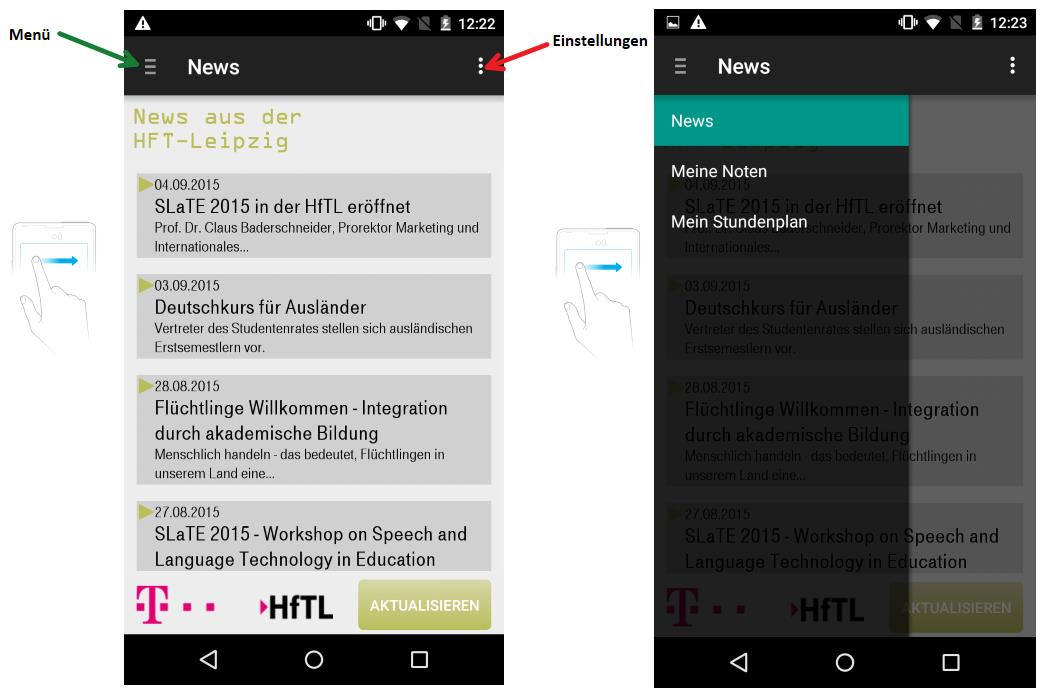
\includegraphics[scale=0.8]{03_Bedienungsanleitung/img/start2.jpg}
	%\caption{eine Grafik ohne Sinn und Verstand}
	\label{img:grafik-dummy}
\end{figure}

%\begin{wrapfigure}{r}{0.5\textwidth}
  %\begin{center}
   % 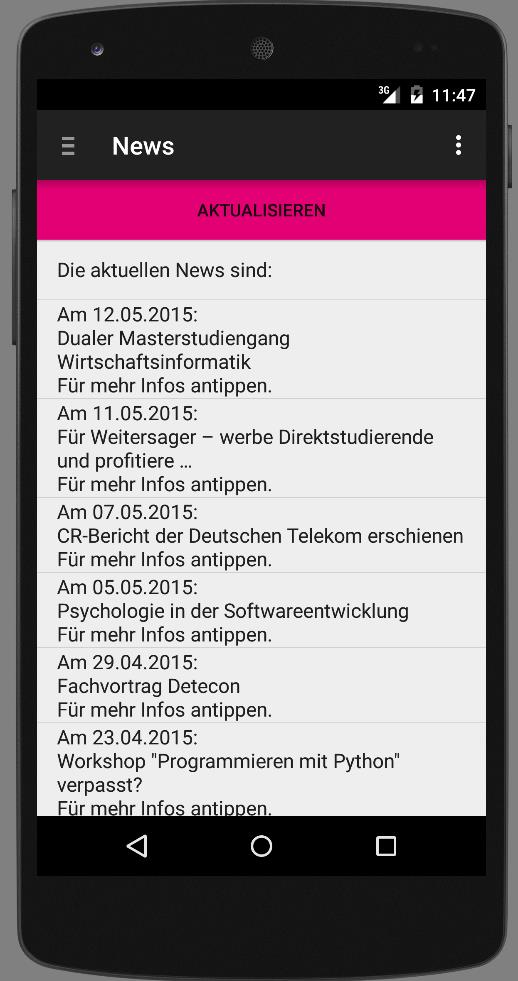
\includegraphics[width=0.5\textwidth]{03_Bedienungsanleitung/img/start.jpg}
  %\end{center}
  %\caption{HFTL-APP©gemeinfrei}
 % \label{reaper}
%\end{wrapfigure}

Nach Starten der APP erscheint zunächst die News-Seite. Die News werden bei bestehender Internetverbindung automatisch aktualisiert. Mit klicken auf den Aktualisierungsbutton kann eine manuelle Aktualisierung durch den Nutzer angestoßen werden.

Über den Menü-Button gelangt der Nutzer in das Programm-Menü. Über den Einstellungs-Button gelangt man in das Einstellungs-Menü.
Mit Auswählen der einzelnen News gelangt man in deren Detailansicht.

\newpage
\subsection{Newsansicht}
\begin{figure}[h]
	\centering
	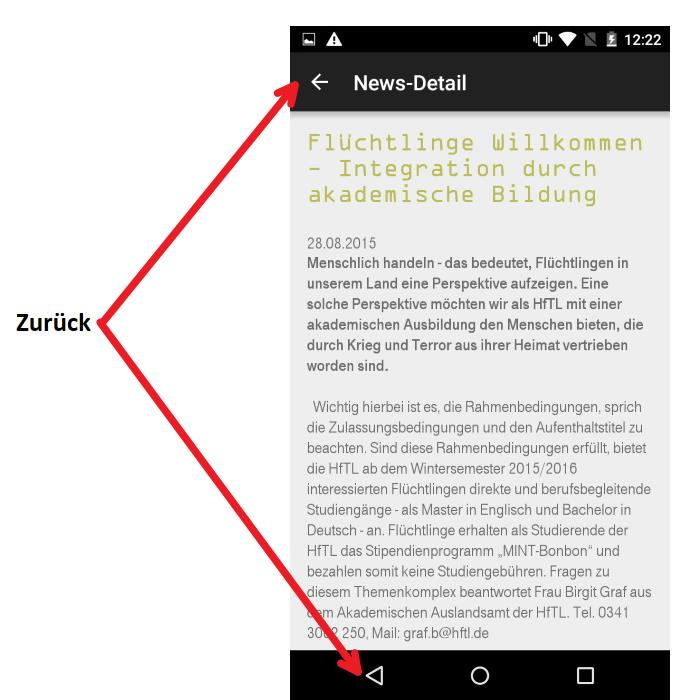
\includegraphics[scale=0.8]{03_Bedienungsanleitung/img/news.jpg}
	%\caption{eine Grafik ohne Sinn und Verstand}
	\label{img:grafik-dummy}
\end{figure}

Mit den Zurück-Buttons gelangt man in die vorherige Ansicht.

\newpage
\subsection{Noten}

Um die Noten abzurufen geht man zunächst in den Einstellungskontext. Dort kann der Nutzer und das jeweilige Passwort eingegeben werden.
\\
\\
Mit einem Klick auf Benutzername bzw. Passwort öffnet sich ein neuer Kontext welcher zum eingeben des Benutzernamens bzw. Passwortes auffordert.
\\
\\
Nach Eintippen kann der Kontext mit "OK" gespeichert und verlassen werden.

\begin{figure}[htb]
    \centering
    \begin{minipage}{0.45\linewidth}
        \centering
        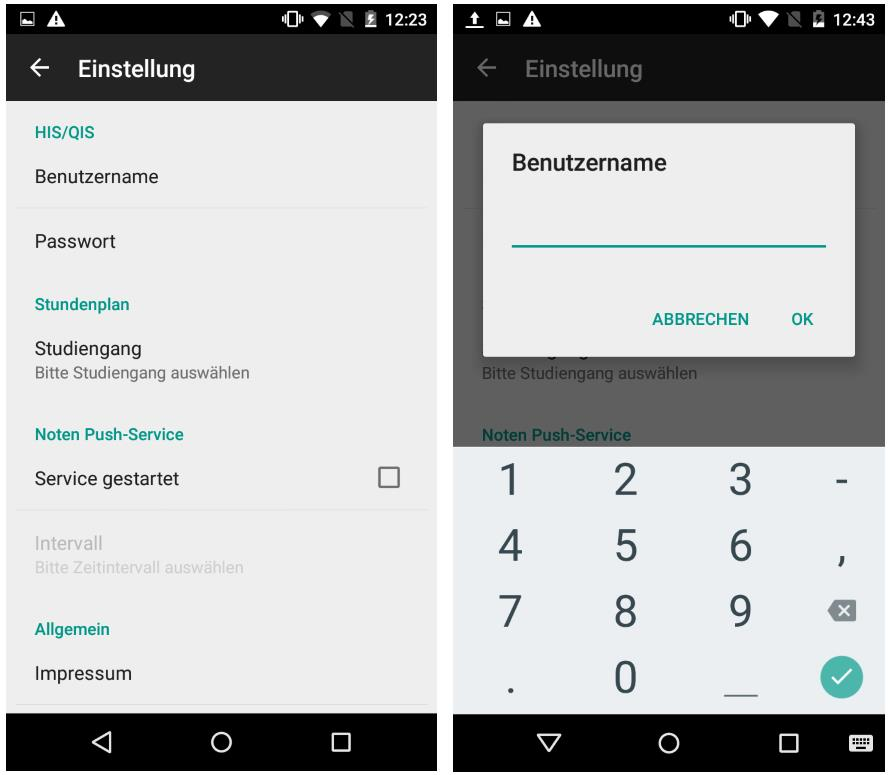
\includegraphics[scale=0.5]{03_Bedienungsanleitung/img/einstellungen.jpg}
        %\caption{Beispielbild b}
    \end{minipage}
    %\hfill
    \begin{minipage}{0.45\linewidth}
        \centering
        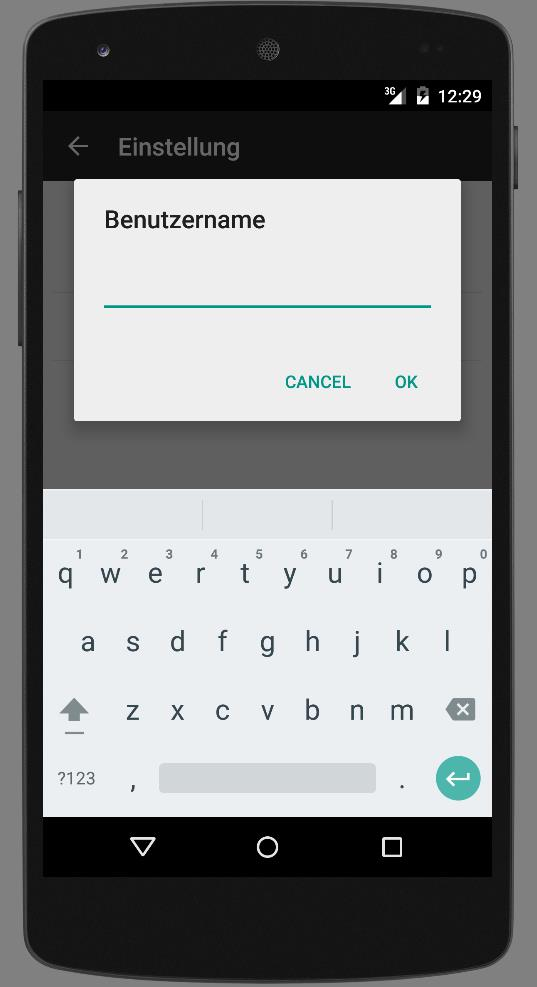
\includegraphics[scale=0.5]{03_Bedienungsanleitung/img/account.jpg}
        %\caption{Beispielbild b}
    \end{minipage}
\end{figure}

\newpage

Nach erfolgreichem Eintragen des Benutzeraccounts und verlassen der Einstellungen kann über den Menü-Button der Punkt "Noten" ausgewählt werden. Hier werden die aktuellen Noten aus QIS/HIS geladen und angezeigt. Sollte es beim Anmelden an QIS/HIS zu einem Fehler kommen, erscheint eine Fehlermeldung und die vorher vorgenommenen Einstellungen sollten noch einmal kontrolliert werden. 

\begin{figure}[h]
	\centering
	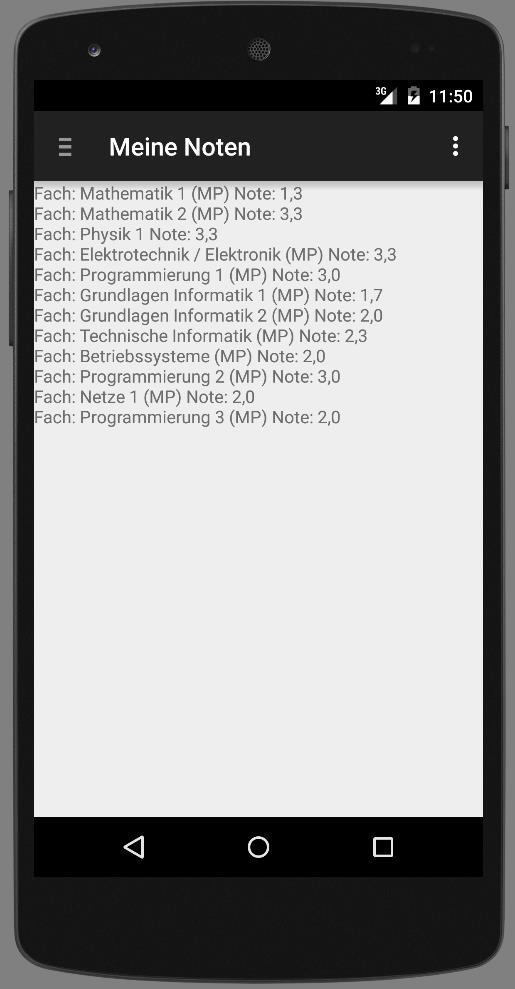
\includegraphics[scale=0.6]{03_Bedienungsanleitung/img/noten.jpg}
	%\caption{eine Grafik ohne Sinn und Verstand}
	\label{img:grafik-dummy}
\end{figure}

\newpage

\subsection{Stundenplan}

Den Stundenplan erreicht man über das Menü. Hat man in den Einstellungen vorher seinen Studiengang und das Matrikeljahr angegeben, erscheint der zu einem passende Stundenplan.

\begin{figure}[h]
	\centering
	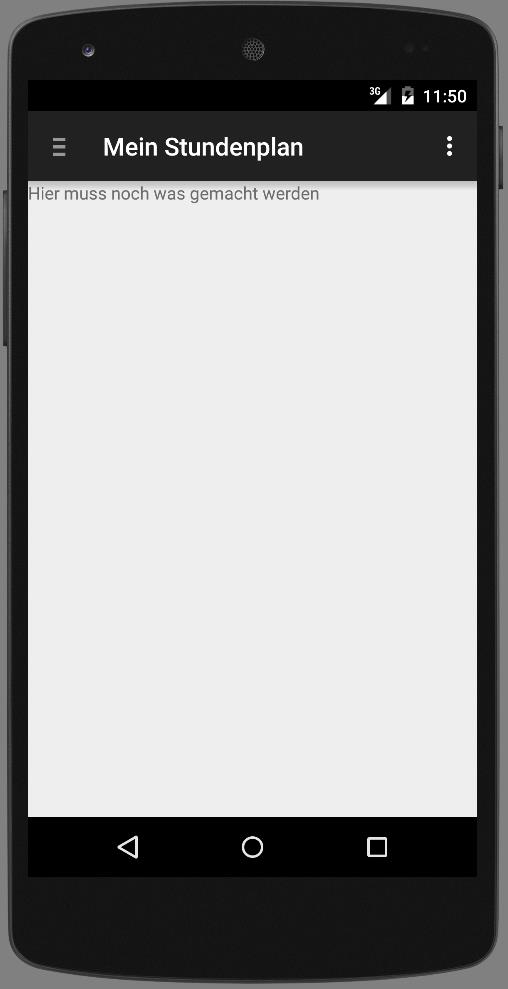
\includegraphics[scale=0.6]{03_Bedienungsanleitung/img/stundenplan.jpg}
	%\caption{eine Grafik ohne Sinn und Verstand}
	\label{img:grafik-dummy}
\end{figure}


\newpage

\newpage
\subsection{Entwicklerhandbuch}

\begin{figure}[h]
	\centering
	
\includegraphics[scale=0.5]{03_Bedienungsanleitung/img/Logo_HFTl_App.jpg}
	\label{img:grafik-dummy}
\end{figure}

\begin{center}
	{\huge Entwicklerhandbuch}
\end{center}

\begin{center}
	{\huge -  HfTL-APP  -}
\end{center}

\begin{center}
	\textbf{{\large Stand: {\today}}}
\end{center}

\newpage
\tableofcontents
\newpage

\subsubsection{Allgemeines}
Dieses Dokument dient lediglich als Hilfswerkzeug zur (Weiter-)Entwicklung und Wartung der HfTL-App. In diesem Dokument ist der grobe Aufbau, sowie die wichtigsten verwendeten Funktion mitsamt zugehörigen Quelltext erklärt.
\\[1em]
Dieses Dokument ist keine Programmieranleitung.
\\[1em]
Es empfiehlt sich, gewisse Grundkenntnisse in objektorientierter Programmierung im Allgemeinen und  in JAVA, XML und AndroidStudio im Speziellen mitzubringen, um dieses Dokument effizient nutzen zu können.
\\[1em]
Standard-Methoden und Klassen sind nicht im Detail erklärt, da das den Rahmen dieses Dokuments übersteigen würde. Für tiefer greifende Informationen wird die \href{http://developer.android.com/reference/packages.html}{Android-API} empfohlen.
\newpage
\subsubsection{Verwendete Software}
\paragraph{AndroidStudio}
\ \\[1em]
AndroidStudio ist die Standard-Entwicklungsumgebung für Android. Es bietet bereits ein fertiges Gerüst für eine funktionsfähige App an. Das Programm bietet Klassenbibliotheken, Debugger und selbst ein Emulator mit dessen Hilfe Android-Endgeräte auf dem PC virtuell dargestellt werden können.\\
Das Programm kann kostenlos unter \href{https://developer.android.com/sdk/index.html}{developer.android.com} heruntergeladen werden.



\paragraph{GitHub}
\ \\[1em]
GitHub ist ein onlinebasierter Dienst, der es einem ermöglicht, Dateien zu hosten und parallel im Team zu bearbeiten. Zudem bietet GitHub eine einfache und übersichtliche Form der Versionierung.\\
Durch des Erstellen unterschiedlicher Repositorys kann an mehreren Stellen eines Projekts gleichzeitig gearbeitet und getestet werden, ohne Datenverluste befürchten zu müssen.

\paragraph{Gimp}
\ \\[1em]
Gimp ist ein Open-Source Bildbearbeitungsprogramm. Es wurde in dem konkreten Fall genutzt, um Grafiken für die App zu erstellen.\\
Das Programm kann kostenlos auf der Seite des Herstellers  (\href{http://www.gimp.org/downloads/}{www.gimp.org}) herunter geladen werden.

\paragraph{Microsoft Office}
\ \\[1em]
MS Office ist das Office Paket von Microsoft, welches bei der Entwicklung der App nur eine beiläufige Rolle spiele. Genutzt wurde insbesondere MS Word zur schnellen Erstellung von Fließtext bzw. der Dokumentation. Die Eigentliche Aufbereitung des Textes erfolgte dann in LaTex.\\
Die Erstellung der Organigramme bzw. Pläne erfolgte durch MS Excel.

\paragraph{LateX}
\ \\[1em]
ist ein Softwarepaket, das die Benutzung des Textsatzsystems TeX mit Hilfe von Makros vereinfacht. 
Die Projektdokumentation wurde mit TeX entwickelt 

\newpage

\subsubsection{Aufbau des Projekts}
\subsubsubsection{Manifest.XML}
Diese Datei ist für jede Android-App zwingend notwendig. Hier werden grundsätzliche Dinge definiert, z.B. Welche Berechtigung diese App benötigt und auf welche Hardware im laufenden Zustand zugegriffen werden muss.
\\\
Des Weiteren wird hier auch das package für den Javaquellcode definiert:\\\
\lstset{language=XML}
\begin{lstlisting}[caption={AndroidManifest.XML},label=package, frame=single]
<manifest xmlns:android="..." package="bkmi.de.hftl_app" >
\end{lstlisting}
Die Zugriffsberechtigungen sind wie folgt definiert:\\\

\begin{lstlisting}[caption={AndroidManifest.XML},label=permissions, frame=single]
<uses-permission android:name="android.permission.INTERNET" />
<uses-permission android:name="android.permission.ACCESS_NETWORK_STATE" />
<uses-permission android:name="android.permission.READ_PHONE_STATE" />
\end{lstlisting}
Bei der Installation der App wird der Nutzer entsprechend informiert, dass die App auf die jeweiligen Funktionen des Endgerätes zugreift.
 \\\
In der manifest.xml ist ebenfalls eine Übersicht über die verwendeten Verzeichnisse und Komponenten hinterlegt, z.B. für die Activities.\\
Bei der HfTL-App ist der Verweis für die MainActivity (die Activity, mit der die App startet) für die NewsActivity gesetzt.
 \\\ 
Die folgenden Tags wurden bei der App nicht verwendet, sind aber theoretisch für Erweiterungen möglich:
\begin{lstlisting}[caption={Zugriffsbeispiel},label=perm-examble, frame=single]
<uses-feature android:name="android.hardware.camera" />
\end{lstlisting}
Das wäre ein Tag, um im laufenden Betrieb auf die Kamera des Telefons zuzugreifen.

\newpage

\subsubsubsection{Ordnerstruktur}
\begin{description}
\item[Database]~\par
\begin{itemize}
\item beinhaltet die NotenDB.java – Inhalt ist der Connector und die Kernfunktionen um Inhalte der eigentlichen Datenbank zu aktualisieren und zu modifizieren
\item NotenTabelle.java – das ist die eigentliche Datenbank, bzw. die eigentliche Definition vom Aufbau der Datenbank
\end{itemize}

 
\item[Fragmente]~\par
\begin{itemize}
\item beinhaltet die Fragmente, die von den Activties verwendet werden.
\end{itemize}

\item[Service]~\par
\begin{itemize}
\item beinhaltet die Datei NotenService.java, die zum Erzeugen von Push-Nachrichten dient, sobald es in der Notenübersicht neue Noten für den jeweiligen Studenten gibt.
\end{itemize}

 
\item[Help]~\par
\begin{itemize}
\item beinhaltet diverse Hilfsunktionen, die unter anderem zum Ausführen von Threads dienen.
\item[Ressourcen]~\par
\item unter /src/main/res befindet sich eine Ordnerstruktur, welche XML- und Bilddateien für verschiedenste Anwendungszwecke beinhaltet. Diese werden beim Kompilieren des Projekts in die Ressourcendatei R.java geschrieben. Über diese Datei, wird dann auf die Ressourcen zugegriffen. \\
Es wird im Weiteren nicht detailliert auf alle Dateien eingegangen. Es wird nur auf jene Dateien eingegangen, deren Inhalt zur Schilderung von wichtigen Kernfunktionen dienlich ist.
\end{itemize}

\newpage

\item[Activities]~\par
\begin{itemize}
\item Eine Activity stellt ein sichtbares Fenster dar, welches die eigentliche Interaktion mit dem Nutzer ermöglicht. Diese Interaktionen werden als Events bezeichnet bzw. behandelt. Durch sogenannte Intents ist es möglich andere Activitys zu starten. Der sichtbare Teil der Activity wird durch eine View definiert. Dort befinden sich dann die Eventauslöser, wie zum Beispiel \hyperref[button]{Buttons} etc. 
\item Folgende Grafik dient zur Übersicht:\\
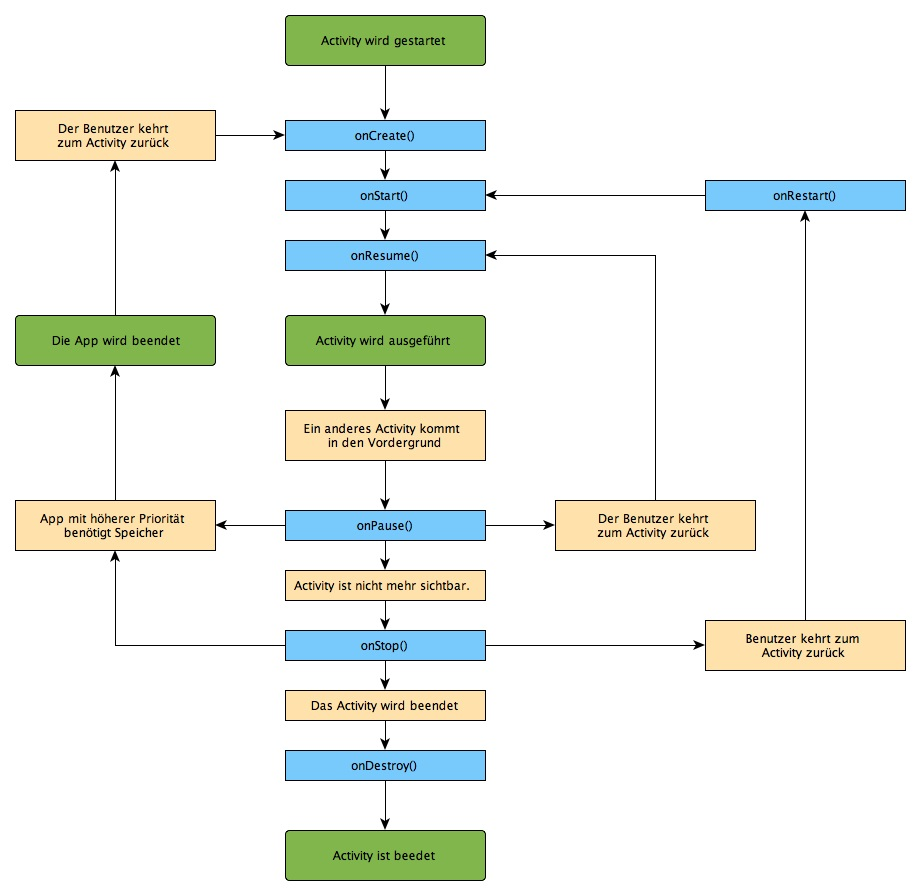
\includegraphics[scale=0.5]{05_Handbuch/img/AndroidActivityLebenszyklus.jpg}
\item Jede Activity hat einen sogenannten "'Lifecycle"' (=Lebenszyklus), der von dem Betriebssystem gesteuert und verwaltet wird. Dem Entwickler ist es nun überlassen, welche Ressourcen er entsprechend sichert, sollten die Ressourcen auf dem Mobiltelefon knapp werden. Das passiert in den Events:
\begin{itemize}
\item onPause$()$: die App ist noch sichtbar, aber nicht mehr im Vordergrund
\item onStop$()$: die App ist nicht mehr sichtbar
\end{itemize} 
\item Lifecycle einer Activity:\\
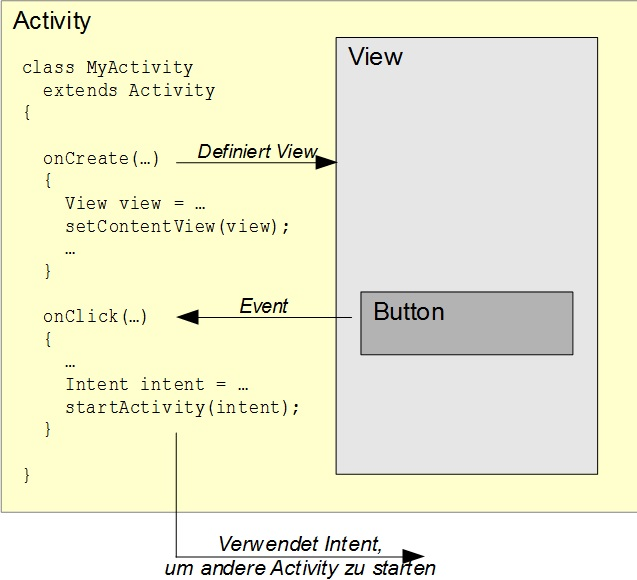
\includegraphics[scale=0.5]{05_Handbuch/img/Beginners_Workshop_Activity.jpg}
\end{itemize}

\newpage
 
\item[Fragmente]~\par
\begin{itemize}
\item In Android ist es nicht möglich, mehrere Activities gleichzeitig anzuzeigen, wenn es der Platz auf dem Display theoretisch erlauben würde. Um das dem Entwickler dennoch zu ermöglichen, bietet Android den Objekttypen "'Fragment"' an. 
\item Fragmente sind UI-Container, die über laufende Activities gelegt werden. Dies macht besonders dann Sinn, wenn es um die Fragmentierung der App geht (verschiedene Displaygrößen) bzw. wenn man zwischen den Ansichten wechselt (Haltung des Telefons)

\item Ebenso wie eine Activity hat ein Fragment ein Lifecycle, welcher in direkter Kommunikation mit dem Lifecycle der Activity steht. So werden zum Beispiel alle Fragmente eine Activity pausiert, wenn die Activity selbst pausiert wird. Folgendes Diagramm soll das veranschaulichen:\\
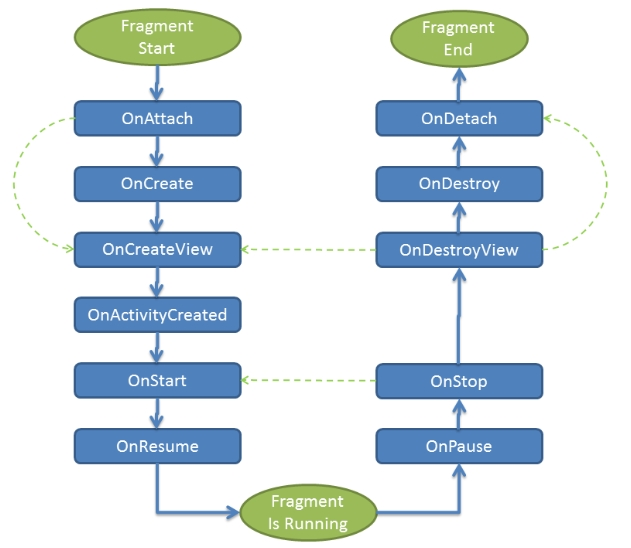
\includegraphics[scale=0.8]{05_Handbuch/img/LifeCycle_Fragment.jpg}
\end{itemize}

\newpage

\subsubsection{Activities}
\subsubsubsection{NewsActivity.java}\label{newsactitvity}
\begin{itemize}
\item Klasse wird mit Fragment extended
\item \hyperref[NavigationDrawerFragment]{NavigationDrawerFragment} wird benötigt, um die Interaktion mit Fragmenten der Anzeige zu ermöglichen
\item Intent wird benötigt, um andere Activities neben der NewsActivity zu handlen.
\item mTitle ist der Titel des zuletzt geladenen Screens
\end{itemize}

 
\item[onCreate()]~\par
\begin{itemize}
\item Hier wird das Layout geladen, welches in der zugehörigen xml definiert wurde
\item Laden des mNavigationDrawerFragment, zum Abbilden des Menüs am linken Seitenrand
\item Laden des Layouts für das Fragment
 
Durch das Laden des Layouts für das mNavigationDrawerFragment (durch setUp) wird die Funktion onNavigationDrawerItemSelected gerufen, weil in der Layoutdefintion Item 1 der Listview ausgewählt wird.
\end{itemize}
 
\item[onNavigationDrawerItemSelected()]~\par
\begin{itemize}
\item Durch das Aufrufen der Funktion wird das eigentliche Fragment für den FragmentManager ausgewählt (durch die switch-case-Anweisung) und abschließend durch das commit aktiv geladen.
\end{itemize}

 
\item[onSectionAttached()]~\par
\begin{itemize}
\item Je nach Auswahl wird hier mTitle aktualisiert.
\end{itemize}

 
\item[restoreActionBar()]~\par
\begin{itemize}
\item Dient zum Aktualisieren der Titelleiste (durch setTitle und mTitle als Argument)
\end{itemize}

 
\item[onCreateOptionsMenu()]~\par
\begin{itemize}
\item Erstellt das Menü oben rechts (drei Punkte) und befüllt es mit den Daten aus der /res/menu/news.xml
\end{itemize}

 
\item[onOptionsItemSelected()]~\par
\begin{itemize}
\item Überprüft welches Element aus dem Menü ausgewählt wurde
\end{itemize}

\newpage

\subsubsubsection{EinstellungsActivity.java}
 
\item[onCreate()]~\par
\begin{itemize}
\item Einbinden der "'einstellung.xml"' (beinhaltet Definitionen für Stringvariablen, Listen und Checkboxen)
\item Setzen von Startwerten für shared, check und list
\item Ausführen von registerPreferenceListener()
\end{itemize}

\item[registerPreferenceListener()]~\par
\begin{itemize}
\item Es wird ein anonymer Listener erstellt, der auf Änderungen in der SharedPreference.xml reagiert
\item In der Methode onSharedPreferenceChanged(SharedPreferences prefs, String key) werden die Änderungen abgefangen
\item Listener wird am SharedPreferences Objekt  registriert
\end{itemize}

\item[testeBenutzerdaten()]~\par
\begin{itemize}
\item Funktion zum Überprüfen von Anmeldedaten
\item via TextSecure ts wird Ver- und Entschlüsselung gewährleistet
\end{itemize}


 
\item[keineBenutzerdaten()]~\par
\begin{itemize}
\item Funktion zum Ausgeben, dass die Anmeldeinformationen falsch eingegeben wurden
\end{itemize}

\newpage

\subsubsection{NewsClickedActivity.java}
\label{NewsClickedActivity}
\lstset{language=JAVA}
\subsubsubsection{Allgemein}
Diese Activity wird geladen, sobald in der News-Übersicht (\hyperref[newsactitvity]{NewsActivity.java}) ein Eintrag geöffnet wird. \\
Der Inhalt wird durch NewsResolver und dessen Funktion getDetailsStringArray in das String-Array "'s"' geladen.
\item[onCreate()]~\par
\begin{itemize}
\item Laden des in der zugehörigen xml definierten Layouts (activity\_ news\_ clicked.xml)
\item Einbinden der "'Extras"' (Übergebene Variablen)
\item Zuweisung der URL aus dem rufenden NewsFragment
\item Aufruf des DetailHelpers durch 
\begin{lstlisting}
 new Detailhelper().execute();
\end{lstlisting}
\end{itemize}

\subsubsubsection{Klasse DetailHelper}
\item[onPreExecute()]~\par
\begin{itemize}
\item Anzeige eines ProgressDialogs (Ladebalken mit Hinweistext), um den Anwender zu informieren.
\begin{lstlisting}
ladebalken = ProgressDialog.show(NewsClickedActivity.this, "Bitte warten", "Nachricht wird geladen", true, false);
\end{lstlisting}
\end{itemize}

\item[onPostExecute()]~\par
\begin{itemize}
\item Ressourcen des ProgressDialogs werden freigegeben
\begin{lstlisting}
ladebalken.dismiss();
\end{lstlisting}
\item TextViews 1 bis 3 werden mit den Inhalten (Strings) befüllt.
\begin{lstlisting}
public void run() {
   tv1=(TextView)findViewById(R.id.tv_news_date);
   ...
   tv1.setText(s[%%2%%]);
}
\end{lstlisting}
\item Der User kann den Inhalt der TextViews kopieren und in die Zwischenablage des Endgeräts speichern.
\begin{lstlisting}
tv1.setTextIsSelectable(true);
\end{lstlisting}
\item Im TextView 4(\textit{Inhalt der News}) werden einige besondere Anweisungen benötigt:
\begin{itemize}
\item Darstellung und Verfolgung von (Hyper-)links.
\begin{lstlisting}
tv4.setClickable(true);
tv4.setMovementMethod(LinkMovementMethod.getInstance());
\end{lstlisting}
\item Verarbeitung des vom NewsResolver übergebenen HTML-Strings
\begin{lstlisting}
tv4.setText(Html.fromHtml(s[%%3%%]));
\end{lstlisting}
\end{itemize}
\end{itemize}

\item[doInBackground()]~\par
\begin{itemize}
\item Neuinstanzierung eines NewsResolvers mit übergebener Url, um durch die Funktion getDetailsStringArray das Array s mit Daten zufüllen
\begin{lstlisting}
 s[%%0%%]=elements.get(%%0%%).child(%%1%%).text()+"\n";   $$//Ueberschrift$$
 s[%%1%%]=elements.get(%%0%%).child(%%2%%).text()+"\n";   $$//Subhead$$
 s[%%2%%]=elements.get(%%0%%).child(%%0%%).text();        $$//Zeit$$
 s[%%3%%]=elements.get(%%0%%).child(%%0%%).outerHtml().replaceAll("<p>&nbsp;</p>", "");                   $$//Text$$
return s; 
\end{lstlisting}
\end{itemize}
\newpage
\subsubsection{Fragmente}
\subsubsubsection{NewsFragment}
Initialisierung erfolgt durch „NewInstance“, die aus der NewsActivity heraus gerufen wird. (siehe Funktionsaufruf -> onNavigationDrawerItemSelected)
Durch das .commit wird diese neue Instanz der Klasse dann geladen.
\paragraph{Überschriebene Funktionen}
\ \\[1em]
\item[OnAttach()]~\par
\begin{itemize}
\item Verknüpfung des NewsFragments mit der MainActivity
\end{itemize}

\item[OnCreateView()]~\par
\begin{itemize}
\item Hier wird lediglich das Layout der View des Fragments geladen und angewendet
\end{itemize}

\item[onActivityCreated()]~\par
\begin{itemize}
\item es wird geprüft, ob es SavedInstances (bereitsgeladene Inhalte) gibt
\item wenn JA:
\begin{itemize}
\item die Informationen werden aus dem ARRAYSPEICHER geholt und angewandt
\end{itemize}
\item wenn NEIN:
\begin{itemize}
\item die Funktion „zeigeNews“ wird gerufen, welche die aktuellsten News vom Server lädt
\end{itemize}
\end{itemize}

 
\item[onStart()]~\par
\begin{itemize}
\item in dieser Funktion wird nur noch der Listener für den Aktualisierbutton mit der Schaltfläche verknüpft. Als onClick-Event wird dann lediglich die Funktion „zeigeNews“ gerufen.
\end{itemize}

\newpage
 
\paragraph{standAllone-Funktionen}
\  \\[1em]
\item[isOnline()]~\par
\begin{itemize}
\item Diese Methode prüft durch einen Connectivity Manager, ob eine Verbindung zum Internet besteht
\end{itemize}

\item[zeigeNews()]\label{zeigenews}~\par
\begin{itemize}
\item Zunächst wird durch „isOnline“ geprüft, ob eine aktive Netzverbindung besteht
\item wenn NEIN:
\begin{itemize}
\item Es wird ein Hinweis an den Nutzer ausgegeben
\end{itemize}
\item wenn JA: 
\begin{itemize}
\item Es wird eine Instanz der Klasse \hyperref[NewsHelper]{NewsHelper} erstellt, welche dann als Hintergrund-Task ausgeführt wird, um ein Einfrieren der App zu verhindern.
\end{itemize}
\end{itemize}
\newpage
\subsubsubsection{Klasse NewsHelper}
\label{NewsHelper}
\begin{itemize}
\item Klasse mit asynchroner Task-Ausführung
\item Nach dem Aufruf der Methode \textit{zeigenews} wird durch den Unterfunktionsaufruf \textit{.execute} zunächst die Funktion \textit{doInBackground} ausgeführt, wo eine neue Instanz des NewsResolvers erstellt wird.
\begin{lstlisting} 
private void zeigeNews(){
 NewsHelper nh = new NewsHelper();
 nh.execute();
}
\end{lstlisting}   
\item Durch \textit{getTermineStringArray} des NewsResolvers wird ein String-Array zurückgegeben.
\item Danach wird die Methode \textit{onPostExecute} gerufen.
\end{itemize}
\item[onListItemClick()]~\par
\begin{itemize}
\item Es wird ein intent verwendet um die \textit{NewsClickedActivity} zu starten, als "'Übergabeparameter"' wird \textit{putExtra} verwendet, im Falle der App die URL zu dem angeklickten Event.
\begin{lstlisting}
 intent = new Intent(getActivity(), NewsClickedActivity.class);
 intent.puExtra(TERMINDETAIL, newsResolver.getURLAsString(position));
 startActivity(intent);
\end{lstlisting}
\end{itemize}

\item[onPostExecute()]~\par
\begin{itemize}
\item  Überprüfung ob das Fragment noch aktiv ist
\begin{lstlisting}
if(getActivity()==null) return;
\end{lstlisting}
\item einbinden des \hyperref[CustomAdapterNews]{CustomAdapterNews} in die ListView
\begin{lstlisting}
setListAdapter(new CustomAdapterNews(getActivity(), ...);
\end{lstlisting}
\end{itemize}
\newpage
\subsubsubsection{NavigationDrawerFragment}\label{NavigationDrawerFragment}
\begin{itemize}
\item Dieses Fragment bildet das Menü auf dem linken Rand der App ab und aktiviert den Button mit dem man in die Einstellungen gelangt.
\end{itemize}

\item[onCreate()]~\par
\begin{itemize}
\item In dieser Methode werden die Einstellungen der Activity übernommen und der Drawer ausgewählt. 
\item Außerdem wird geprüft ob eine gesicherte Instanz vorhanden ist, aus der dann das zuletzt ausgewählte Fragment ermittelt wird und über die Funktion \textit{selectItem()} aufgerufen wird. 
\item Falls keine gespeicherte Instanz existiert, wird die "'0"' (\textit{NewsFragment}) als Standardwert übergeben.
\end{itemize}
 
\item[onActivityCreated()]~\par
\begin{itemize}
\item Hier wird das Menü für das aktuelle Fragment aktiviert indem an \textit{setHasOptionsMenu()} "'\textcolor{darkblue}{true}"' übergeben wird.
\end{itemize} 
\item[onCreateView()]~\par
\begin{itemize}
\item In dieser Funktion wird das Design für die Actionbar (als Listview) und die dazugehörigen Menüpunkte festgelegt. 
\item Zudem wird hier der ClickListener initialisiert, der dann den ausgewählten Eintrag an \textit{selectItem()} übergibt.
\end{itemize}

\item[isDrawerOpen()]~\par
\begin{itemize}
\item Diese Methode prüft ob der Drawer bereits offen ist und liefert einen Wahrheitswert zurück.
\end{itemize} 
\item[setUp()]~\par
\begin{itemize}
\item Es werden hier folgende Einstellungen vorgenommen:
\begin{itemize}
\item Einstellungen zum Design
\item Aktivierung des HomeButtons und dessen Animation beim Draufklicken
\item Zusammenführung der \textit{ActionBar} und des \textit{NavigationDrawers}
\item weitere Einstellungen zum Drawer
\end{itemize}
\item Dann wird die Konfiguration in \textit{mDrawerToggle} abgespeichert
\end{itemize}

\item[selectItem()]~\par
\begin{itemize}
\item Hier wird die Animation auf den angeklickten Menüpunkt ausgeführt.
\item Zudem wird der Drawer geschlossen und die Position des angeklickten Punktes an \textit{mCallbacks.onNavigationDrawerItemSelected()}  übergeben.
\end{itemize} 
\item[onAttach()]~\par
\begin{itemize}
\item Diese Methode setzt den Zeiger mCallbacks auf die Activity.
\end{itemize}
 
\item[onDetach()]~\par
\begin{itemize}
\item Hier wird der Zeiger \textit{mCallbacks} auf "'\textcolor{darkblue}{null}"' gesetzt.
\end{itemize}
\item[onSaveInstanceState()]~\par
\begin{itemize}
\item Diese Funktion sichert die aktuelle Instanz.
\end{itemize}
\item[onConfigurationChanged()]~\par
\begin{itemize}
\item Bei einer Änderung in den Einstellungen konfiguriert diese Methode \textit{mDrawerToggle} um.
\end{itemize} 
\item[onCreateOptionsMenu()]~\par
\begin{itemize}
\item Diese Funktion legt das Design, aus einer XML-Datei für das Menü Einstellungen, fest.
\end{itemize} 
\item[onOptionsItemSelected()]~\par
\begin{itemize}
\item Hier wird der Button, über den man zu den Einstellungen gelangt, aktiviert und mit dessen Klasse verknüpft.
\end{itemize}
\item[NavigationDrawerCallbacks()]~\par
\begin{itemize}
\item Hier wird die ausgewählte Menüpunkt-ID an die Activity übergeben.
\end{itemize}
\newpage
\subsubsubsection{Notenfragment}
\item[onCreateView()]~\par
\begin{itemize}
\item Laden des entsprechenden XML-Layouts \textit{fragment\_ noten.xml}
\item Laden und Zuweisung der Schriftart des TextViews für die Überschrift des Fragments
\end{itemize}

\item[onAttach()]~\par
\begin{itemize}
\item Aufruf der Datenbank, in der die Noteneinträge abgelegt werden
\end{itemize}

 
\item[onDetach()]~\par
\begin{itemize}
\item Schließen der Datenbank
\end{itemize}

 
\item[onStart()]~\par
\begin{itemize}
\item Erstellen des Buttons zum Aktualisieren
\item Mittels \textit{OnClickListener} für den Button, wird über die Methode \textit{testeBenutzerdaten()} überprüft, ob die Benutzerdaten für QiS eingetragen wurden. Andernfalls erfolgt die Ausgabe mittels der Methode \textit{keineBenutzerdaten()}, dass diese nicht eingetragen wurden. 
\item Sofern die Benutzerdaten eingetragen wurden, und eine Onlineverbindung zu QiS besteht, werden die Noten erneut abgerufen. 
\item Ist keine Verbindung zu QiS vorhanden, wird der Nutzer mittels Toast-Benachrichtigung darüber informiert
\item[] 
\includegraphics[scale=0.5]{05_Handbuch/img/Noten_Toast.jpg}
\end{itemize}
\item[getNoten()]~\par
\begin{itemize}
\item Liest in der Notendatenbank alle Werte in der Spalte \textcolor{lila}{NOTENABFRAGE} aus und schreibt diese in das String-Array "'\textit{s}"', welches auch übergeben wird.
\end{itemize}

 
\item[getSemester()]~\par
\begin{itemize}
\item Liest in der Notendatenbank alle Werte in der Spalte \textcolor{lila}{SEMESTERABFRAGE} aus und schreibt diese in ein String-Array "'\textit{s}"', welches auch übergeben wird. 
\end{itemize} 
\item[getFach()]~\par
\begin{itemize}
\item Liest in der Notendatenbank alle Werte in der Spalte \textcolor{lila}{FACHABFRAGE} aus und schreibt diese in das String-Array "'\textit{s}"', welches auch übergeben wird.
\end{itemize}

\item[getVersuche()]~\par
\begin{itemize}
\item Liest in der Notendatenbank alle Werte in der Spalte \textcolor{lila}{VERSUCHABFRAGE} aus und schreibt diese in das String-Array "'\textit{s}"', welches auch übergeben wird.
\end{itemize}
\item[Hinweis:]~\par \textit{Die String-Arrays sind nur lokal in den jeweiligen Methoden definiert, weshalb diese - der Einfachheit halber - alle den Namen "'\textit{s}"' erhielten. Tatsächlich werden hier vier unterschiedliche String-Arrays befüllt.}
 
\item[setzeListview()]~\par
\begin{itemize}
\item Hier werden zunächst entsprechende String-Arrays durch die jeweiligen Methoden zur Abfrage in der Datenbank befüllt:
\begin{lstlisting}
notenList = getNoten();
semesterList = getSemester();
fachList = getFach();
versuchList = getVersuche();
\end{lstlisting}
\begin{itemize}
\item Die Strings stehen entsprechend der alphabetischen Reihenfolge der Semesterbeschreibung in den Arrays.
\item Bsp: SoSe 12, SoSe 13, WiSe 11/12, WiSe 12/13, WiSe 13/14
\end{itemize}

\item Um die Übersichtlichkeit zu wahren, werden die Werte in den Arrays nun sortiert, wobei die Werte vom aktuellsten Semester am Anfang stehen und anschließend chronologisch geordnet werden.
\item Um dies zu realisieren wird zunächst mit Hilfe eines regulären Ausdrucks ein Suchpattern festgelegt, nach dem die zu sortierenden Elemente gefunden werden.
\item Entscheidend für die Sortierung sind die letzten beiden Ziffern für die Jahreszahl.
\begin{lstlisting}
Pattern p = Pattern.compile("\\d{2}$");
\end{lstlisting}
\item Anschließend wird der Einfachheit halber ein Bubblesort  verwendet (kann ggf. geändert werden), der durch das String-Array \textcolor{lila}{semesterList} geht und bei benachbarten Einträgen den Suchpattern anwendet.
\begin{lstlisting}
Matcher m = p.matcher(semesterList[j]);
Matcher n = p.matcher(semesterList[j+1]);
\end{lstlisting}

\item Sofern die Pattern in den beiden Einträgen vorhanden sind (das ist eine zwingende Bedingung), werden diese jeweils in Hilfsvariablen geschrieben.
\begin{lstlisting}
if((m.find())&&(n.find())){
 int x = Integer.parseInt(m.group());
 int y = Integer.parseInt(n.group());
 ...}
\end{lstlisting}
\item Danach werden diese Hilfsvaribalen verglichen und ggf sortiert. 
\item Sofern die Einträge in (\textcolor{lila}{semesterList}) sortiert werden, müssen auch die zugehörigen Werte in den anderen Arrays (\textcolor{lila}{notenList}, \textcolor{lila}{fachList}, (\textcolor{lila}{versuchList}) entsprechend sortiert werden.
\begin{lstlisting}
if(x<y){
  temps = semesterList[j];
  semesterList[j] = semesterList[j+1];
  semesterList[j+1] = temps;
  temps = notenList[j];
  notenList[j] = notenList[j+1];
  notenList[j+1] = temps;
  temps = fachList[j];
  ...
  }
\end{lstlisting}

\item Sobald die Sortierung erfolgt ist, müssen noch redundante Werte im Array (\textcolor{lila}{semesterList}) gefunden und durch (\textcolor{darkblue}{NULL}) ersetzt werden.
\begin{itemize}
\item Dadurch wird eine Auflistung der Noten, Fächer und Versuche, aufgeschlüsselt nach Semester realisiert, ohne dass über jedem Eintrag die Semesterbeschreibung steht. ( s. \hyperref[CustomAdapterNoten]{CustomAdapterNoten.java})
\begin{lstlisting}
String[] vgl = new String[1];
vgl[0]="";
for(int k=0; k<semesterList.length;k++){
   if (semesterList[k].equals(vgl[0])) {
      vgl[0] = semesterList[k];
      semesterList[k] = null;
   }
   else{
      vgl[0] = semesterList[k];
   }
}
\end{lstlisting}
\end{itemize}

\item Anschließend werden diese String-Arrays an den \hyperref[CustomAdapterNoten]{CustomAdapterNoten} übergeben. Damit wird eine individuelle Befüllung und Formatierung der Liste mit den ausgelesenen Werten aus der Datenbank realisiert.
\end{itemize} 
\item[keineBenutzerdaten()]~\par
\begin{itemize}
\item Diese Methode prüft, ob in den Einstellungen Login und Passwort für QiS eingetragen wurden. Andernfalls wird eine Fehlermeldung ausgegeben:
\item[] 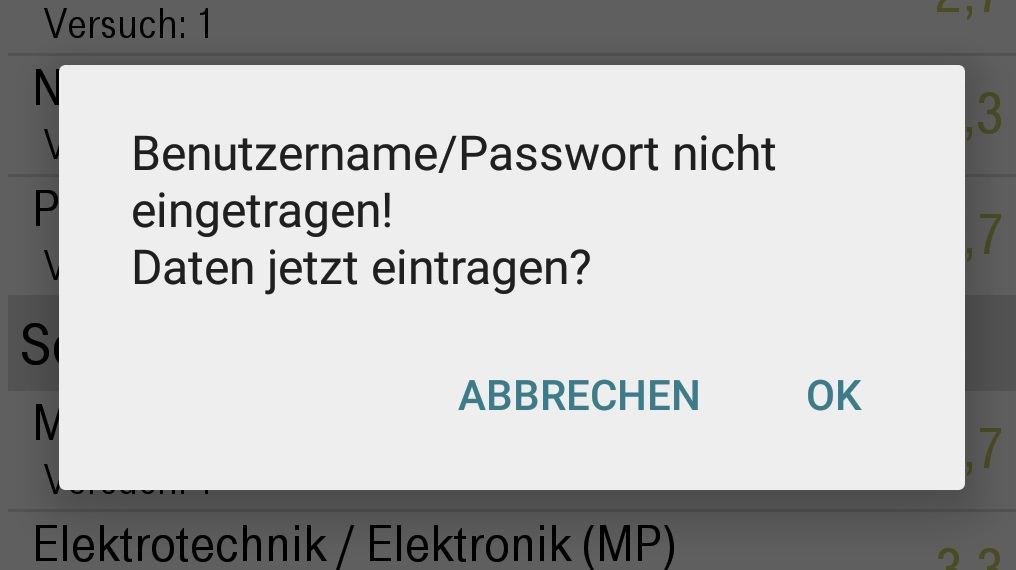
\includegraphics[scale=0.5]{05_Handbuch/img/Benutzerdaten.jpg}
\end{itemize}
 
-- NotenHelper (Class)

\newpage

\subsubsubsection{StundenplanFragment}

\item[newInstance()]~\par
\begin{itemize}
\item Erstellt ein StundenplanFragment und "'steckt"' die aktive Position (aus dem Navigation Drawer) in das "'Bundle args"' welches als Argument im Fragment übergeben wird.
\end{itemize} 
\item[onCreateView()]~\par
\begin{itemize}
\item Laden des entsprechenden XML-Layouts fragment\_ noten.xml
\item Laden und Zuweisung der Schriftart für das TextView für die Überschrift des Fragments.
\end{itemize}

\item[onViewCreated()]~\par
\begin{itemize}
\item Falls im "'\textit{Stundenplanspeicher}"' Daten vorhanden sind, werden diese geladen.
\item Methode für das Dropdownmenü wird gerufen und Array für "'events"' erstellt.
\item Anonyme Listener für die Buttons werden erstellt.
\end{itemize}

\item[erzeugeDropdown()]~\par
\begin{itemize}
\item Dropdown aus xml einem Objekt zuweisen.
\item Listener für Dropdown (als anonymer Listener) wird erzeugt und registiert.
\item Beim registieren wird die Methode \textit{onItemSelected} aufgerufen und ein StundenplanHelper ausgeführt.
\item Mittels eines "'\textit{Calendar}"', "'\textit{Date}"' und zwei "'\textit{SimpleDateFormat}"' wird das Dropdownmenü befüllt, indem die Daten in eine String-List eingefügt werden (\textit{list.add(temp)}).
\item Dropdown wird mit Liste verknüpft.
\end{itemize}
 
\item[keinStudiengang()]~\par
\begin{itemize}
\item Prüft ob in den Einstellungen der Studiengang eingetragen wurde, ansonsten wird eine Fehlermeldung ausgegeben:
\item[] 
\includegraphics[scale=0.5]{05_Handbuch/img/Studiengang.jpg}
\end{itemize}

\item[erstelleStundenplan()]~\par
\begin{itemize}
\item Erzeugt die Ausgabe des Stundenplans und fügt sie in den ListView ein.
\item Falls keine Daten vorhanden sind, wird "'keine Daten"' ausgegeben.
\end{itemize}
 
-- StundenplanHelper (class)
 
\item[onPreExecute()]~\par
\begin{itemize}
\item erzeugt einen Ladebalken.
\end{itemize}
\item[onPostExecute]~\par
\begin{itemize}
\item falls das Fragment noch aktiv ist wird die Methode erstelleStundenplan() gerufen.
\item Ladebalken wird entfernt.
\end{itemize}
 
\item[doInBackground]~\par
\begin{itemize}
\item Die Methode erzeugt einen \textit{StundenplanResolver} und
befüllt das “StundenplanEvents-Array \textit{Events}“ mit Daten durch die Methode \textit{erzeugeStundenplan(String woche)} des StundenplanResolvers.
\item Falls ein Fehler auftritt, wird ein Event erstellt, in dem keine Daten sind.
\end{itemize}

\newpage
\subsubsection{CustomAdapter} 
\subsubsubsection{Allgemein} 
Die CustomAdapter kommen da zum Einsatz, wo eine ListView genutzt und individuell befüllt werden muss. \\
\begin{itemize}
\item[1]Fragment.java wird mittels inflate der fragment.xml zugeordnet
\item[2]Fragment.java übergibt die zuvor ermittelten Daten  (mit Strings befüllte Arrays) an den CustomAdapter
\item[3]Entsprechend der Länge x der Arrays wird x-mal die zugehörige \_list.xml als LayoutContainer aufgerufen und ihre TextViews mit den Inhalten der Arrays befüllt.
\item[4]Die befüllten LayoutContainer werden zeilenweise an die ListView in der fragment.xml übergeben.
\end{itemize}
\item[] 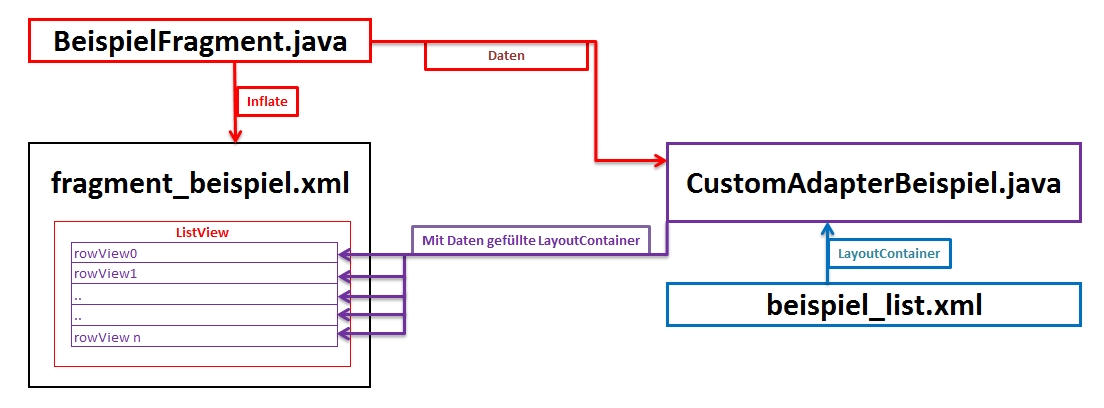
\includegraphics[scale=0.5]{05_Handbuch/img/CustomAdapter.jpg} \\

\newpage

\item [class Holder]~\par
Dies ist ein Container mit TextViews
\begin{lstlisting}
   TextView tv_name;
\end{lstlisting}
Dieser Container wird dann als jeweilige Zeile in der ListView der zugehörigen Activity dargestellt.\\
Die Grundlage der Ausgabe bilden spezielle XML-Dateien. Diese dienen definieren die Output jeder einzelnen Zeile der ListViews. Hier sind Name, Position, Dimensionen, Farben, \hyperref[Schriftarten]{Schriftarten}, Schriftgröße etc festlegt.\\ 
Für jeden Customadapter gibt es eine entsprechende \_list.xml:
\begin{itemize}
\item news\_list.xml
\item noten\_list.xml
\item stundenplan\_list.xml
\end{itemize}

\item [public View getView()]~\par
erstellt einen neuen Container: 
\begin{lstlisting}
   Holder holder = new Holder;
\end{lstlisting}
erstellt eine View rowView:
\begin{lstlisting}
   View rowView;
\end{lstlisting}
Das Layout der View und damit jeder Zeile in der ListView wird durch das Laden der entsprechenden XML namelist formatiert:
\begin{lstlisting}
   rowView = inflater.inflate(R.layout.name_list, null);
\end{lstlisting}
Die TextViews des Containers werden den entsprechenden TextViews in der XML zugeordnet:
\begin{lstlisting}
   holder.tv_name=(TextView)
   rowView.findViewbyId(R.id.namelist_name.xml);
\end{lstlisting}
Das TextView wird mit dem entsprechenden Wert des zugehörigen String-Arrays befüllt:
\begin{lstlisting}
   holder.tv_name.setText(name[position]);
\end{lstlisting}
Der nun befüllte Container wird nun als rowView übergeben:
\begin{lstlisting}
   return rowView;
\end{lstlisting}
\newpage

\subsubsubsection{CustomAdapterNews.java}
\label{CustomAdapterNews}
Dies ist der simpelste CustomAdapter der HfTL-App. Er wird verwendet um die News-Liste (also die Übersicht der News aus der HfTL-Homepage) zu formatieren.\\
Dabei werden drei String-Arrays (date, headline, content) in das zugehörige TextView der rowView übergeben. Der Inhalt dieser Arrays wird mittels der Klasse \hyperref[Newshelper]{NewsHelper}, die wiederum die Methoden der Klasse NewsResolver aufruft, befüllt.
\subsubsubsection{CustomAdapterNoten.java}
\label{CustomAdapterNoten}
Dieser CustomAdapter wird für die Befüllung der ListView des Notenfragments benutzt.\\
Hier werden vier String-Arrays (\textcolor{lila}{subject}, \textcolor{lila}{trys}, \textcolor{lila}{mark}, \textcolor{lila}{semester}) mit den Daten aus der Notendatenbank befüllt.\\
Entsprechend des Inhalts, werden die zugehörigen TextViews noch gesondert formatiert.\\
Ist der Inhalt an der Position des String-Arrays "'\textcolor{darkblue}{NULL}"', wird das zugehörige TextView auf "'\textcolor{lila}{GONE}"' gesetzt. So wird realisiert, dass mehrere Fächer unter dem selben Semester gelistet sind, ohne dass ein leeres (dunkelgraues) TextView erscheint.
\begin{lstlisting}
   if(semester[position]==null){
    holder.tv_semester.setVisibility(TextView.GONE);
   }
\end{lstlisting}
Auch für die jeweiligen Noten gibt es eine gesonderte Formatierung:
\begin{itemize}
\item Note schlechter als 5.0: \textcolor{magentat}{magenta}
\item Note schlechter als 3,4: \textcolor{gelbt}{gelb}
\item Note besser als 3,5: \textcolor{gruent}{gr"un}
\end{itemize}
\begin{lstlisting}
   if (mark[position].equals("5,0" ))
    holder.tv_mark.setTextColor
     (context.getResources().getColor(R.color.magenta));
   else if (mark[position].equals("4,0" ) |
            mark[position].equals("3,9" ) |
            mark[position].equals("3,8" ) |
            mark[position].equals("3,7" ) |
            mark[position].equals("3,6" ) |
            mark[position].equals("3,5" ) )
              holder.tv_mark.setTextColor
               (context.getResources().getColor(R.color.gelb));
       else
            holder.tv_mark.setTextColor
             (context.getResources().getColor(R.color.gruen));
\end{lstlisting}
\newpage
\subsubsubsection{CustomAdapterStundenplan}
\label{CustomAdapterStundenplan}
Dieser CustomAdapter befüllt die ListView des StundenPlanfragments.\\
Hier werden fünf StringArrays(\textcolor{lila}{datum},\textcolor{lila}{fach},\textcolor{lila}{zeit},\textcolor{lila}{raum},\textcolor{lila}{kategorie}) übergeben, die zuvor mittels der Methode \textit{erstelleStundenplan()} des StundenplanFragments aus dem HTML-Code der QiS/HiS-Seite ausgelesen wurden.\\
Auch hier gibt es einige spezifische Formatierungen, abhängig vom übergebenen Inhalt.\\
Ist der Inhalt des StringArrays \textcolor{lila}{datum} an einer Stelle "'\textcolor{darkblue}{NULL}"', so wird die Sichtbarkeit des zugehörigen TextViews auf  "'\textcolor{lila}{GONE}"' gesetzt.\\
Analog zum \hyperref[CustomAdapterNoten]{CustomAdapterNoten} werden so die einzelnen Fächer unter dem selben Datum gelistet. Andernfalls würde über jedem Fach ein dunkelgraues TextView stehen.
\begin{lstlisting}
if(datum[position]!=null)
   holder.tv_date.setText(datum[position]);
else
   holder.tv_date.setVisibility(TextView.GONE);
\end{lstlisting}
Das StringArray \textcolor{lila}{kategorie} wird - neben der reinen Ausgabe - dazu verwendet, wichtige Ereignisse farblich kenntlich zu machen. Dabei wird der Inhalt an der jeweiligen Position des StringArrays geprüft und eine entsprechende (CI/CD-)Farbe für das Rechteck auf der rechten Seite gesetzt:

\begin{itemize}
\item Prüfung: \textcolor{magentat}{magenta}
\item Praktikum: \textcolor{dunkelblaut}{dunkelblau}
\item Rest: \textcolor{grau01t}{grau01}
\end{itemize}
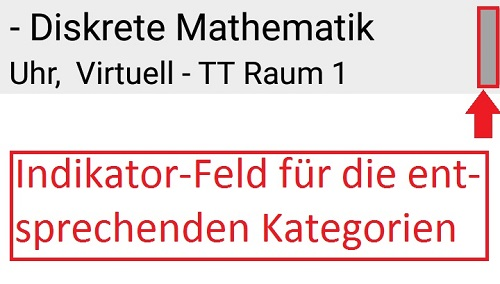
\includegraphics[scale=0.5]{05_Handbuch/img/kategorie.jpg}
\begin{lstlisting}
if (kategorie[position].equals("Pruefung"))
   holder.tv_category.setBackgroundColor
   (context.getRessources().getColor(R.color.magenta));
else if ((kategorie[position].equals("Praktikum"))
   holder.tv_category.setBackgroundColor
   (context.getRessources().getColor(R.color.dunkelblau));
else
    holder.tv_category.setBackgroundColor
   (context.getRessources().getColor(R.color.grau01));

\end{lstlisting}
\newpage
\subsubsection{XML-Dateien}
\label{XML}
\subsubsubsection{fragment.xml}
Die fragment.xml bilden das visuelle Rückgrat der App. Hier wird das Layout festgelegt und damit wo welcher Inhalt steht bzw. zu stehen hat. Statische Inhalte und Formatierungen(Farben, Dimensionen, Elementposition, Schriftarten etc.) werden bereits hier festgelegt.\\
Variable Formatierungen und Inhalte werden entweder direkt durch die zugehörige \textit{Fragment.java} oder - wenn sie die ListViews betreffen - durch den zugehörigen \hyperref[CustomAdapter]{CustomAdapter} befüllt.\\
Auf den detaillierten Aufbau wird nicht näher eingegangen, da dieser mit einigen XML-Kenntnissen selbsterklärend sein dürfte.

\subsubsubsection{\_list.xml}
Hier gibt es derzeit drei XML-Dateien:
\begin{itemize}
\item news\_list.xml
\item noten\_list.xml
\item stundenplan\_list.xml
\end{itemize}

Diese dienen als LayoutContainer für die ListViews. Sie werden durch den entsprechenden \hyperref[CustomAdapter]{CustomAdapter} mit den Daten aus der Fragment.java befüllt und zeilenweise an das zugehörige ListView der Fragment.xml übergeben.

\subsubsubsection{activity\_news\_clicked.xml}
Dient als Designvorlage für eine aufgerufene News aus der Newsübersicht. Der Inhalt wird durch die Klasse \hyperref[NewsClickedActivity]{NewsClickedActivity.java} befüllt.

\subsubsubsection{settings\_toolbar}
Definiert die Kopfzeile der einstellung.xml.

\subsubsubsection{impressum.xml \& activity\_impressum}
Hier steht das Impressum. Während das Layout in der activity\_impresum.xml festgelegt wird, wird der Inhalt (\textit{\"Ahnlich wie bei strings.xml})zentral abgelegt.

\subsubsubsection{colors.xml}
Um den Aufruf der Farben nach CI/CD zu vereinfachen, wurden die RGB-Werte (in hexadezimal) zentral in der Datei main\textbackslash res \textbackslash values \textbackslash colors.xml gespeichert.
\lstset{language=XML}
\begin{lstlisting}
<item name="magenta" type="color">#E20074</item>
<item name="grau01" type="color">#A4A4A4</item>
...
 <integer-array name="telekomcolors">
   <item>@color/magenta</item>
   <item>@color/grau01</item>
   ...
 </integer-array>
\end{lstlisting}
Die Farben können dann sowohl mittels JAVA als auch mittels XML aufgerufen werden:
\begin{itemize}
\item XML:
\begin{lstlisting}
android:color="@color/magenta"
\end{lstlisting}
\item JAVA:
\lstset{language=JAVA}
\begin{lstlisting}
getResources().getColor(R.color.magenta)
\end{lstlisting}
\end{itemize}



\subsubsubsection{array.xml}
Hier stehen alle aktuellen Studiengänge mit Matrikel und ihre zugehörigen Links zu QiS.\\
Ein Studiengang muss in den Einstellungen ausgewählt werden, damit der Stundenplan angezeigt werden kann.\\
Ferner sind hier die Werte für das Intervall der Notenabfrage abgelegt.\\
Die Pflege der Datei erfolgt derzeit manuell. (s. \hyperref[pflege]{Pflege der array.xml})

\subsubsubsection{einstellung.xml}
Layout-Definition des Einstellungsmenüs.

\subsubsubsection{strings.xml}
Statische Strings, wie sie beispielsweise für die Fragmentüberschriften verwendet werden, werden nicht in den XML-Tag geschrieben. 
\lstset{language=XML}
\begin{lstlisting}
<TextView
...
android:text="News aus der HFT-Leipzig"
.../>
\end{lstlisting}

Vielmehr werden diese zentral in der \textit{strings.xml} abgelegt.

\begin{lstlisting}[caption={Ablage in strings.xml}]
<string name="News_headline">News aus der HFT-Leipzig</string>
\end{lstlisting}

Anschließend werden diese Strings dort abgerufen, wo sie benötigt werden. 

\begin{lstlisting}[caption={Aufruf im fragment.xml}]
<TextView
...
android:text="@string/News_headline"
.../>
\end{lstlisting}



\newpage
\subsubsection{Layout}
\subsubsubsection{Allgemeines}
Das Layout wird zum Großteil über die \hyperref[XML]{XML-Dateien} realisiert. Um die Handhabung zu realisieren, wurden einige Elemente bzw. Bezeichnungen standardisiert.\\ Im Folgenden werden die wichtigsten Details rund um die Darstellung des Layouts erläutert. Mit einigen XML-Kenntnissen sollte der Großteil selbsterklärend sein.
\subsubsubsection{Schriftarten}
\label{Schriftarten}
Da die Standardbibliothek von Android nur sehr wenige Schriftarten liefert, mussten die Schriftarten nach CI/CD nachträglich eingefügt werden. Diese befinden sich unter main\textbackslash{assets}\textbackslash{fonts}.
Der Aufruf der Schriftarten erfolgt im Allgemeinen über folgende JAVA-Anweisung:
\lstset{language=JAVA}
\begin{lstlisting}[caption={Beispiel: Einbinden der Schriftart Ocra im Notenfragment}]
View notenView = inflater.inflate(R.layout.fragment_noten, container, false);

TextView hl = (TextView) notenView.findViewById(R.id.hl_Noten);
Typeface headline = Typeface.createFromAsset(getActivity().getAssets(), "fonts/OCRA.TTF");
hl.setTypeface(headline);

return notenView;
\end{lstlisting}
In der Praxis hat sich jedoch herausgestellt, dass diese Art und Weise, Schriftarten einzubinden auf zwei Probleme trifft:
\begin{itemize}
\item Über das Fragment können die Schriftarten nicht den ListViews zugewiesen werden, da bei Erstellung der Fragmente die ListViews bzw. deren Inhalt (die durch die jeweiligen CustomAdapter befüllt werden) noch nicht existieren.
\item Es wäre möglich die Schriftarten im jeweiligen CustomAdapter zuzuweisen. Jedoch hat die Praxis gezeigt, dass dadurch der Speicherverbrauch extrem ansteigt (200 bis 300 Prozent) und damit die Performance der App merkbar sinkt. Der Grund hierfür liegt daran, dass bei jedem TextView, das angezeigt wird, die Schriftarten aus den Assets geladen und im Cache abgelegt werden.
\end{itemize}
Das Problem wurde durch einige Anpassungen umgangen:
\begin{itemize}
\item Erstellen der Klasse FontCache
\begin{itemize}
\item Diese Klasse prüft ob die geforderten Schriftarten bereits im Cache hinterlegt sind.
\item Sollten die Schriftarten bereits im Cache hinterlegt sein, dann werden diese genommen. Andernfalls werden sie aus den Assets geladen und im Cache abgelegt.
\end{itemize}
\item Einbinden der Schriftarten in jeweilige Klassen
\begin{itemize}
\item Die Klassen werden direkt durch die TextViews in den XML-Dateien aufgerufen.
\item Beim Aufruf wird die o.g. Klasse \textit{FontCache} aufgerufen.
\end{itemize}
\item Setzen der Schriftarten in den XML-Dateien
\begin{itemize}
\item Um die benötigten Schriftarten zu laden, werden die XML-Tags geändert.
\begin{itemize}
\item Ursprüngliche (native) XML-Tags:
\lstset{language=XML}
\begin{lstlisting}[caption={Normales TextView}]
<TextView
  android:id="@+id/newslist_date"
  android:layout_width="wrap_content"
  android:layout_height="wrap_content"
  ... />
\end{lstlisting}
\item Pfadangabe zur jeweiligen Schriftart als neues XML-Tag:
\begin{lstlisting}[caption={Einbinden von  TeleGrotNorm}]
<bkmi.de.hftl_app.help.Typefaces.TeleGrotNorm
  android:id="@+id/newslist_date"
  android:layout_width="wrap_content"
  android:layout_height="wrap_content"
  ... />
\end{lstlisting}
\end{itemize}
\end{itemize}
\end{itemize}




\newpage
\subsubsubsection{Buttons}
\label{button}
Grundlegend werden vier Standardbuttons in der App verwendet. Sie alle wurden über eine eigene XML-Datei definiert und durch die XML-Dateien der jeweiligen Fragmente aufgerufen. Die Methoden, die bei Betätigung der Buttons aufgerufen werden, befinden sich in der JAVA-Datei des jeweiligen Fragments.\\
Durch die Auslagerung der Definitionen für die Buttons ist es u.a. möglich, Farbverläufe, abgerundete Ecken und interaktives Verhalten (bspw. Farbänderungen bei Betätigung) festzulegen. Im Grunde genommen wird nur ein \textit{Item} generiert, das als Vorlage für einen Button herhalten muss.\\


\item[Exemplarischer Button]~\par
\begin{itemize}
\item Es gibt drei Zustände:
\begin{itemize}
\item gedrückt
\begin{lstlisting}
<item android:state_pressed="true"> ... </item>
\end{lstlisting}
\item fokussiert
\begin{lstlisting}
<item android:state_focused="true"> ... </item>
\end{lstlisting}
\item standard
\begin{lstlisting}
<item> ... </item>
\end{lstlisting}
\end{itemize}
\item Der Status \textit{focused} wird derzeit nur als Dummy angesehen, da er derzeit nicht Verwendung ist.
\item Die Definitionen innerhalb der Items findet jeweils zwischen diesen Tags statt:
\begin{lstlisting}
<item>
   <shape> ... </shape>
</item>
\end{lstlisting}
\begin{itemize}
\item Farbverlauf mit Start- und Endfarbe, sowie dem Winkel des Farbverlaufs.
\begin{lstlisting}
<gradient
  android:startColor="#77E20074" 
  android:endColor="#E20074"     
  android:angle="270"/>           
\end{lstlisting}
\item Umrandung
\begin{lstlisting}
<stroke
   android:width="3dp"
   android:color="@color/hellblau"/>
\end{lstlisting}
\item Rundung der Ecken
\begin{lstlisting}
<corners
   android:radius="5dp"/>
\end{lstlisting}
\end{itemize}
\end{itemize}

Folgende Standardbuttons werden benutzt:

\item[custom\_button]~\par
\begin{itemize}
\item Dies ist der Standard-Button.
\end{itemize}
\item[custom\_newsclick]~\par
\begin{itemize}
\item Hier werden die News-Einträge der News-Übersicht als Button verwendet, um ein optisches Feedback zu erhalten, wenn eine News ausgewählt wurde.
\end{itemize}
\item[custom\_vorbutton \& custom\_zurbutton]~\par
\begin{itemize}
\item Diese beiden Buttons werden beim Stundenplan verwendet. (Grüne Dreiecke um zwischen den Wochen vor- und zurückzublättern.)
\item[] 
\includegraphics[scale=0.5]{05_Handbuch/img/Stundenplan.jpg}
\item als Vorlage dienen jpg-Images
\item Je nach Status werden die entsprechenden Images geladen:
\begin{itemize}
\item inaktiv:  \textcolor{grau01t}{grau}
\item aktiv: \textcolor{gruent}{gr\"un}
\item gedrückt (optisches Feedback): \textcolor{magentat}{magenta}
\end{itemize}
\end{itemize}
\newpage
\subsubsection{Erweiterungen und Verbesserungen für kommende Versionen}
Da es aufgrund der Projektrahmenbedingungen nicht möglich gewesen ist, alle gewünschten Features zu implementieren, folgt hier eine Auflistung weiterer Funktionen oder Verbesserungen, die für die App denkbar wären.
\subsubsubsection{Pflege der array.xml}\label{pflege}
Die Datei array.xml dient als Grundlage für das Einstellungsmenü.\\
Hier werden alle Studiengänge, mit den entsprechenden Matrikeln aufgelistet. Das Kernproblem ist, dass diese Liste manuell auf dem aktuellen Stand gehalten werden muss.\\
Denkbar wäre hier eine Methode, die zu gewissen Zeitpunkten (\textit{Ende der Semesterferien}) die neuen Matrikel hinzufügt. Problematisch dabei sind jedoch mehrere Aspekte, die beachtet werden müssen:
\begin{itemize}
\item Festlegung der Zeitpunkte zur Aktualisierung der Daten
\item Wegfall der alten Matrikel (Vermeidung von Datenmüll)
\item Umbenennung von Studiengängen
\item Hinzufügen neuer Studiengänge
\item Wegfall alter Studiengänge
\end{itemize}
Die Problemstellung ist damit für das Projekt zu komplex und kann wahrscheinlich besser in Absprache und Zusammenarbeit mit dem Hochschul- und Prüfungsamt der HfTL  gelöst werden.
\subsubsubsection{Raumplan}
Ein Kernfeature, das aber von der Komplexität her wohl ein eigenes Projektteam beschäftigen kann, ist die Raumplanung.\\
Hierbei soll es dem Nutzer bspw. möglich sein, freie Räume für selbst organisiertes Lernen zu finden.\\ Wichtig dabei ist auch zu wissen, wann welcher Raum durch wen belegt ist. Insofern müsste es abseits von der zentralen Raumplanung durch die HfTL möglich sein, dass der Nutzer sich einen freien Raum buchen kann und dieser Buchungswunsch dann auch für andere Anwesende zu sehen ist.\\
Idealerweise gäbe es auch einen Lageplan, wo welcher Raum zu finden ist.
\subsubsubsection{Portierung auf andere Systeme}
Die hier beschriebene App ist eine reine Android-App. Sofern es eine Nachfrage gibt, wäre eine Portierung auf andere Betriebssysteme (iOS, Windows Mobile, Ubuntu Touch und weitere) sicherlich sinnvoll.

\subsubsubsection{Bekannte Fehler}
Es gibt einige Bugs bzw. Fehler die in zukünftigen Versionen behoben werden müssen:
\begin{itemize}
\item Ist kein Email-Cient auf dem Smartphone installiert, kann womöglich die App abstürzen, wenn in den News ein Mail-Link aufgerufen wird.
\item Sind in den News auf der Homepage der HfTL Links nicht absolut angegeben (\textit{bspw. \textless a href ="'de/aktuelles/news.html"'\textgreater}), dann stürzt die App ab. 
\end{itemize}
\end{description} 


\subsection{Gantt}
\begin{landscape}
	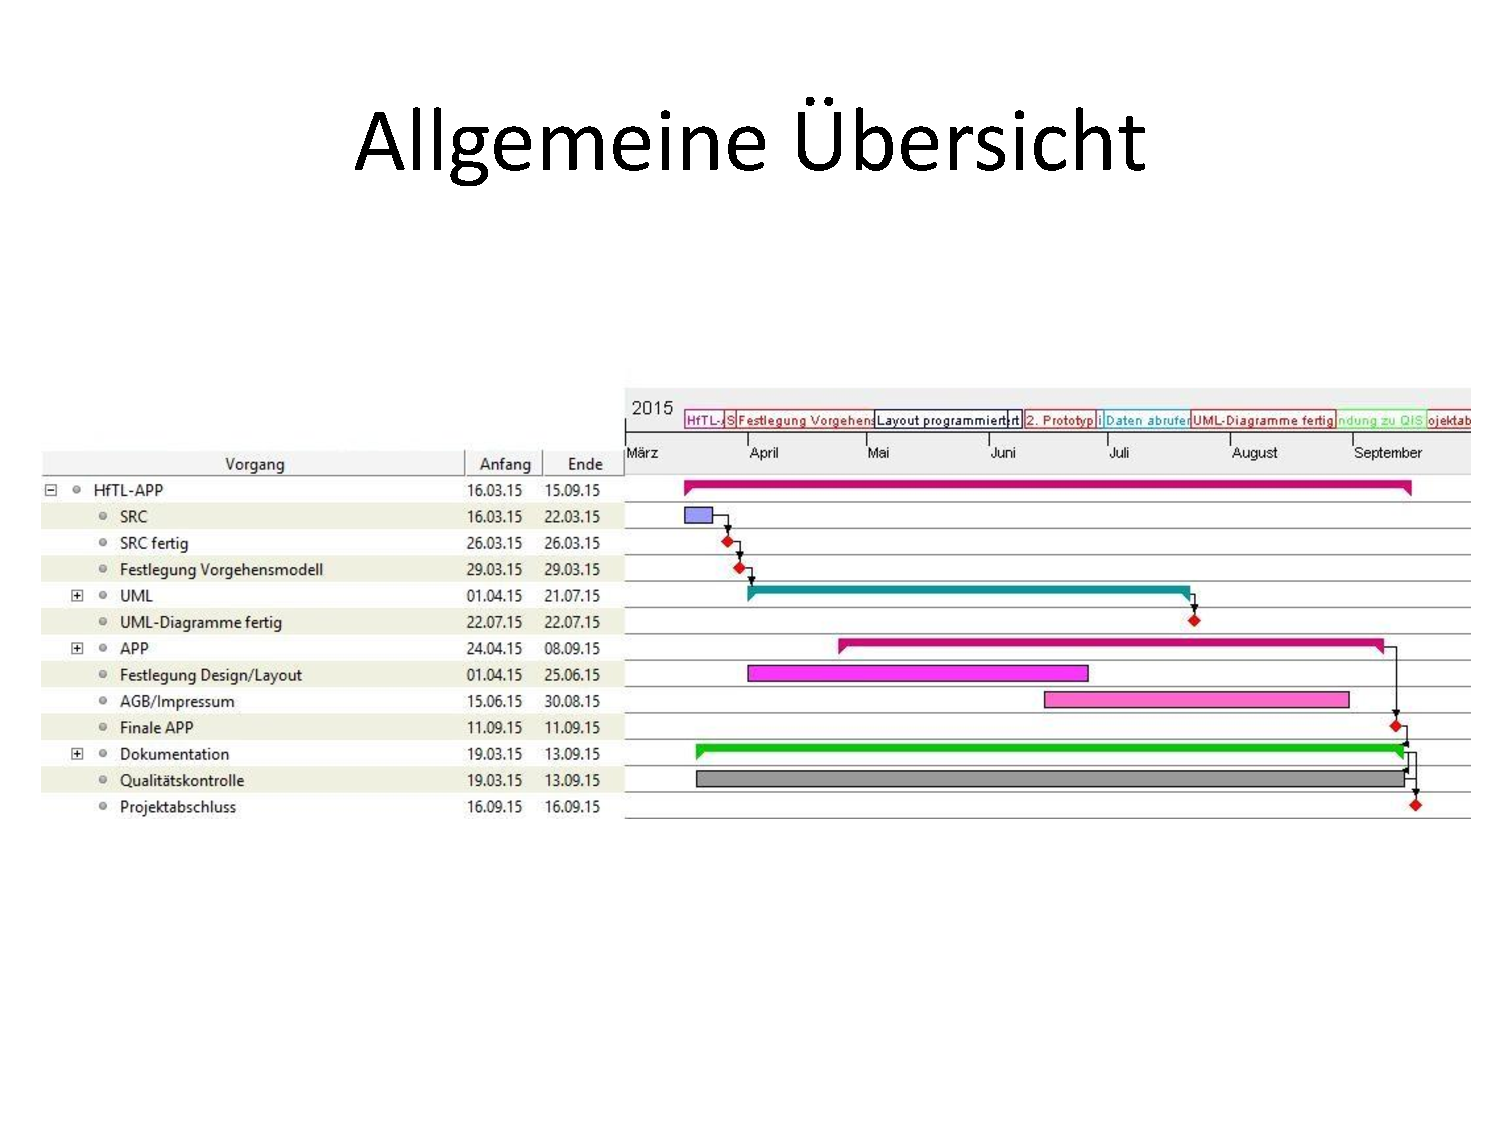
\includepdf[landscape=true,pages=-,noautoscale]{04_Anhang/files/Gant_HfTL-APP_Stand_30062015.pdf}
\end{landscape}

\subsection{App-Layout}
\label{subsec:App-Layout}
	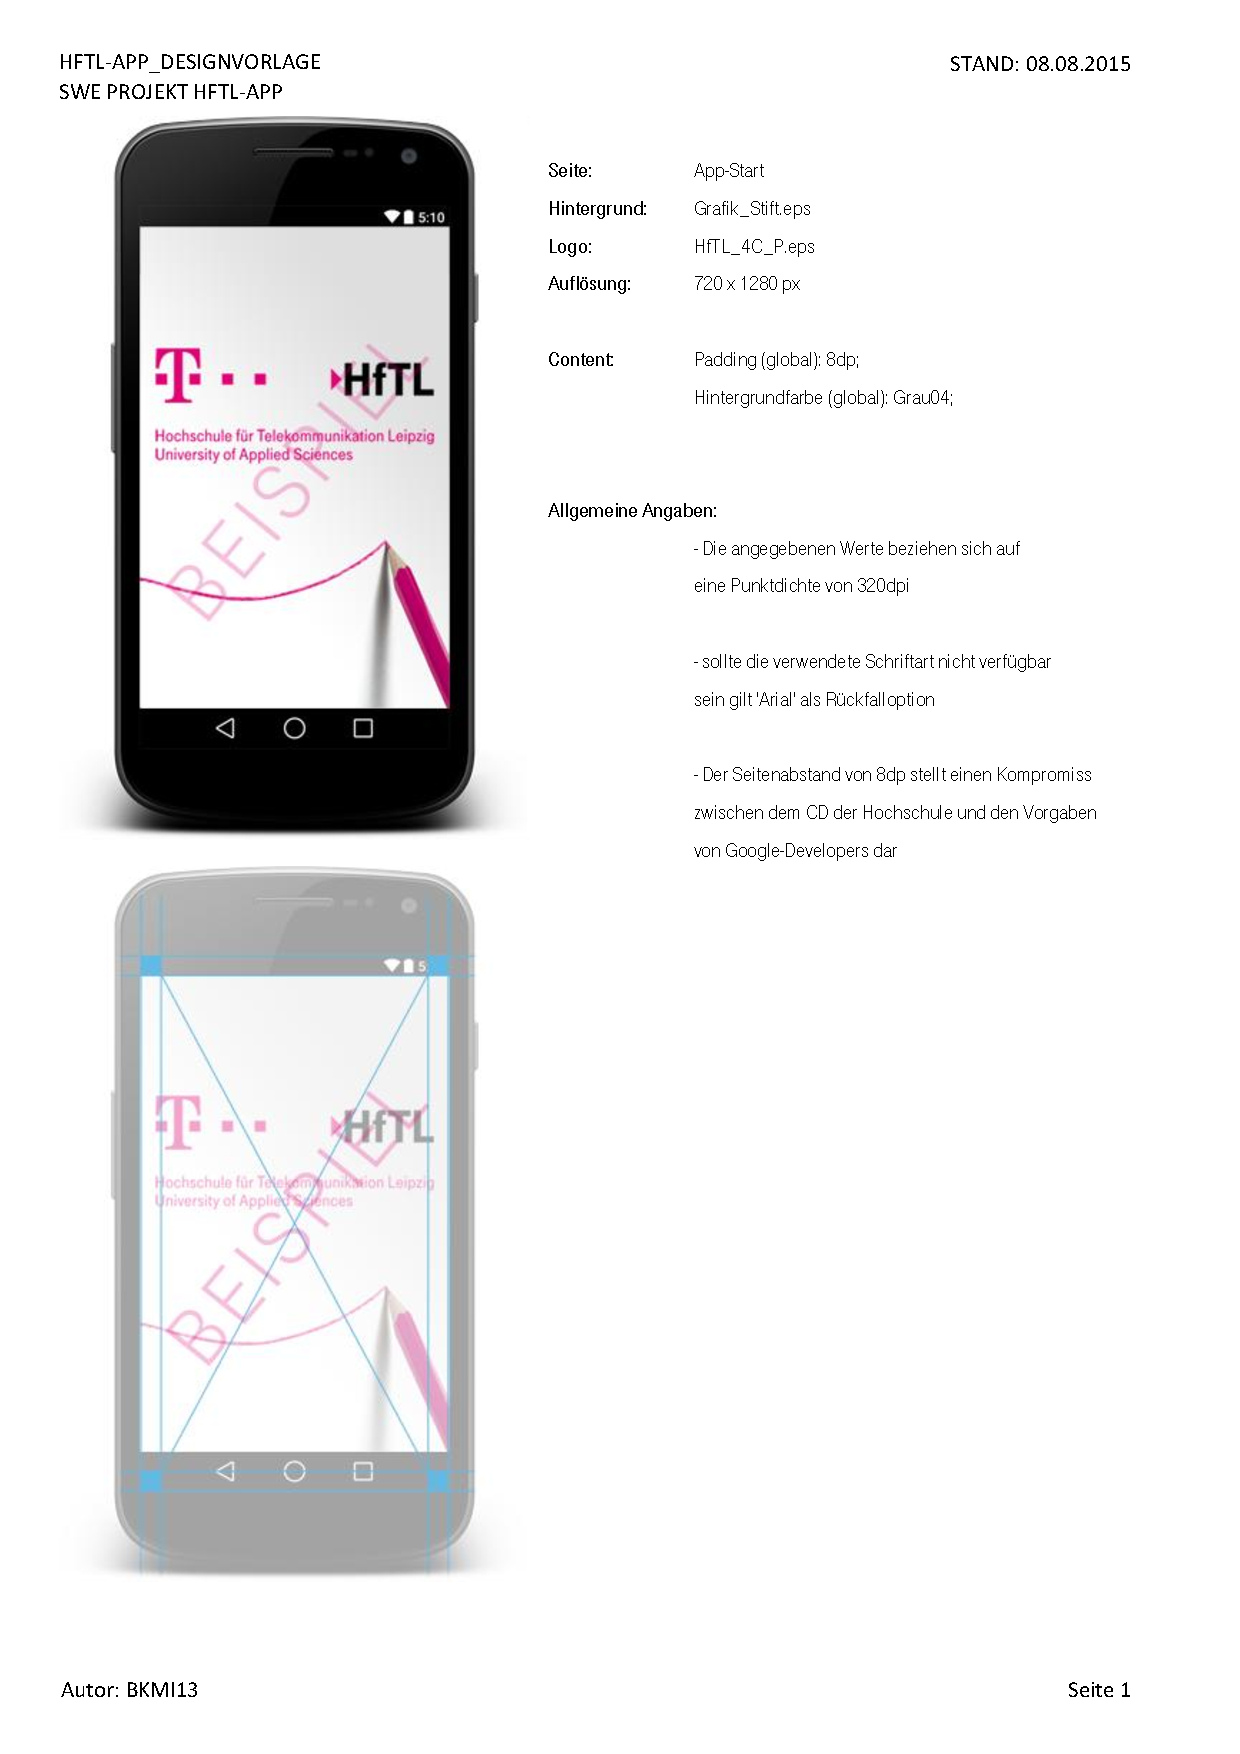
\includepdf[pages=-,noautoscale]{04_Anhang/files/HFTL-App_Designvorlage.pdf}
	
\subsection{Release-Historie}
\label{subsec:Release-Historie}
	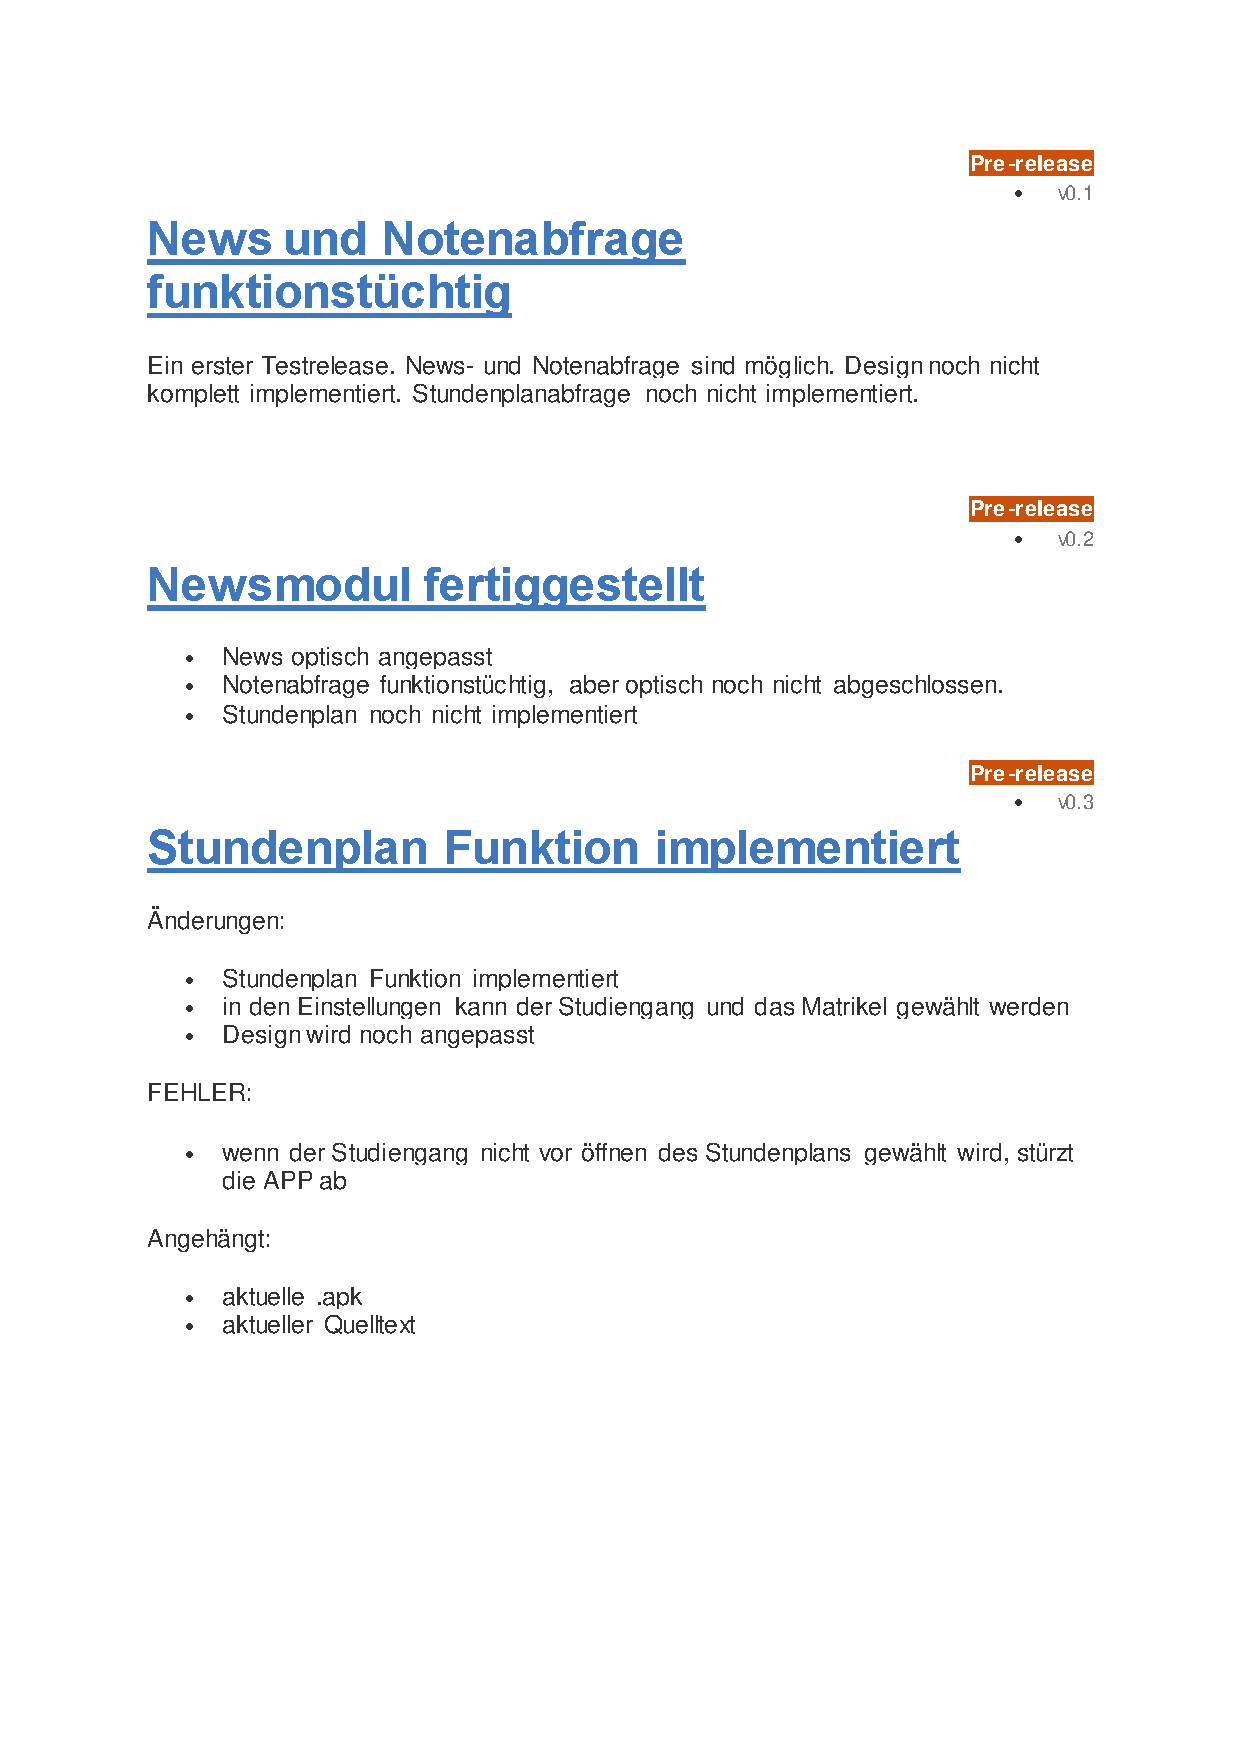
\includepdf[pages=-,noautoscale]{04_Anhang/files/Release_History.pdf}	
	
\subsection{Testprotokollentwurf}
\label{subsec:Testprotokollentwurf}
	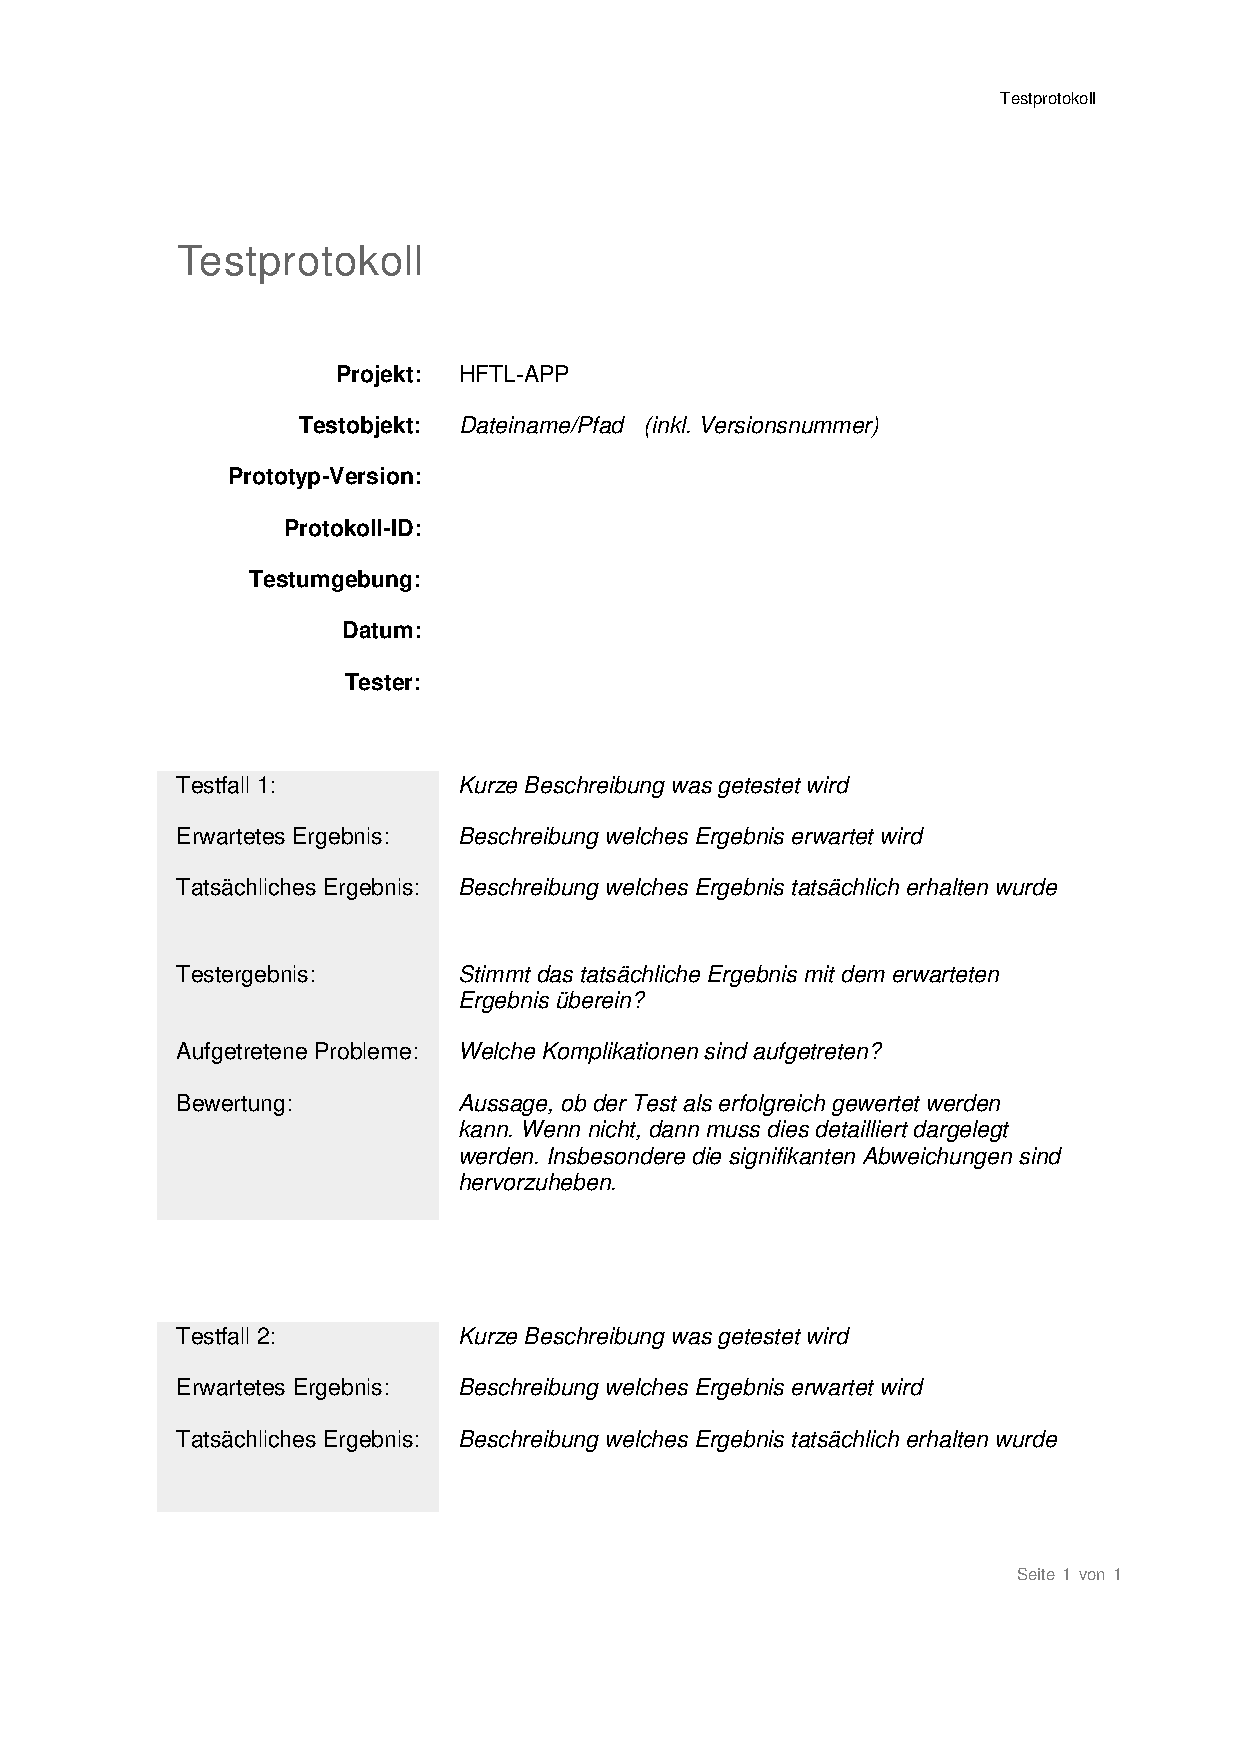
\includepdf[pages=-,noautoscale]{04_Anhang/files/Vorlage_Testprotokoll.pdf}
	
	

%%%%%%%%%%%%%%%%%%% Testprotokolle %%%%%%%%%%%%%%%%%%%%%%%%%%%%%%

	
\subsection{Testprotokolle}
\label{subsec:Testprotokolle}

\Large{Gesamtprotokolle}

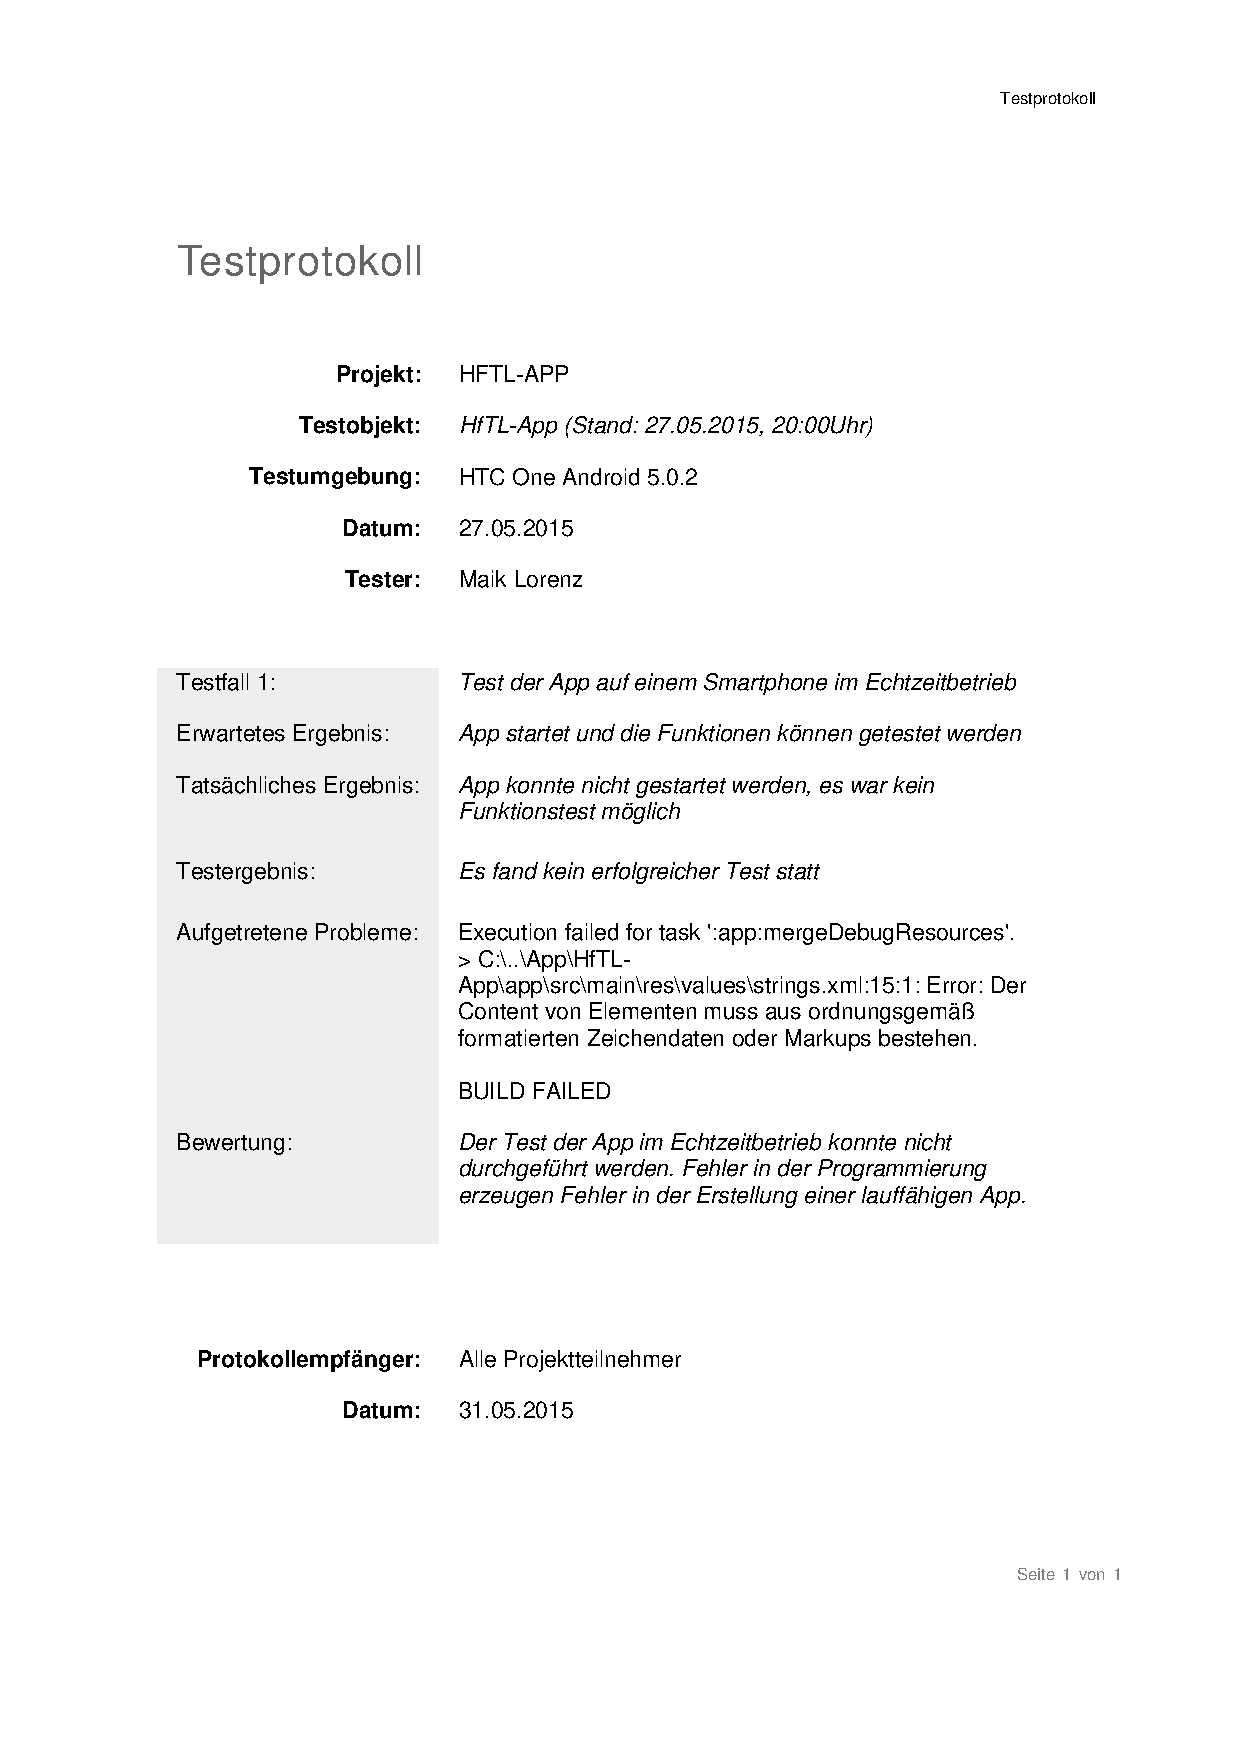
\includepdf[pages=-,noautoscale]{04_Anhang/files/Testprotokolle/Gesamt/150527_Testprotokoll_ML.pdf}
	
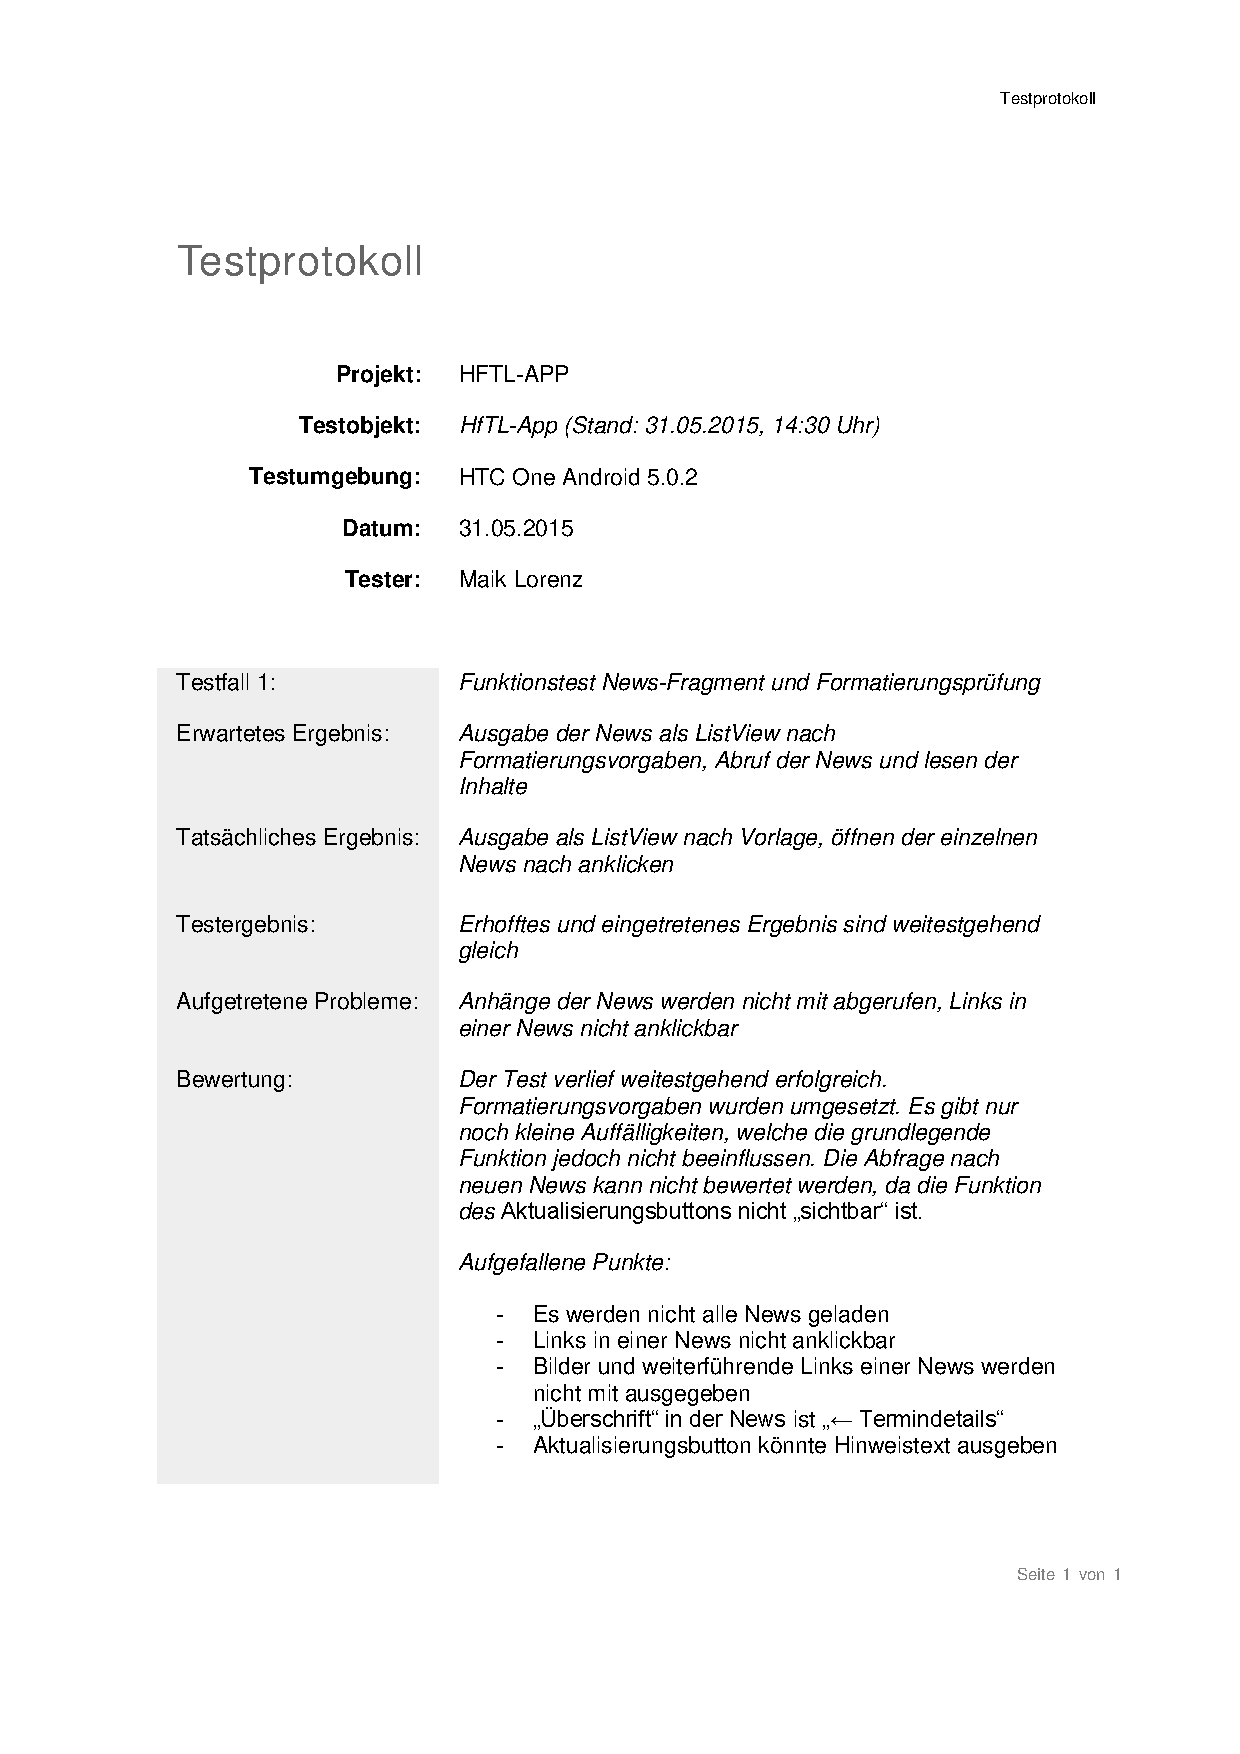
\includepdf[pages=-,noautoscale]{04_Anhang/files/Testprotokolle/Gesamt/150531_Testprotokoll_ML.pdf}
	
	
%%%%%%%%%%%%%%%%%%%%%%%%%%%%%%%%%%%%%%%%%%%%%%%%%%%%%%%%%%%%%%	
\Large{Testprotokolle zum News Modul}

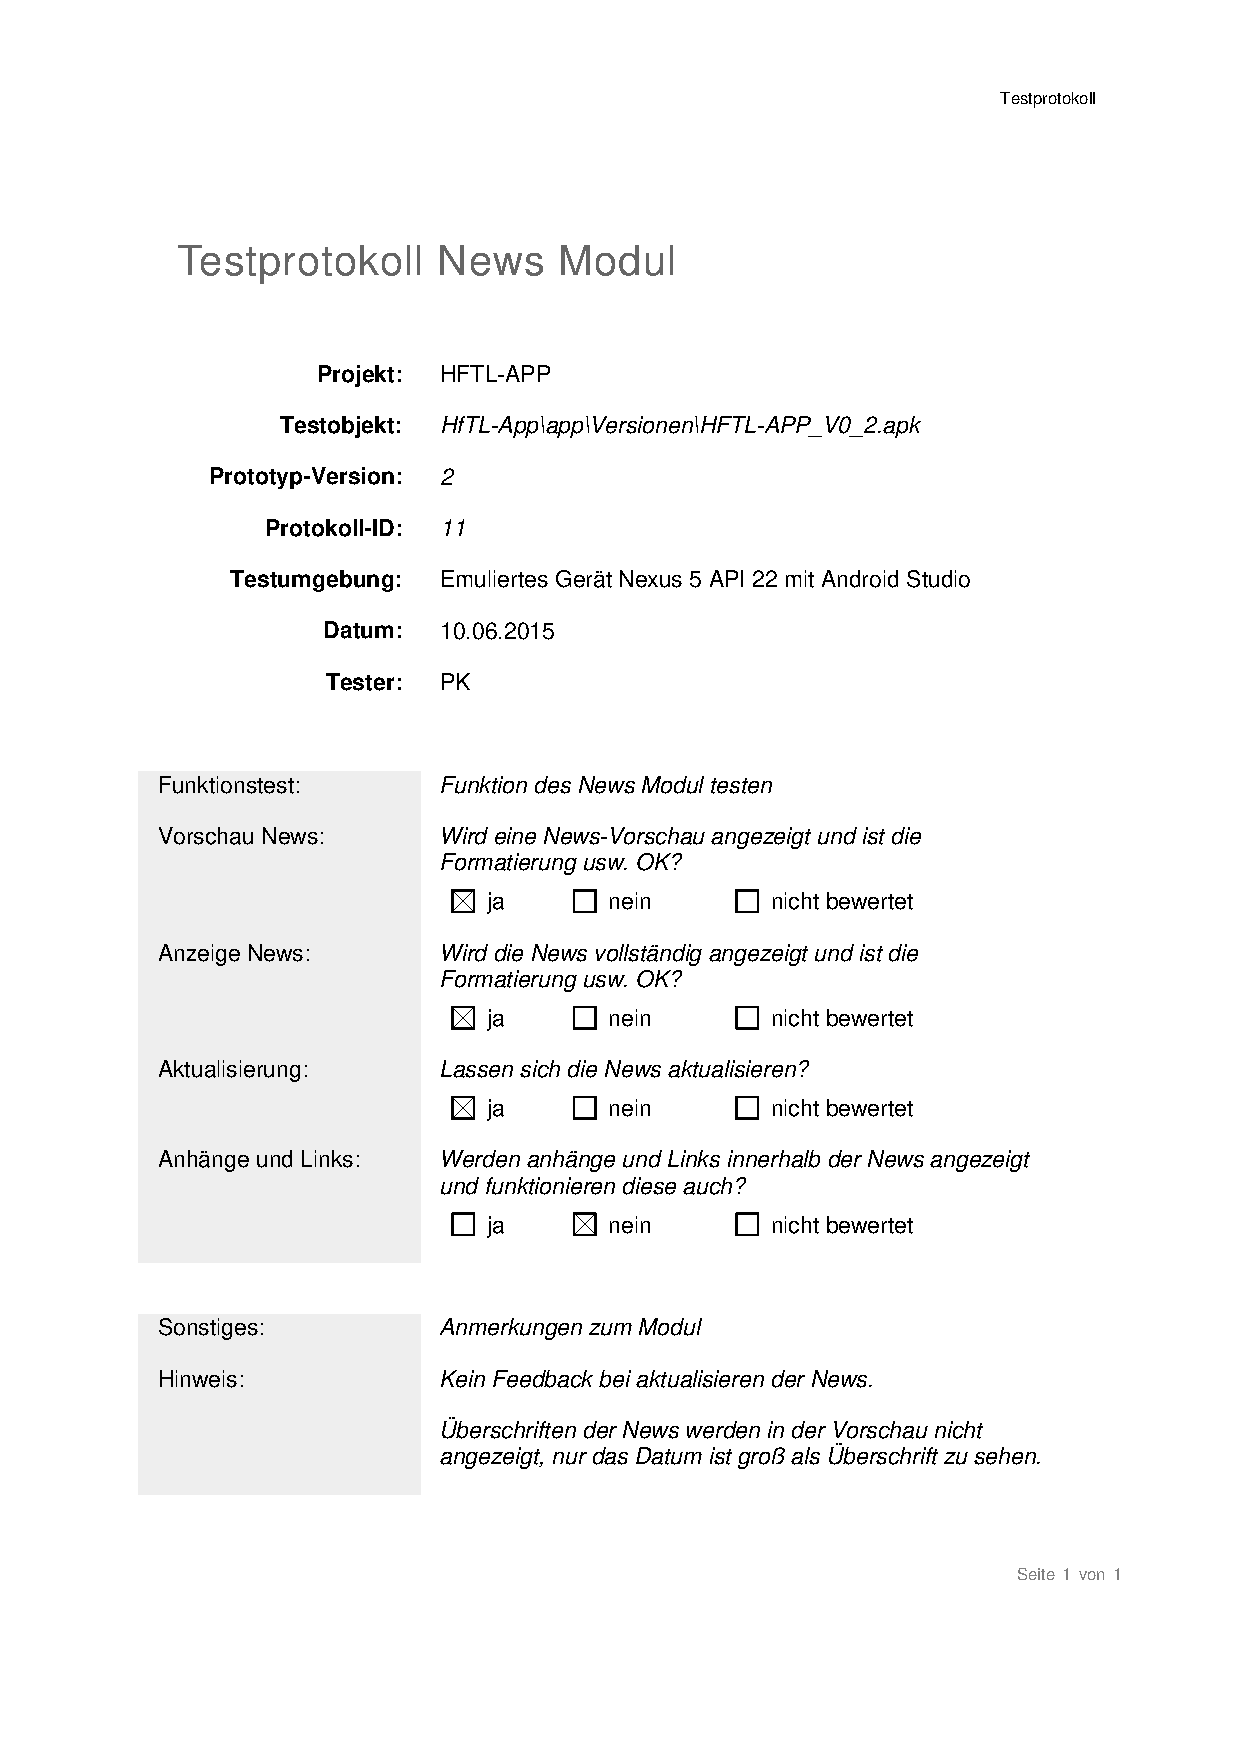
\includepdf[pages=-,noautoscale]{04_Anhang/files/Testprotokolle/News_Modul/10062015_Testprotokoll_News.pdf}

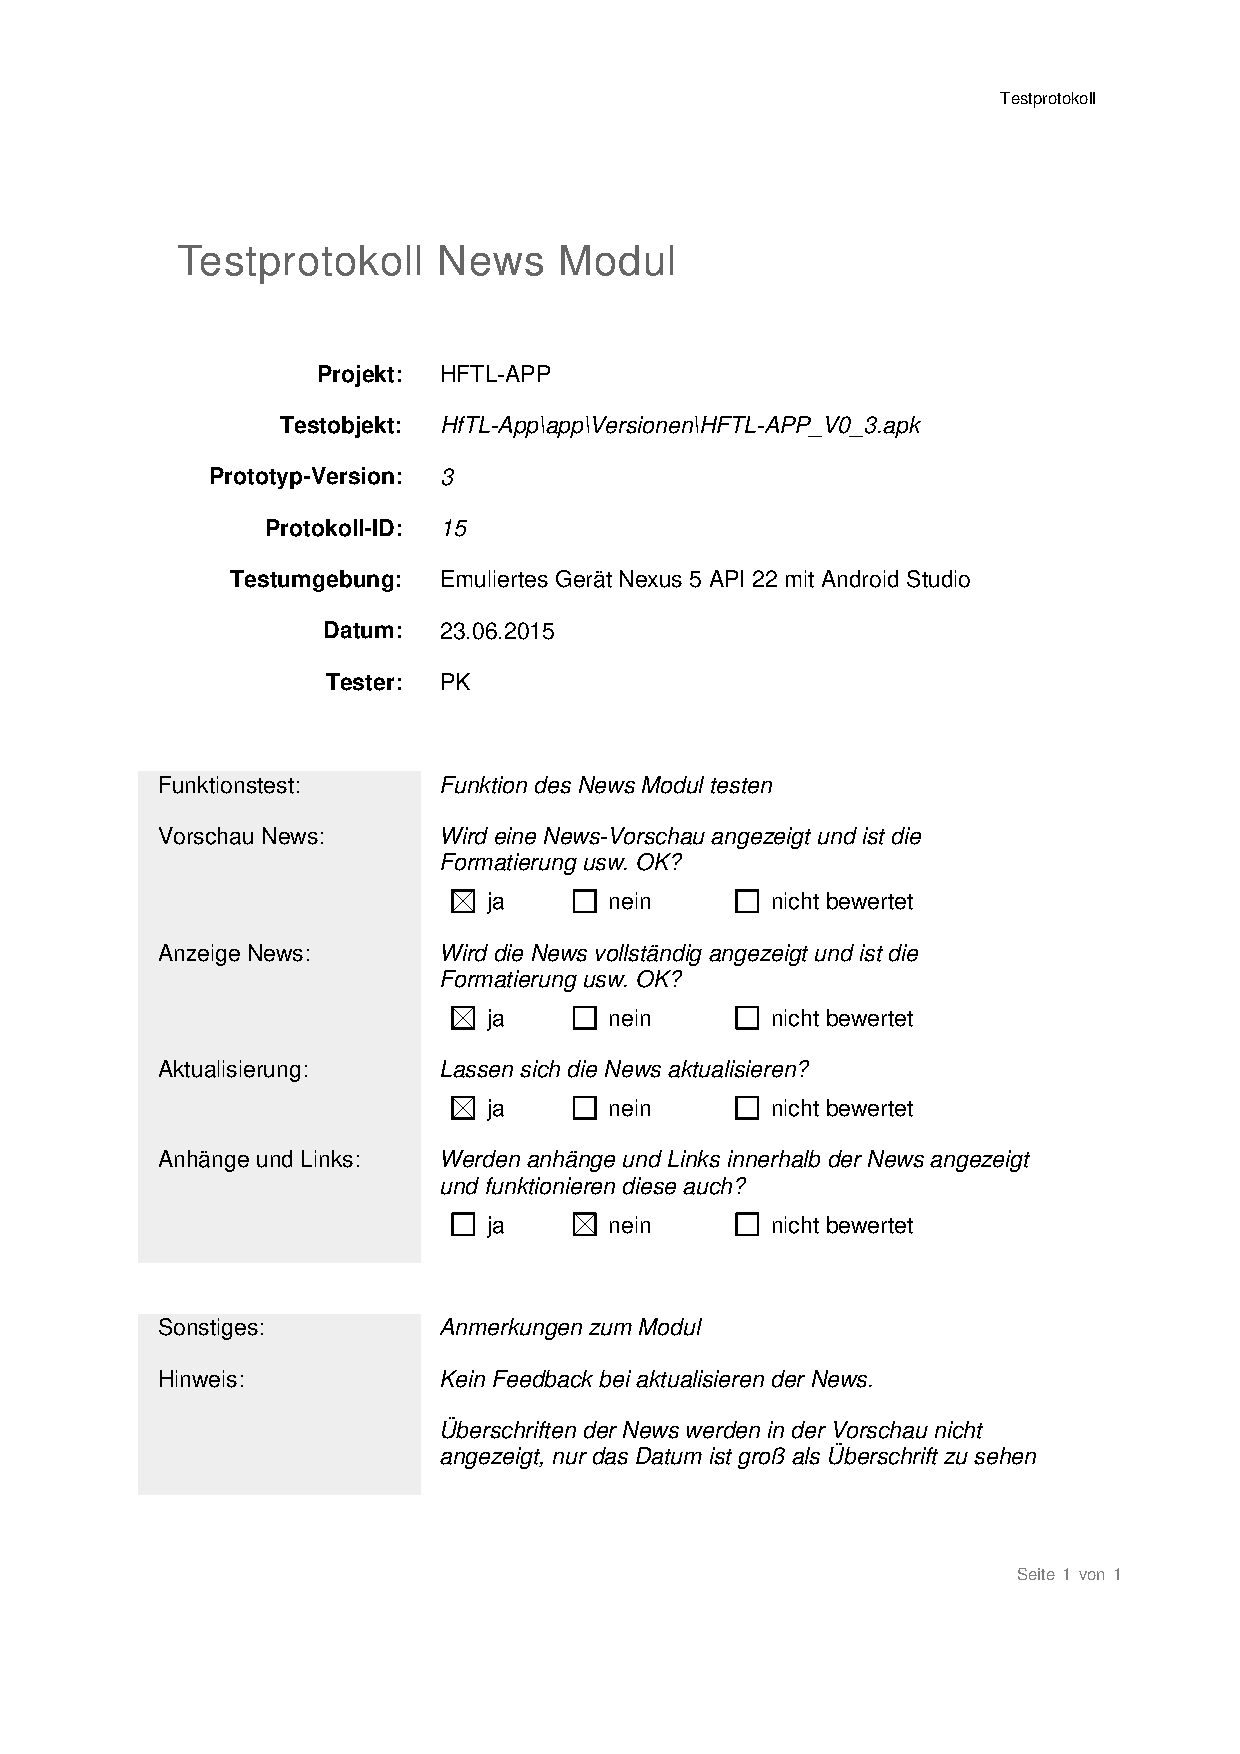
\includepdf[pages=-,noautoscale]{04_Anhang/files/Testprotokolle/News_Modul/23062015_Testprotokoll_News.pdf}

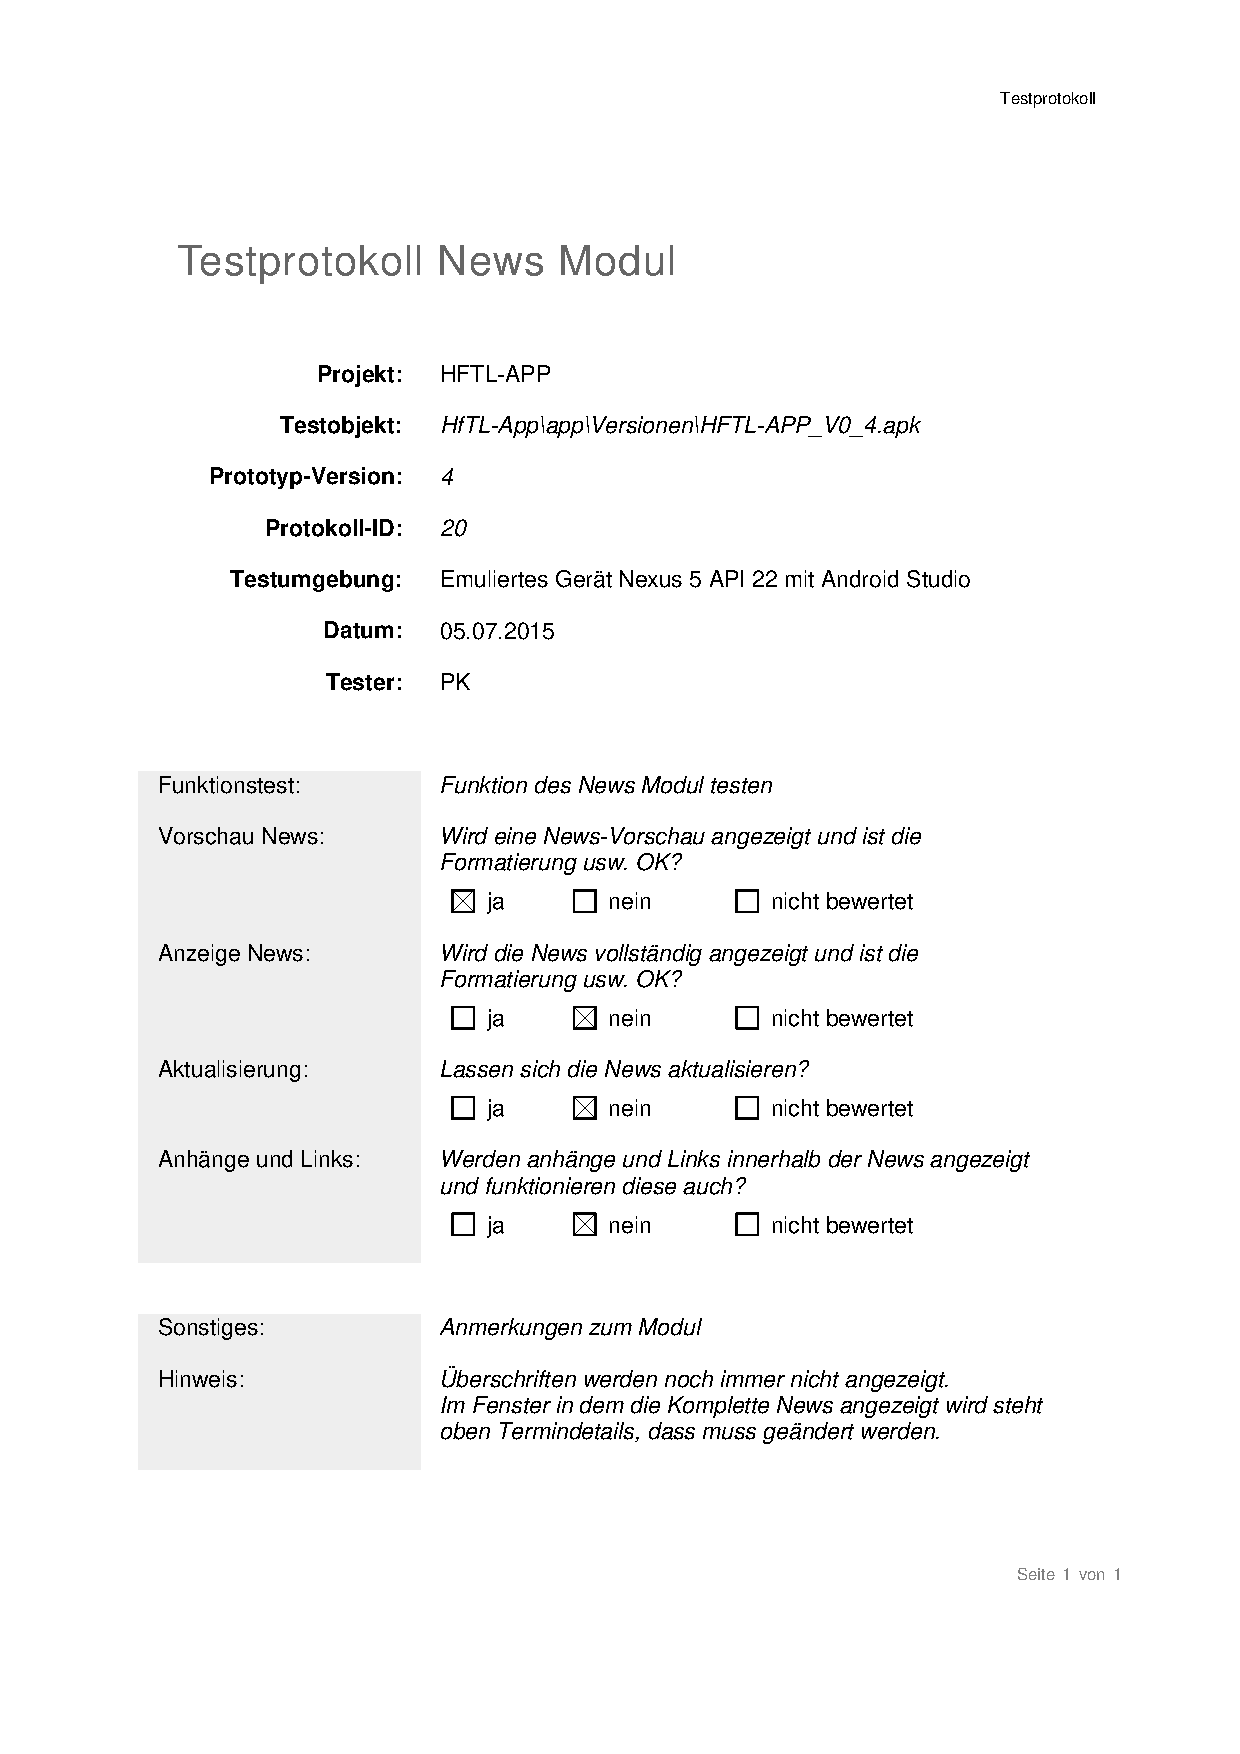
\includepdf[pages=-,noautoscale]{04_Anhang/files/Testprotokolle/News_Modul/05072015_Testprotokoll_News.pdf}

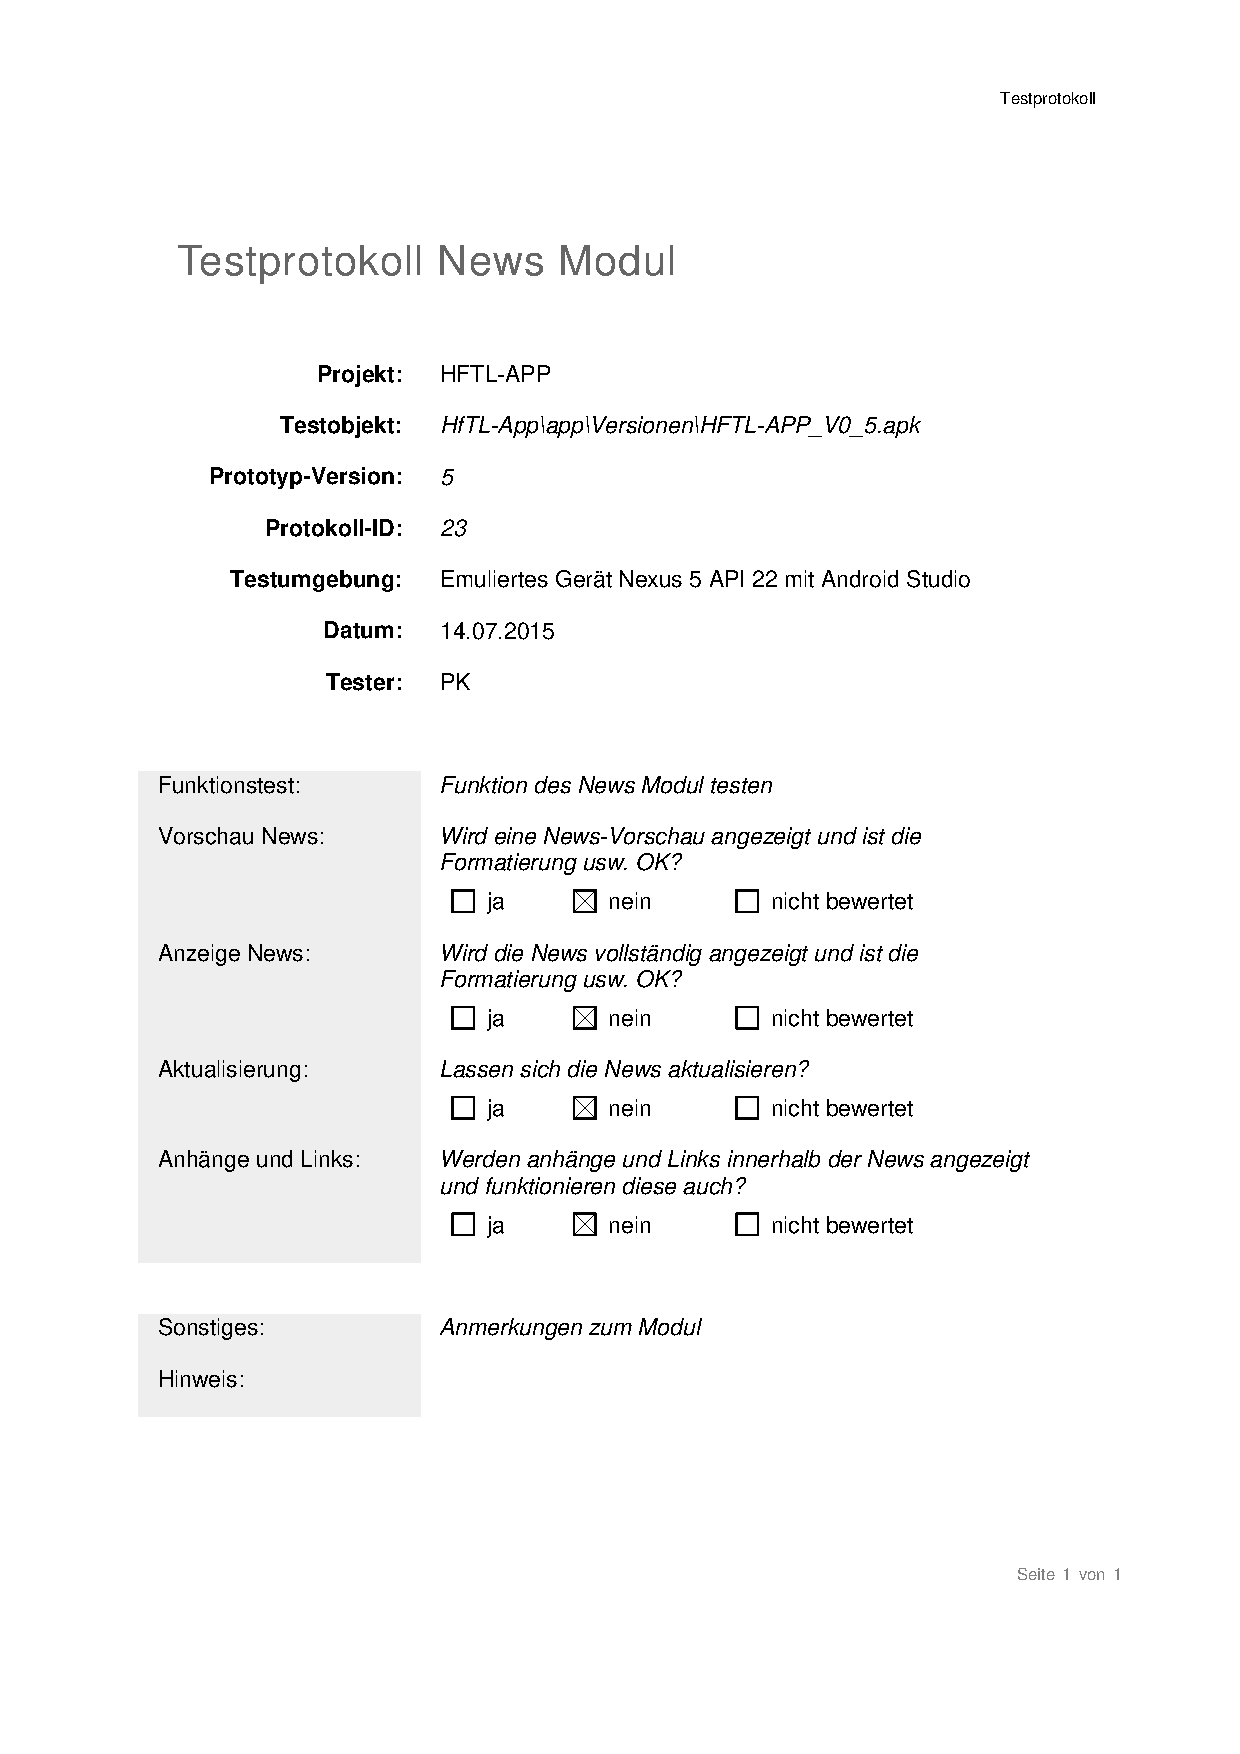
\includepdf[pages=-,noautoscale]{04_Anhang/files/Testprotokolle/News_Modul/14072015_Testprotokoll_News.pdf}
	
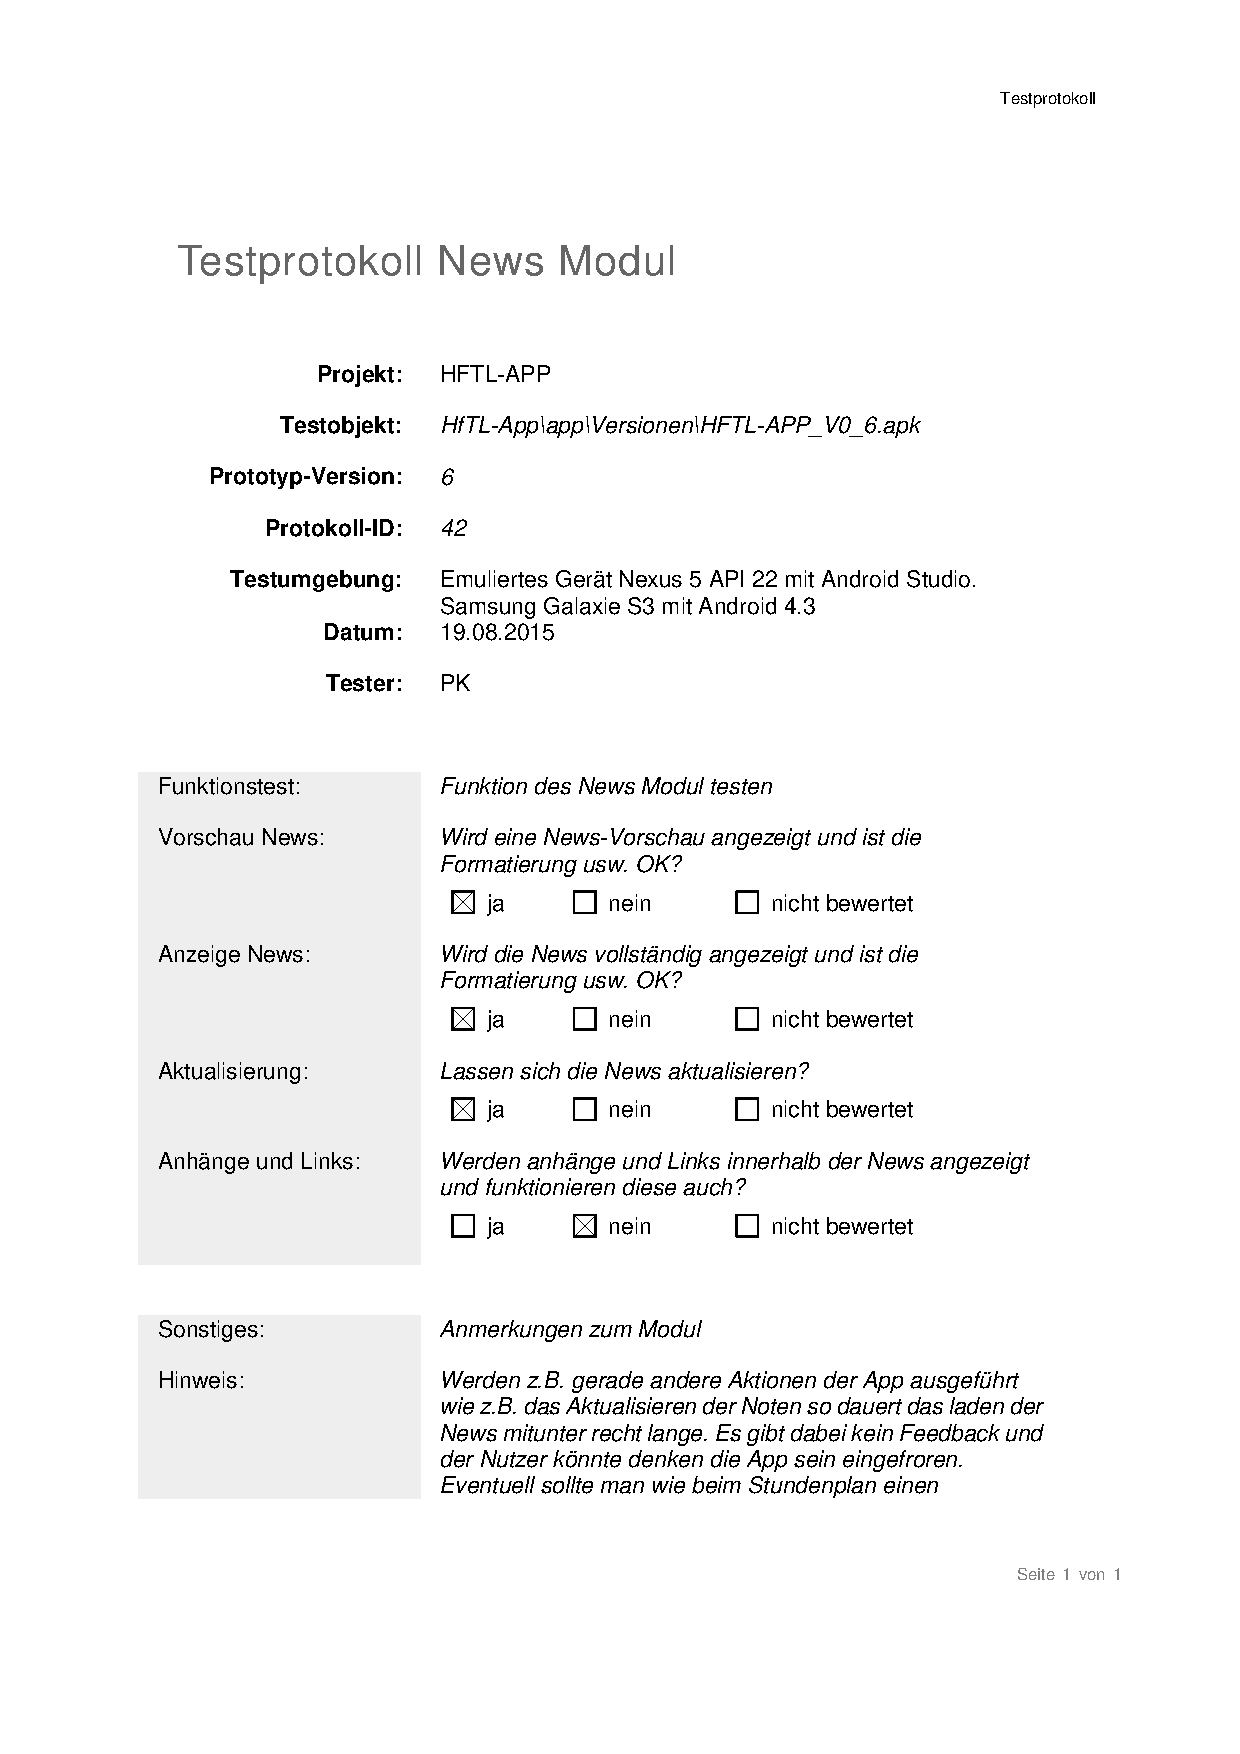
\includepdf[pages=-,noautoscale]{04_Anhang/files/Testprotokolle/News_Modul/19082015_Testprotokoll_News.pdf}

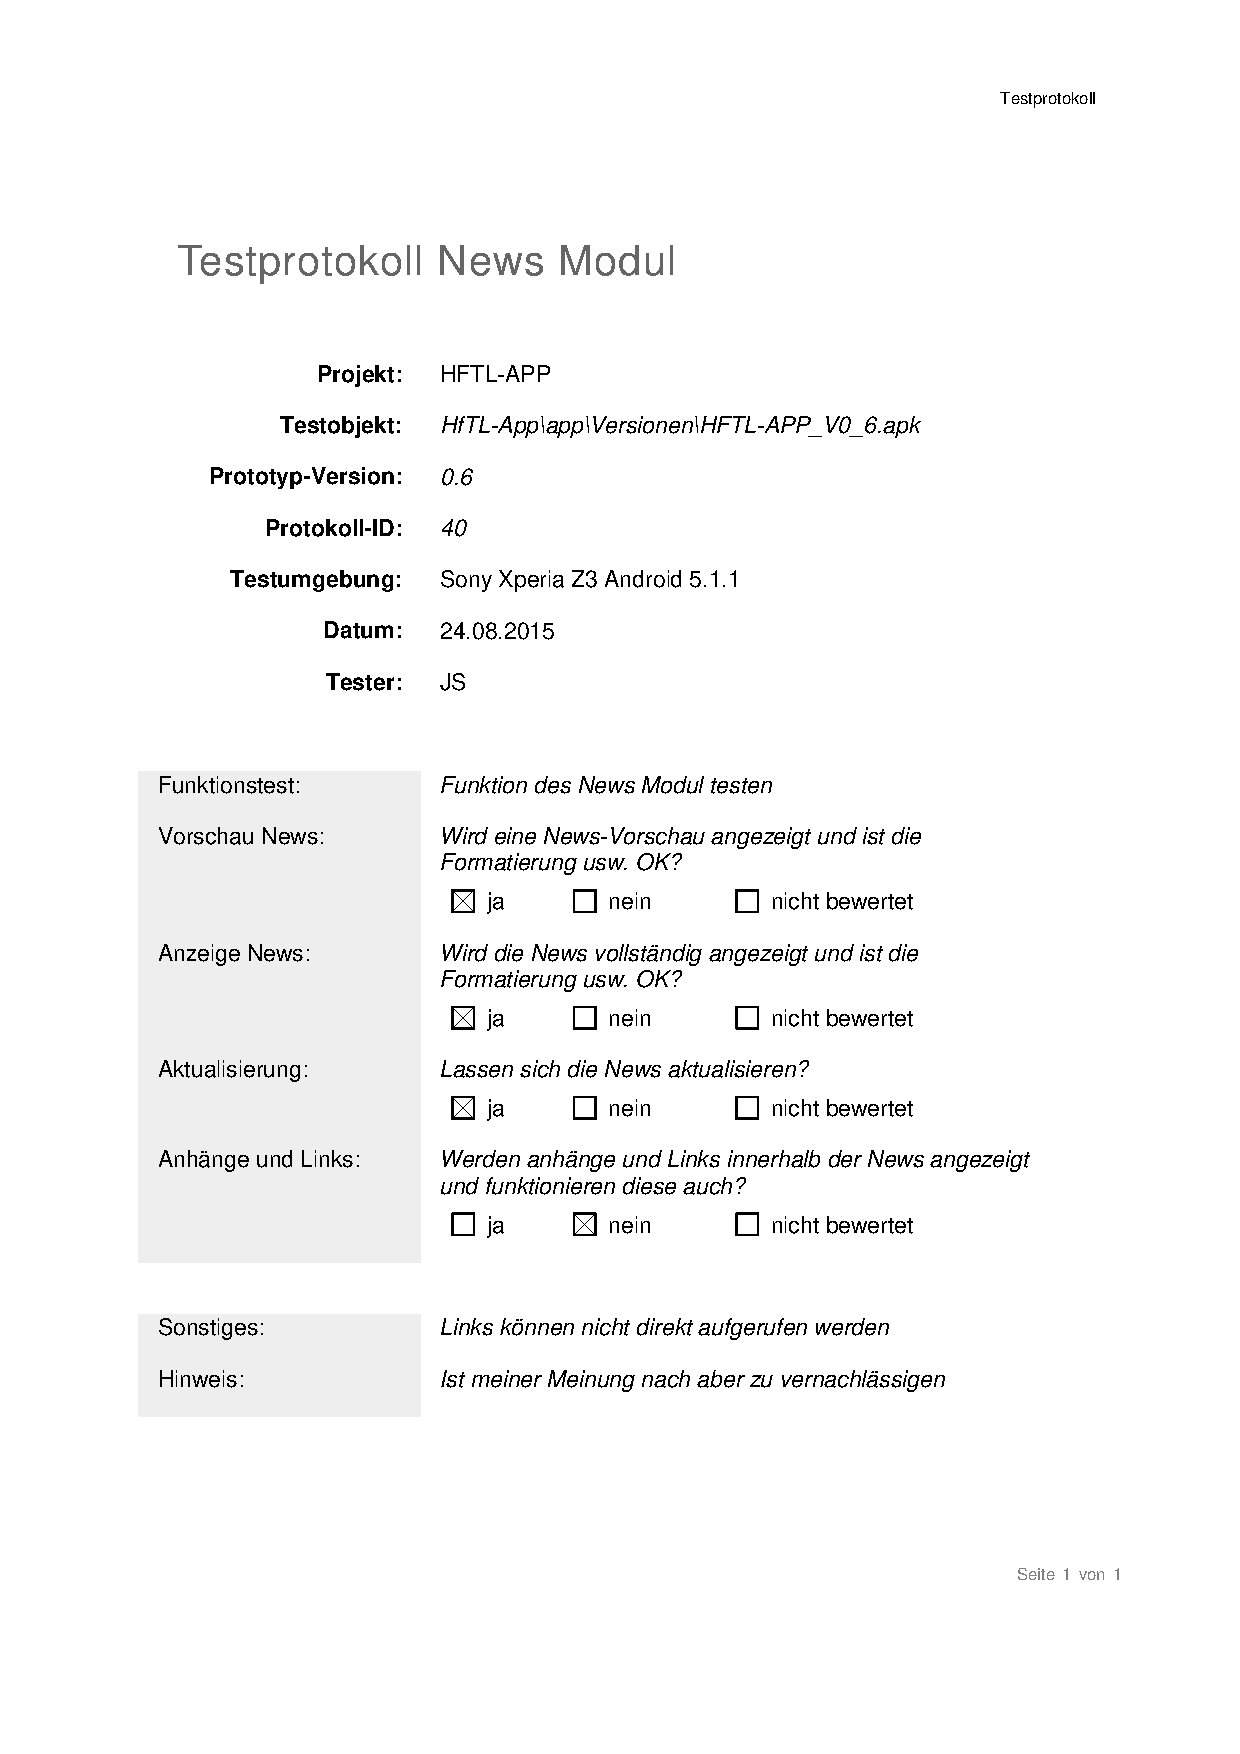
\includepdf[pages=-,noautoscale]{04_Anhang/files/Testprotokolle/News_Modul/24082015_Testprotokoll_News.pdf}

%%%%%%%%%%%%%%%%%%%%%%%%%%%%%%%%%%%%%%%%%%%%%%%%%%%%%%%%%%%%%%%

\Large{Testprotokolle zum Noten Modul}

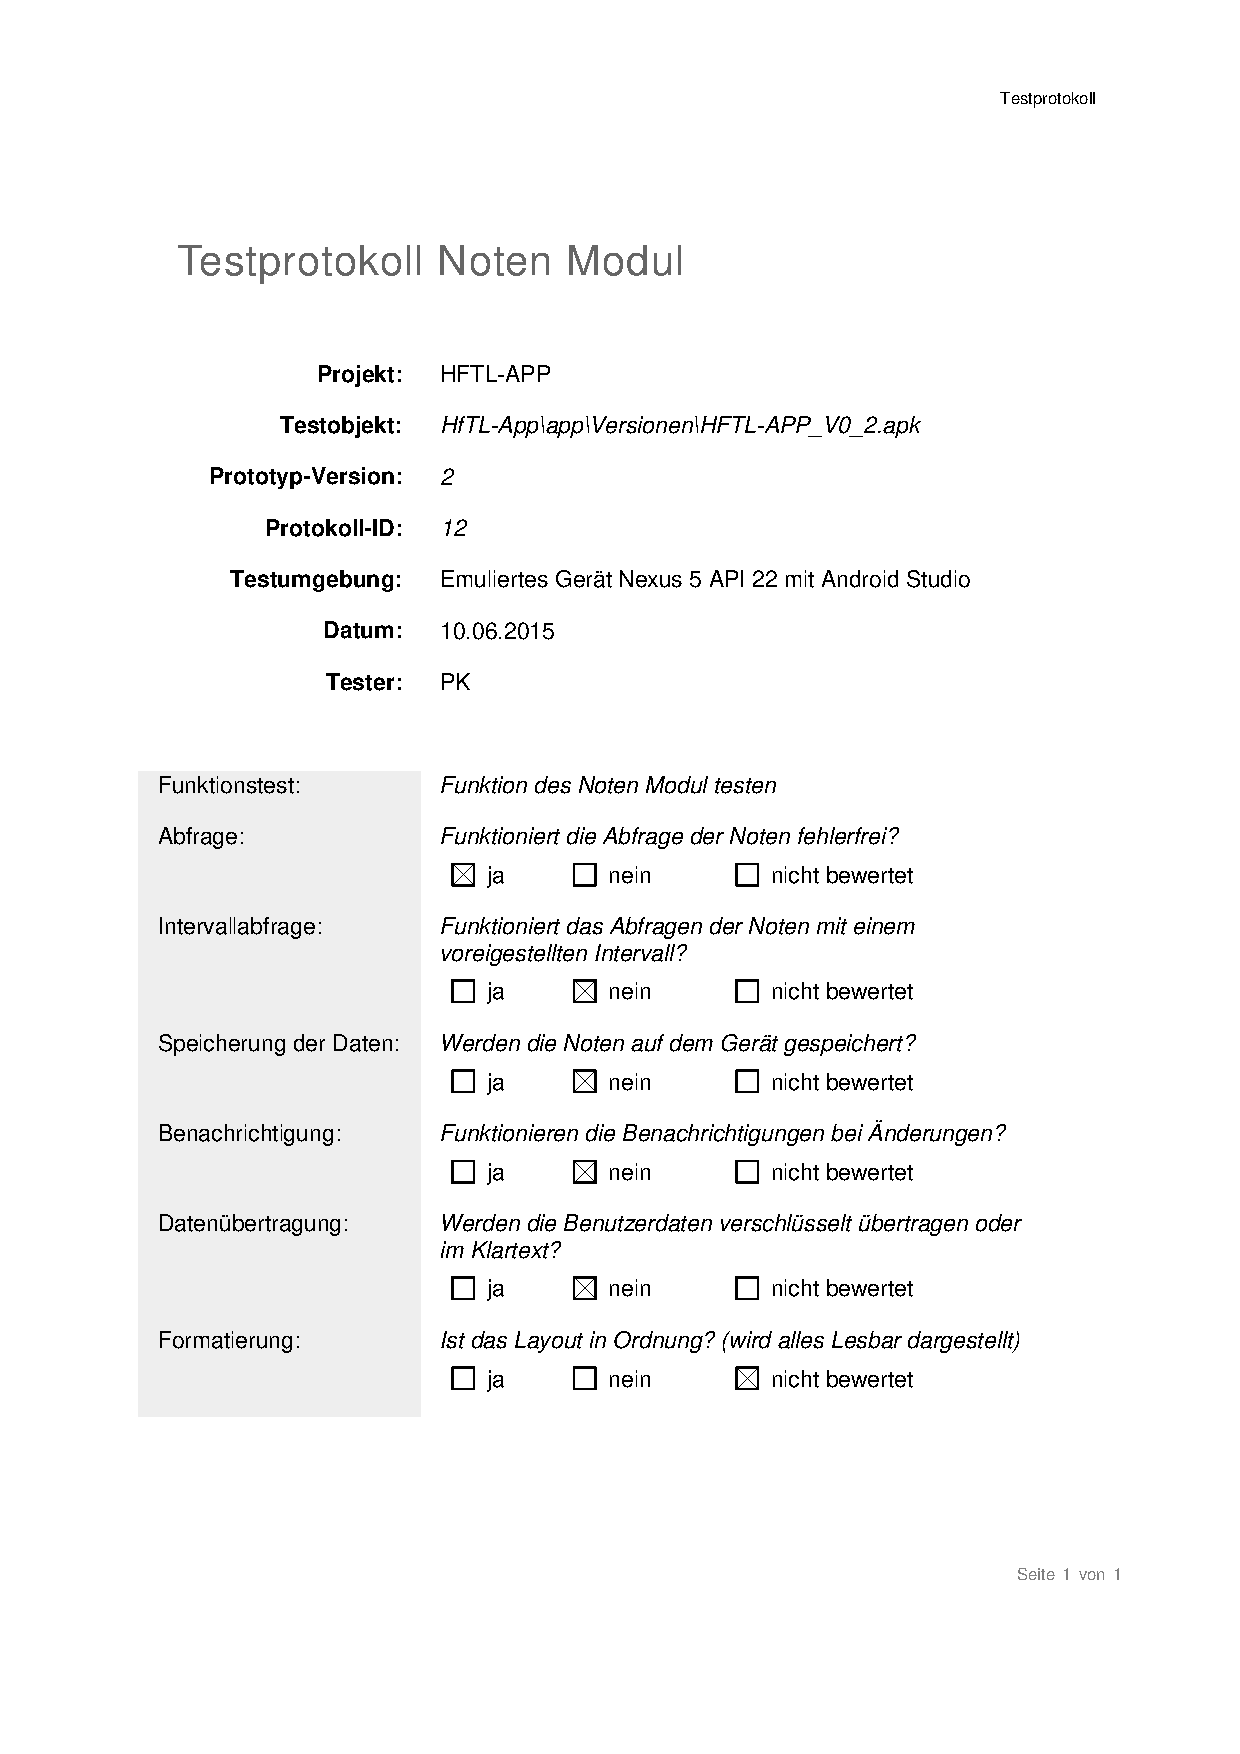
\includepdf[pages=-,noautoscale]{04_Anhang/files/Testprotokolle/Noten_Modul/10062015_Testprotokoll_Noten.pdf}

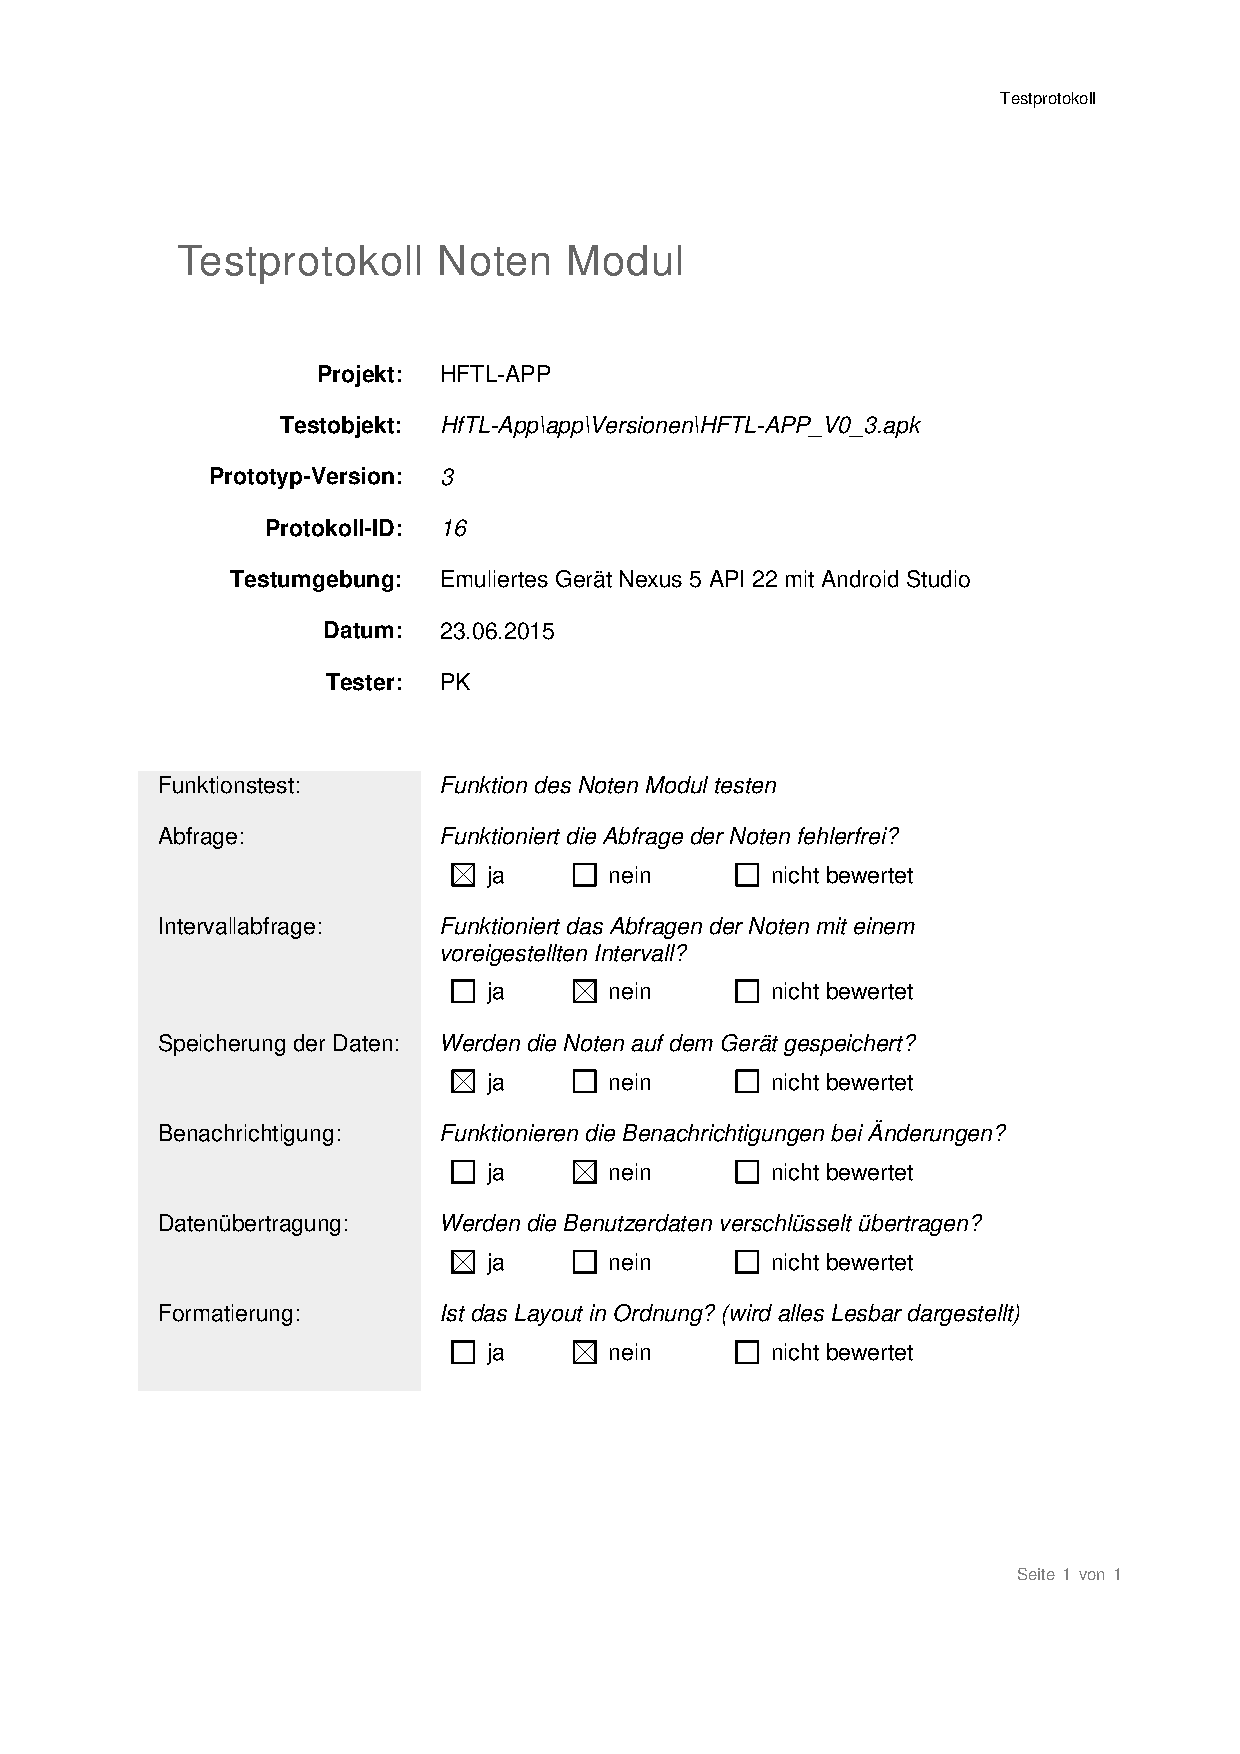
\includepdf[pages=-,noautoscale]{04_Anhang/files/Testprotokolle/Noten_Modul/23062015_Testprotokoll_Noten.pdf}

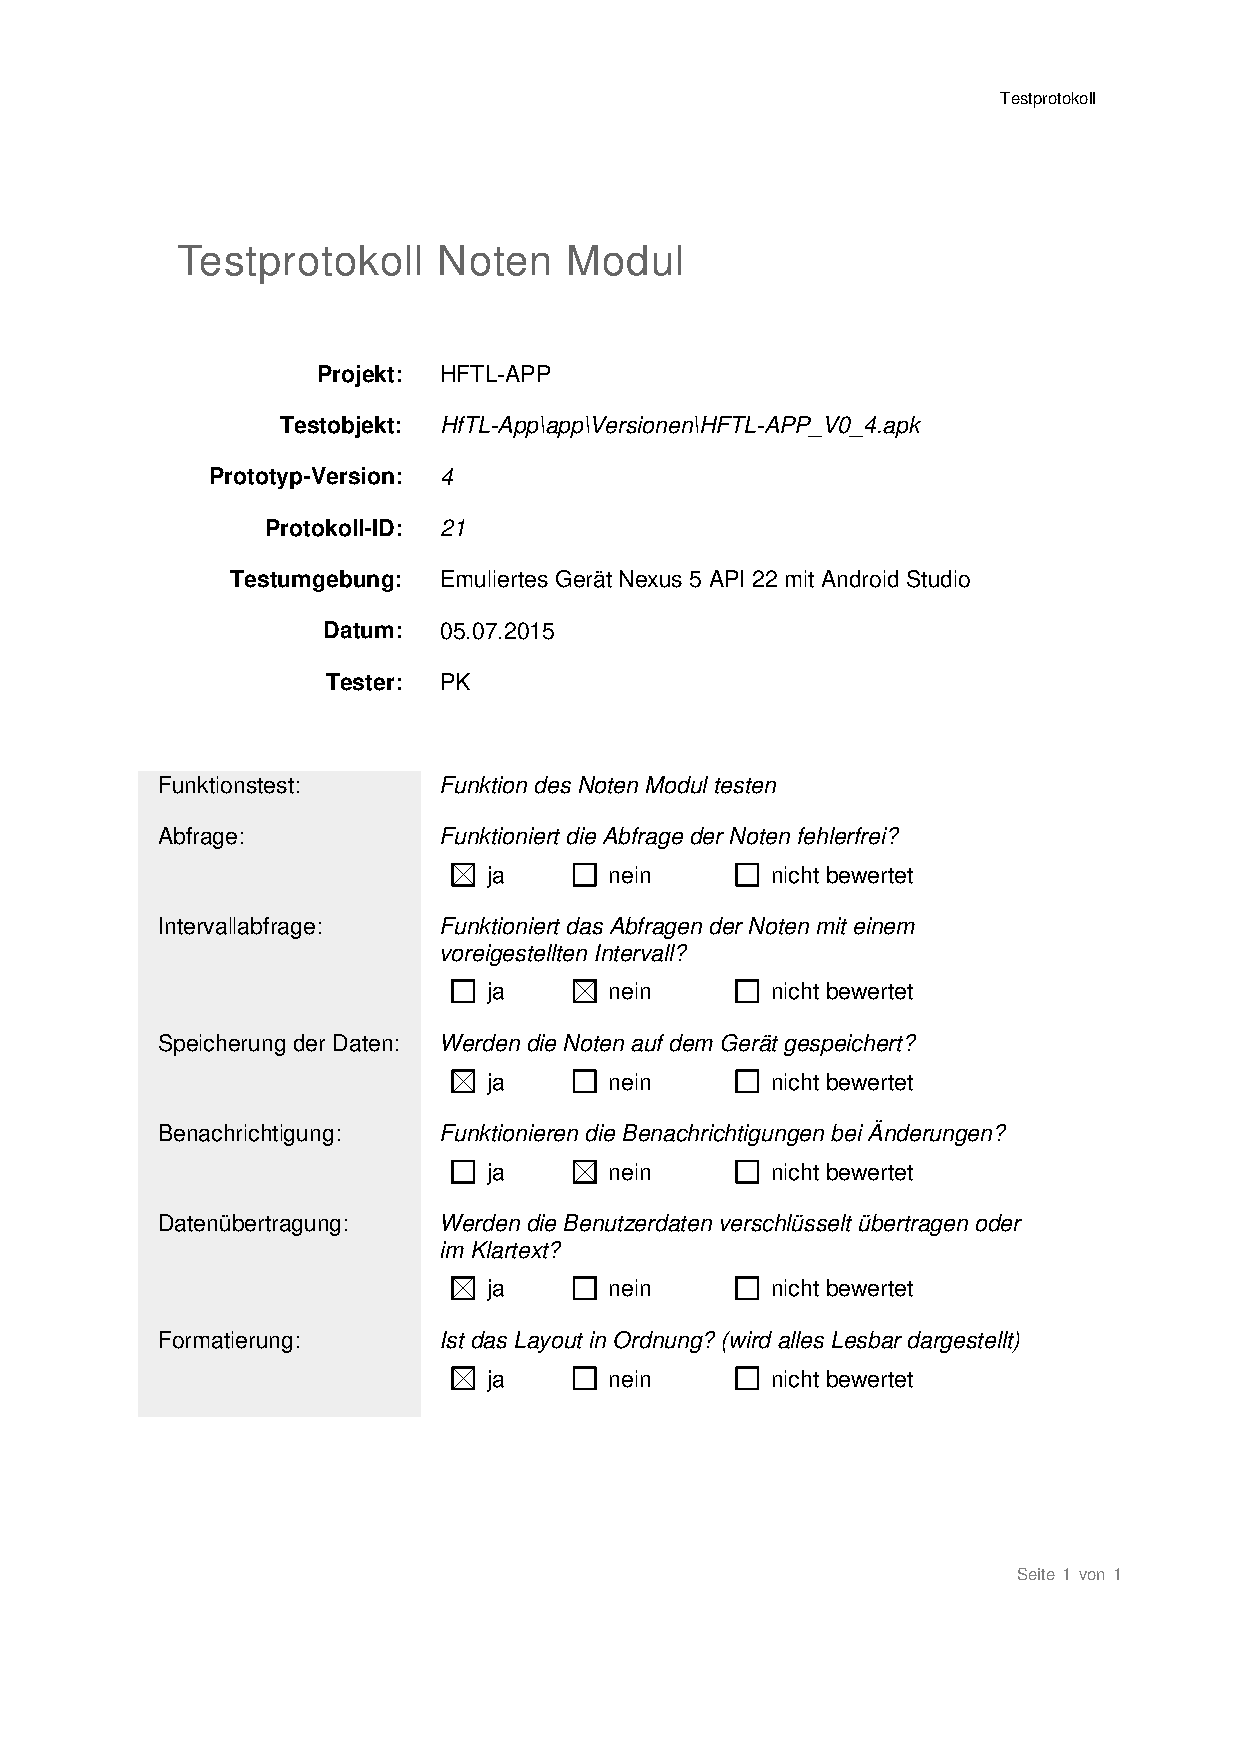
\includepdf[pages=-,noautoscale]{04_Anhang/files/Testprotokolle/Noten_Modul/05072015_Testprotokoll_Noten.pdf}

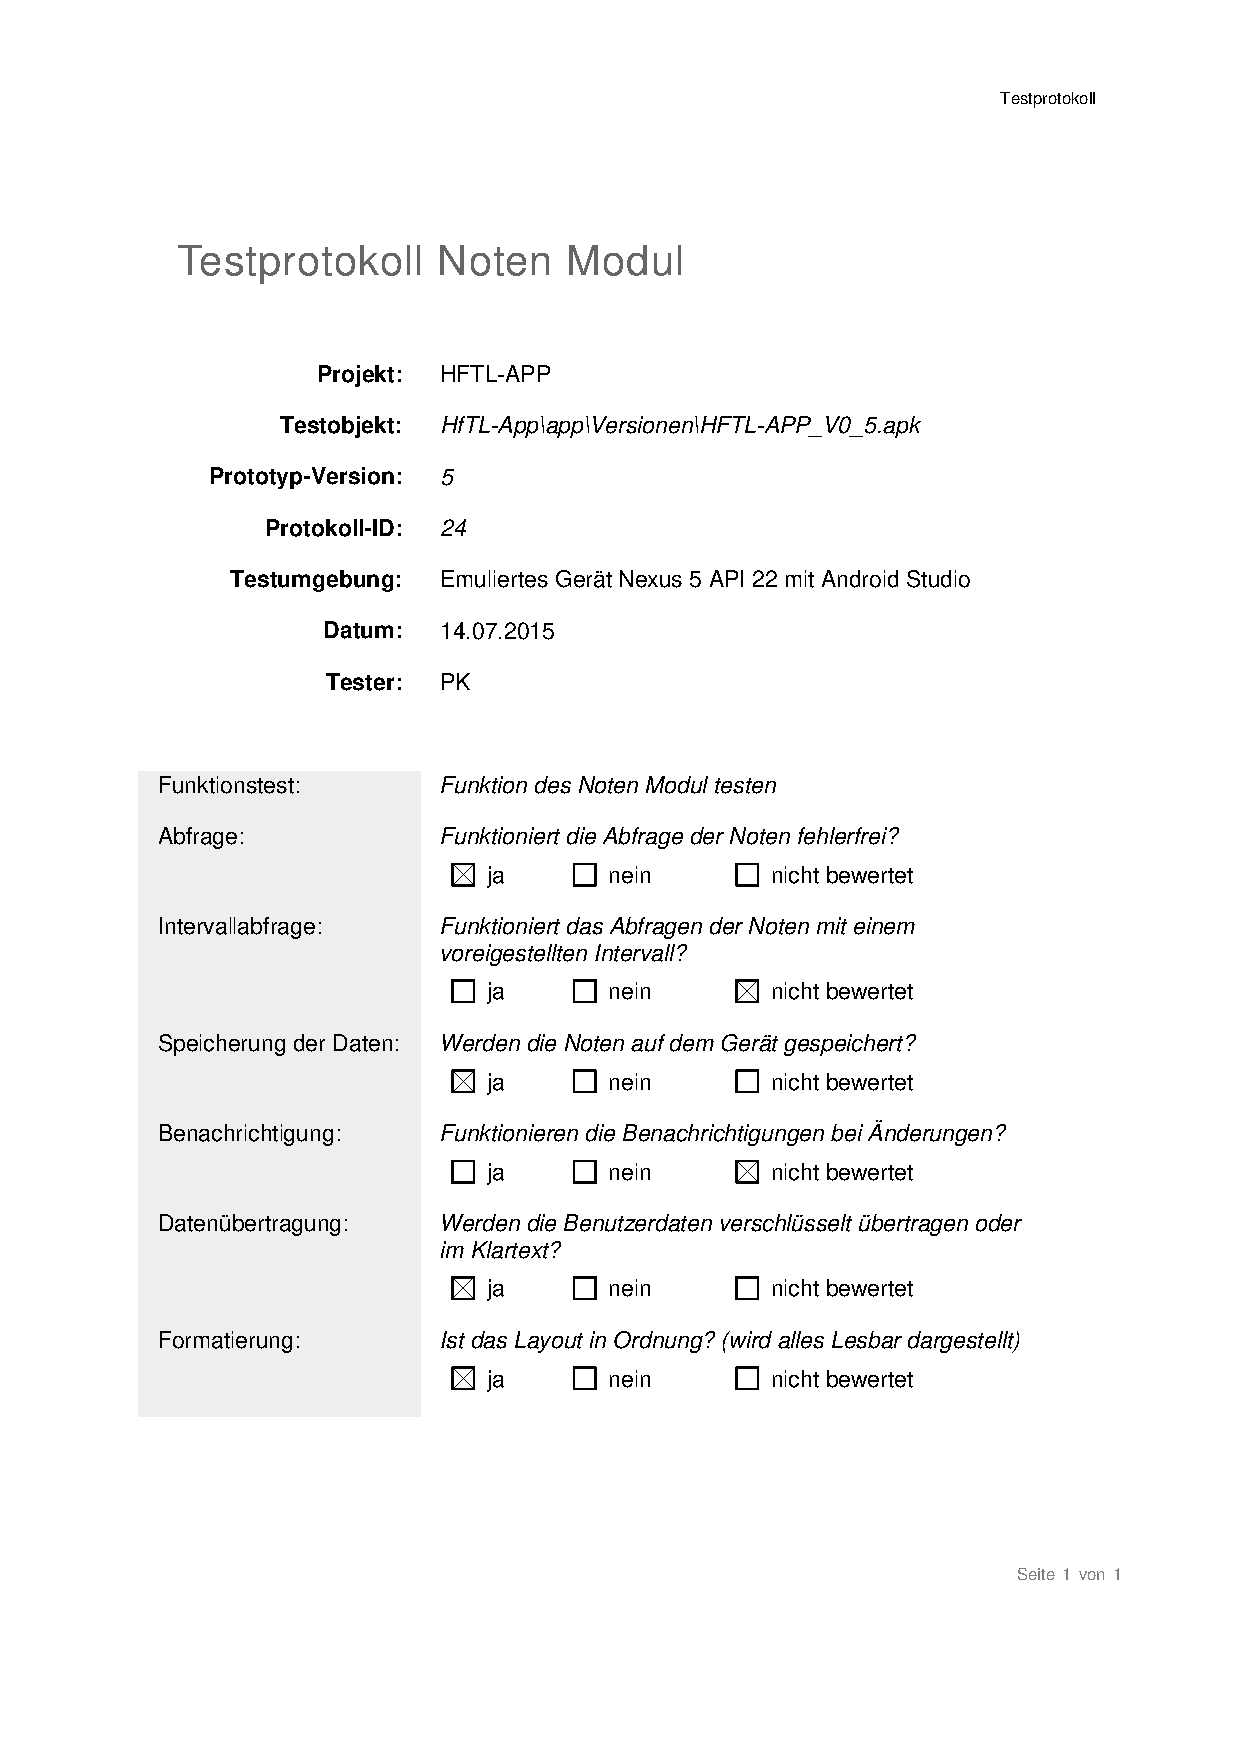
\includepdf[pages=-,noautoscale]{04_Anhang/files/Testprotokolle/Noten_Modul/14072015_Testprotokoll_Noten.pdf}

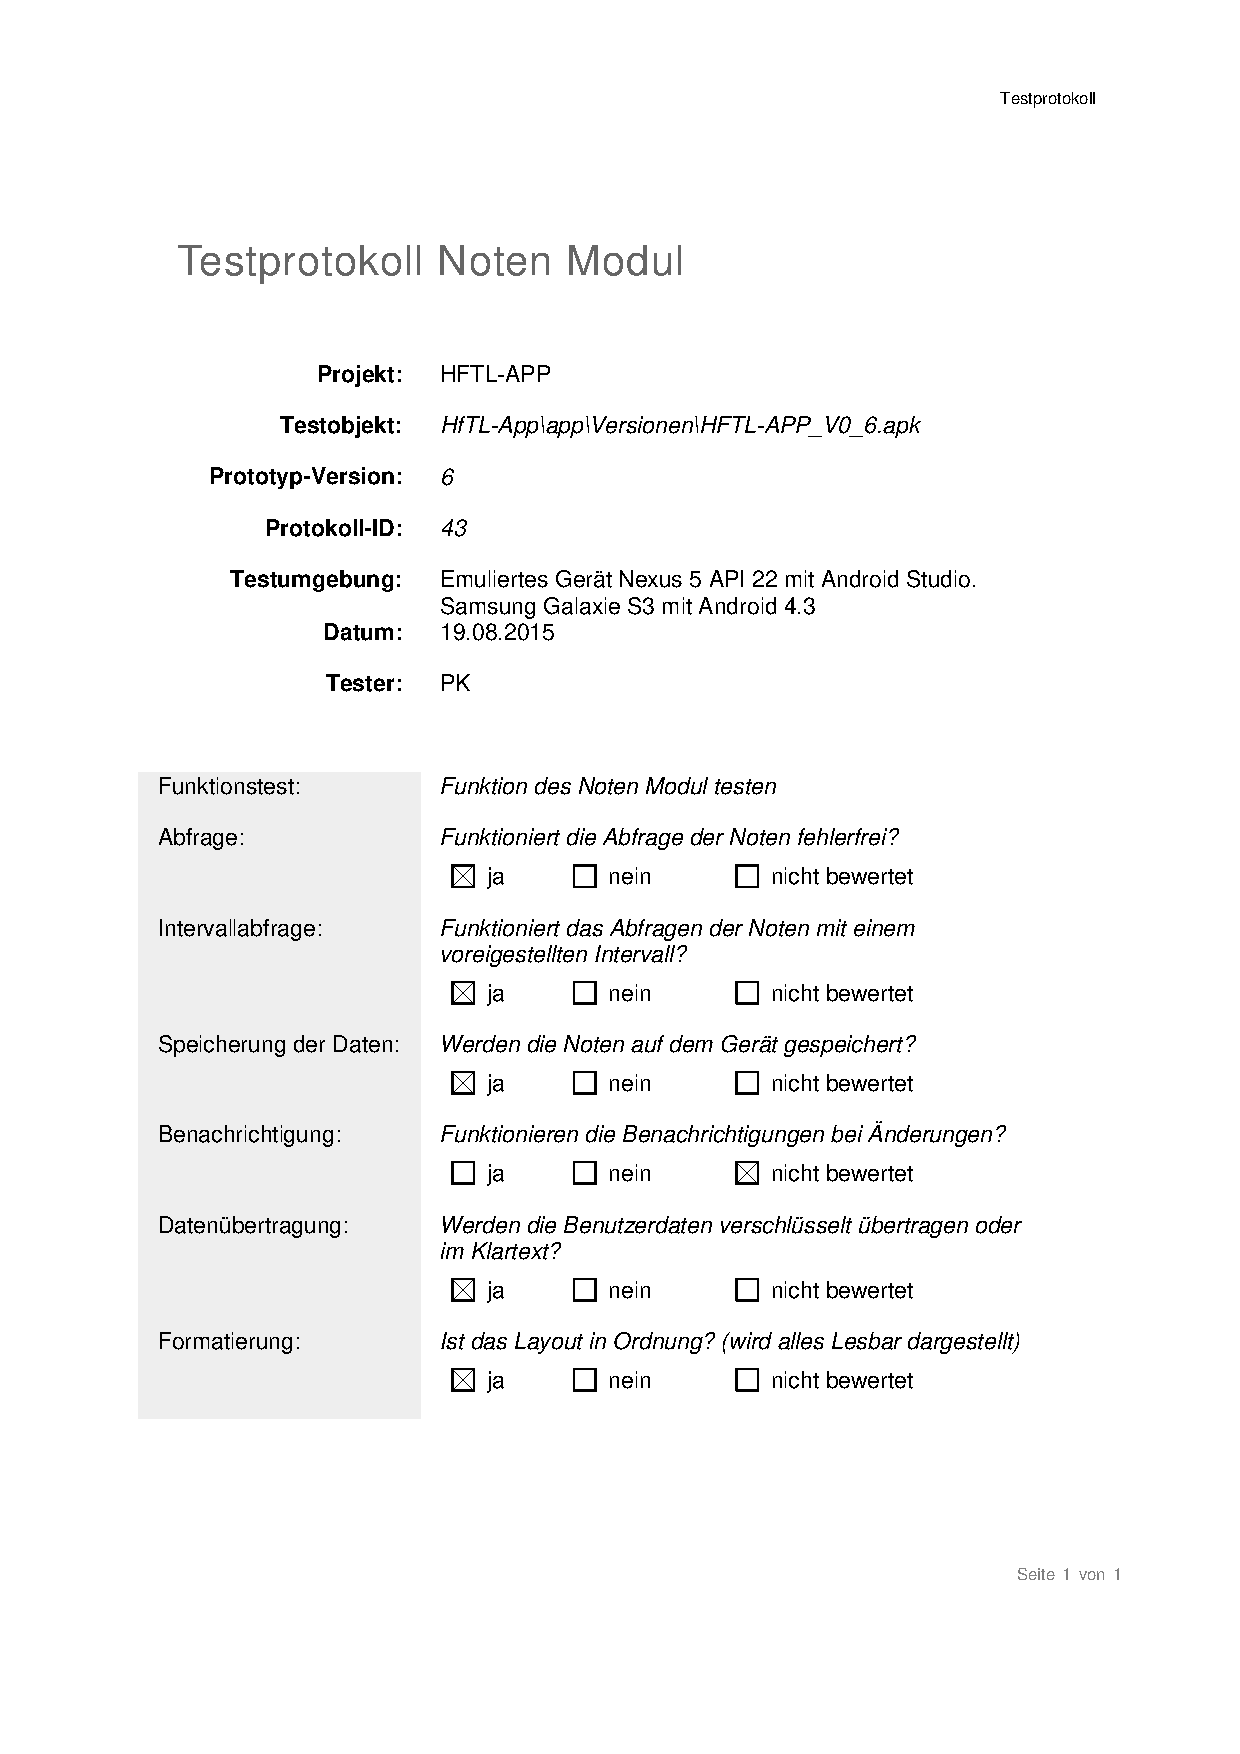
\includepdf[pages=-,noautoscale]{04_Anhang/files/Testprotokolle/Noten_Modul/19082015_Testprotokoll_Noten.pdf}

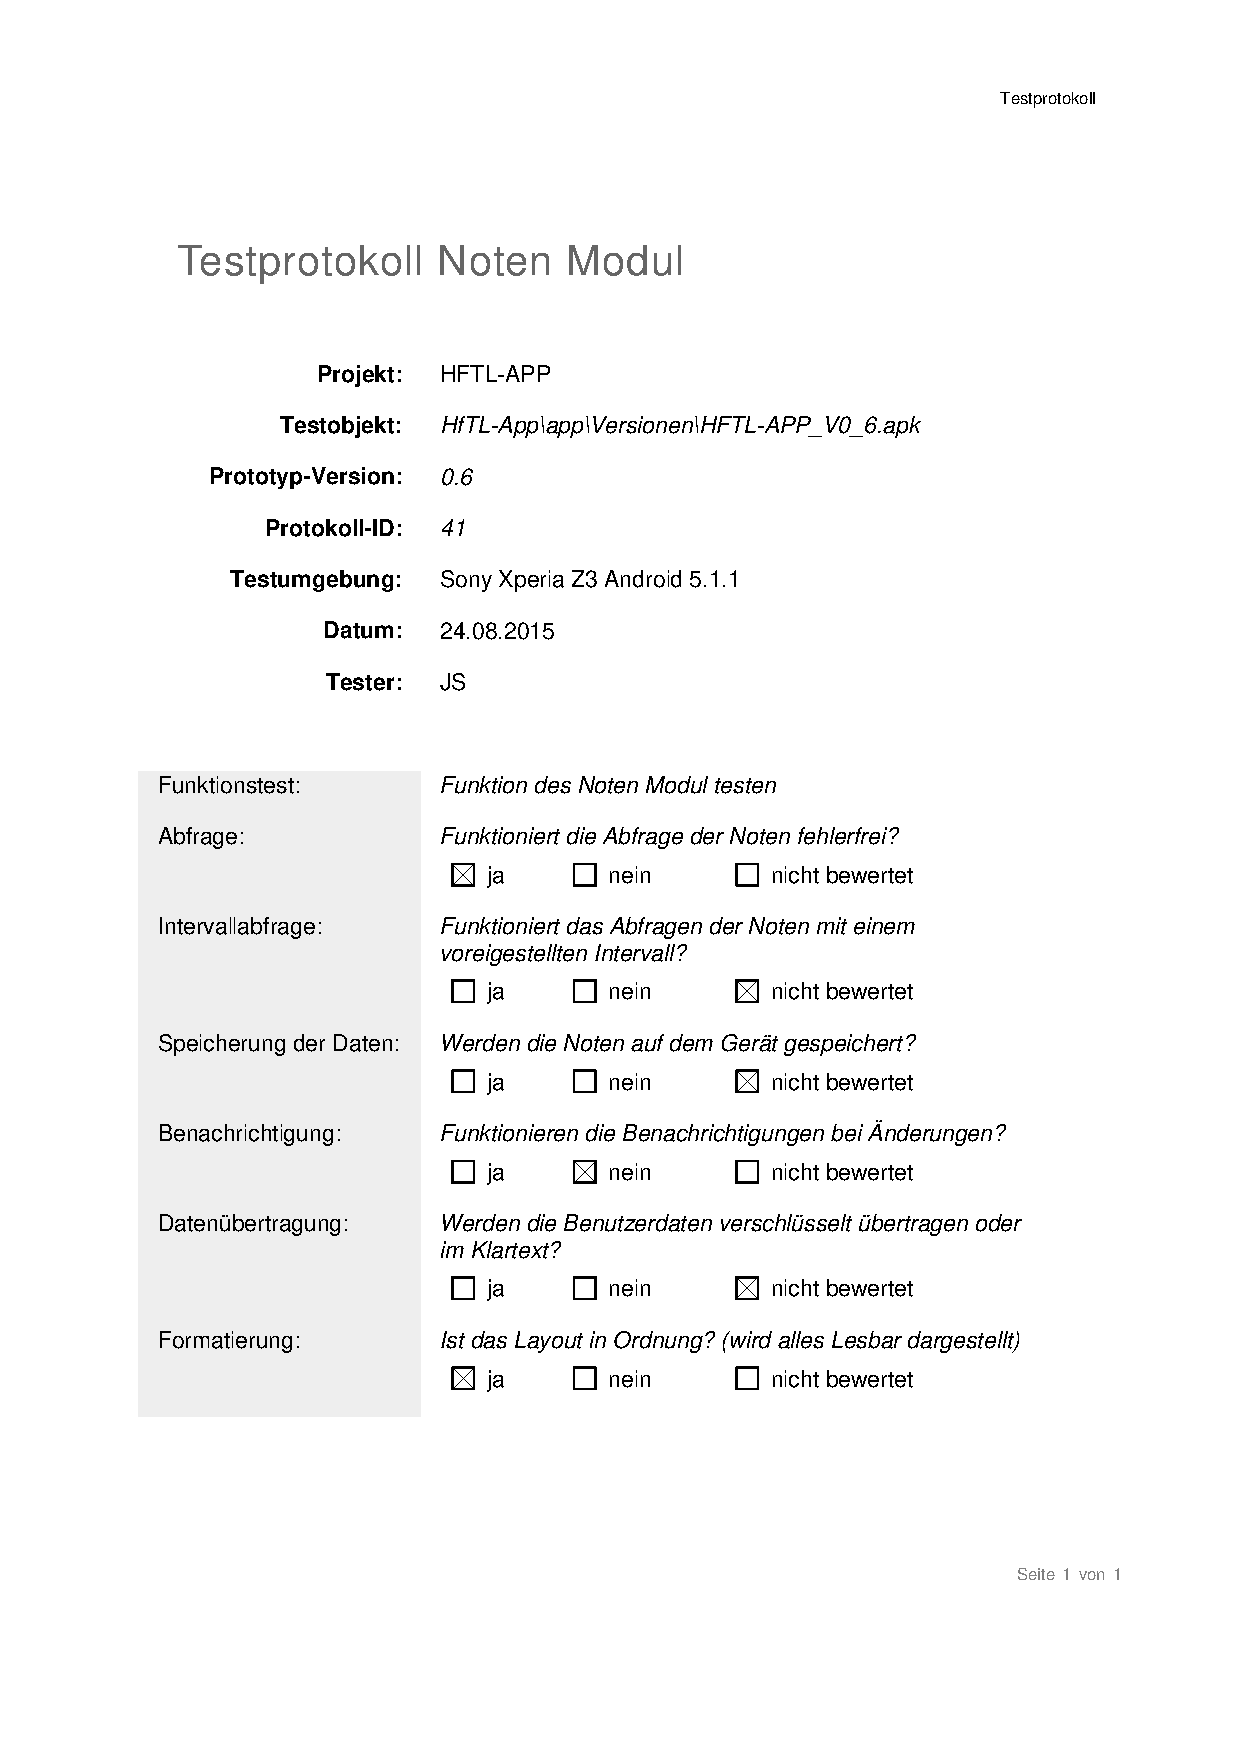
\includepdf[pages=-,noautoscale]{04_Anhang/files/Testprotokolle/Noten_Modul/24082015_Testprotokoll_Noten.pdf}


%%%%%%%%%%%%%%%%%%%%%%%%%%%%%%%%%%%%%%%%%%%%%%%%%%%%%%%%%%%%%%%%%%

\Large{Testprotokolle zum Stundenplan Modul}

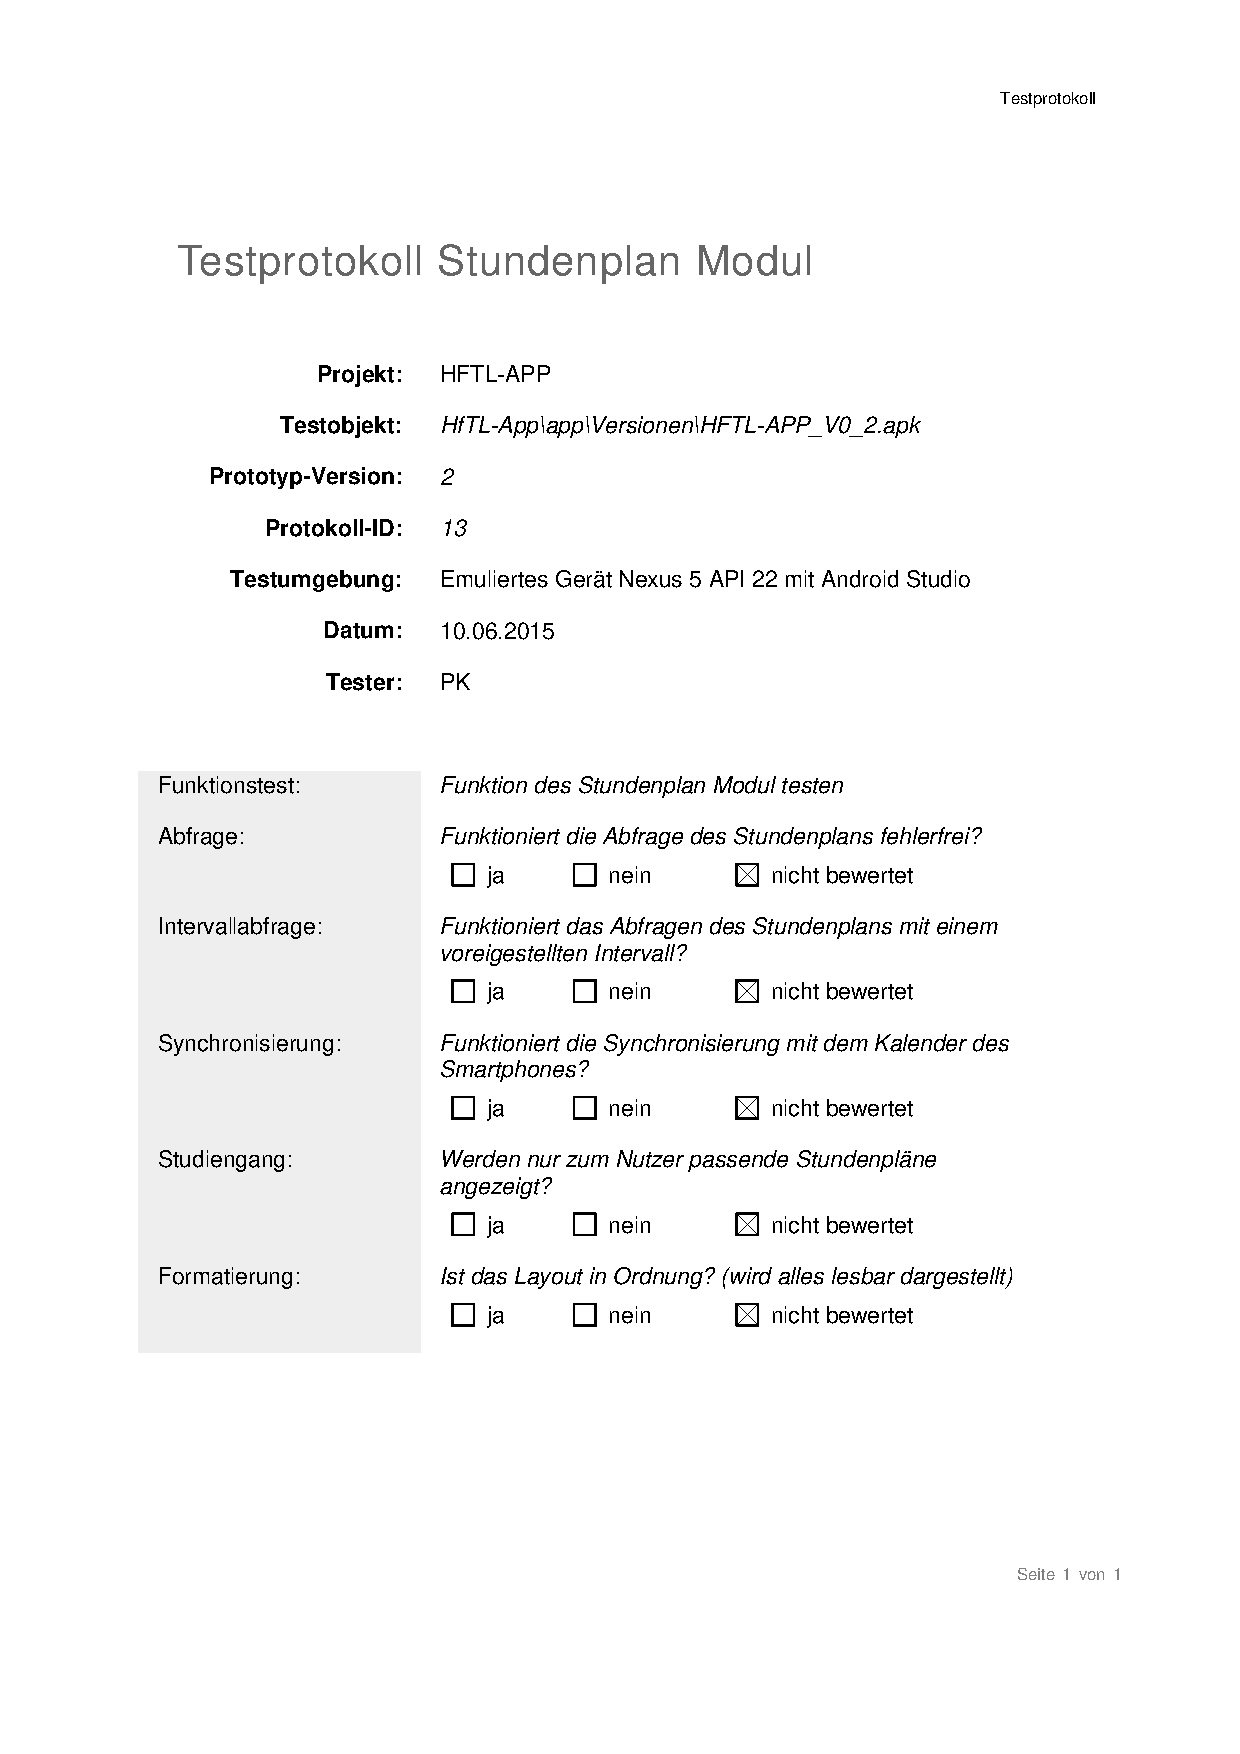
\includepdf[pages=-,noautoscale]{04_Anhang/files/Testprotokolle/Stundenplan_Modul/10062015_Testprotokoll_Stundenplan.pdf}

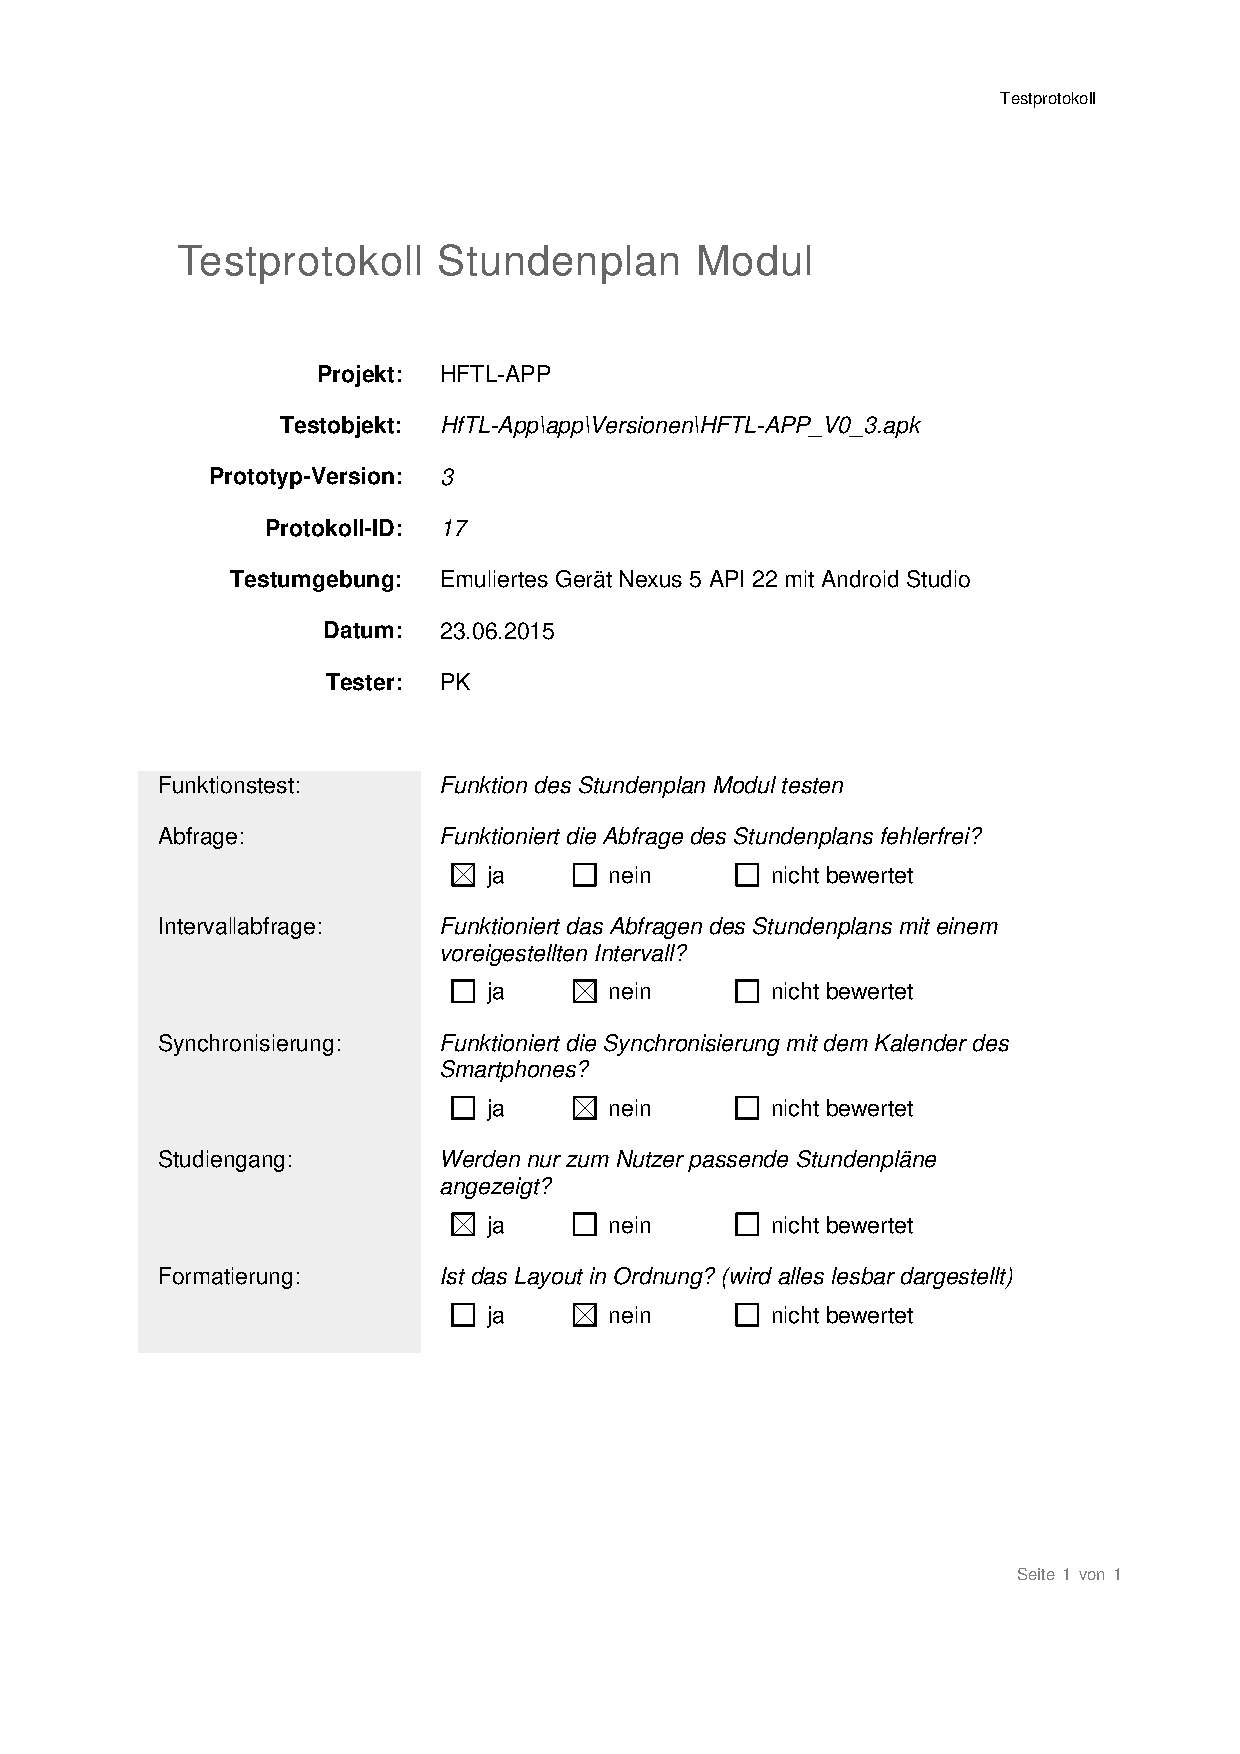
\includepdf[pages=-,noautoscale]{04_Anhang/files/Testprotokolle/Stundenplan_Modul/23062015_Testprotokoll_Stundenplan.pdf}

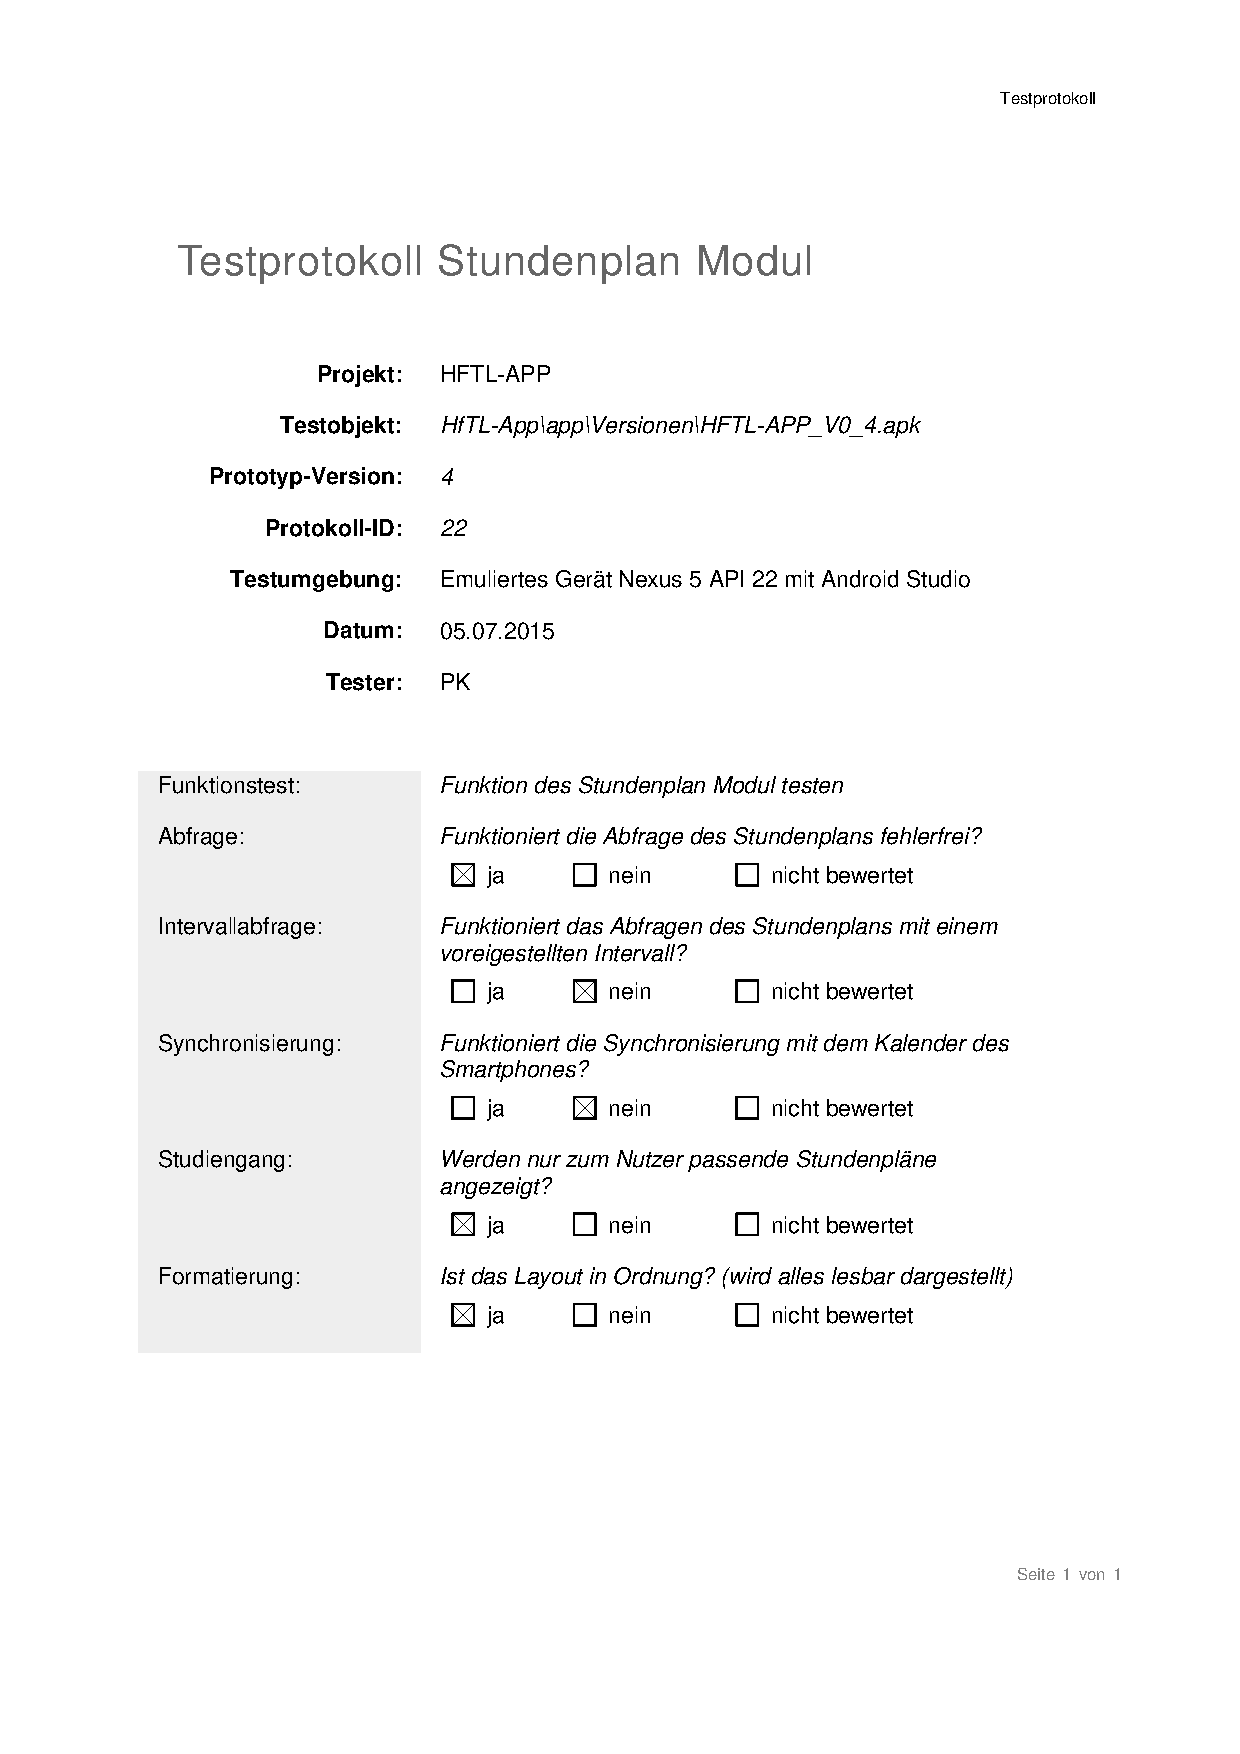
\includepdf[pages=-,noautoscale]{04_Anhang/files/Testprotokolle/Stundenplan_Modul/05072015_Testprotokoll_Stundenplan.pdf}

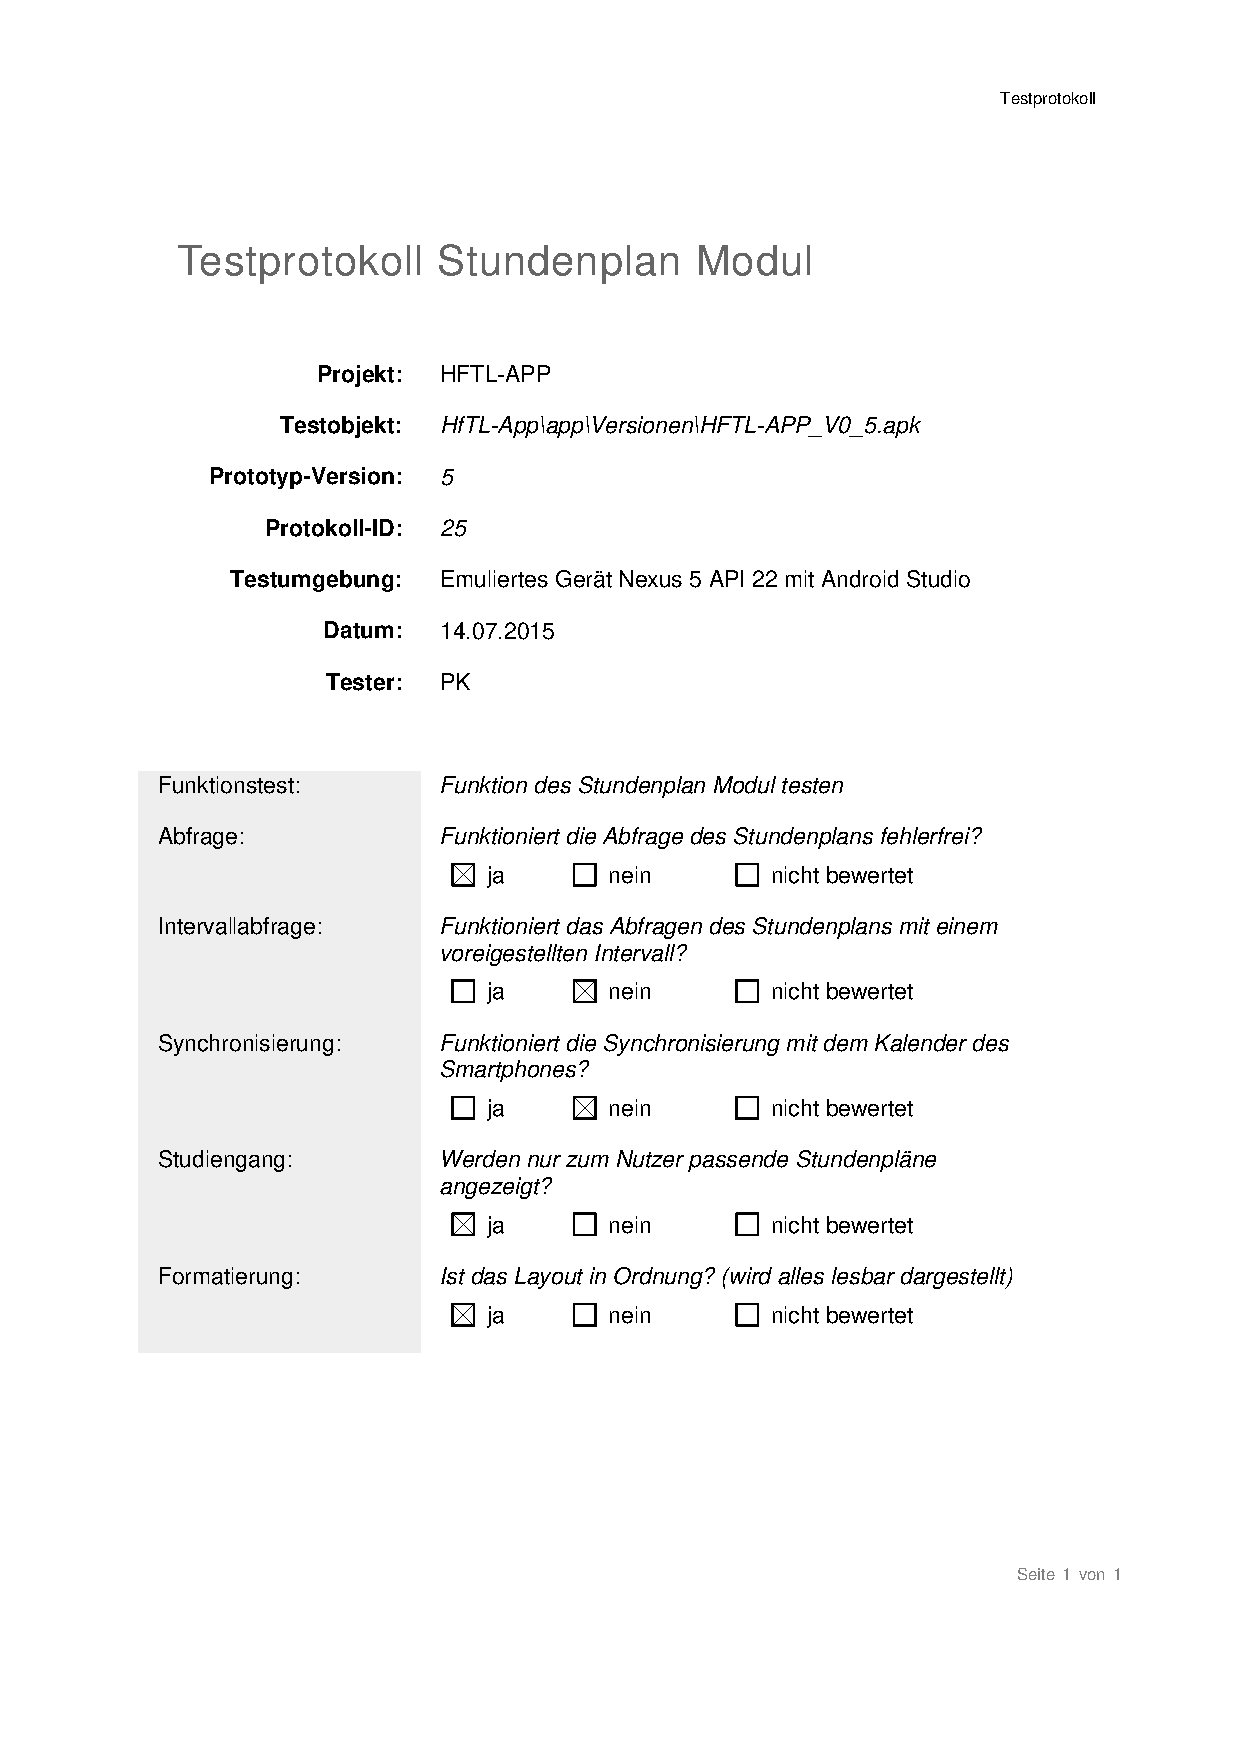
\includepdf[pages=-,noautoscale]{04_Anhang/files/Testprotokolle/Stundenplan_Modul/14072015_Testprotokoll_Stundenplan.pdf}

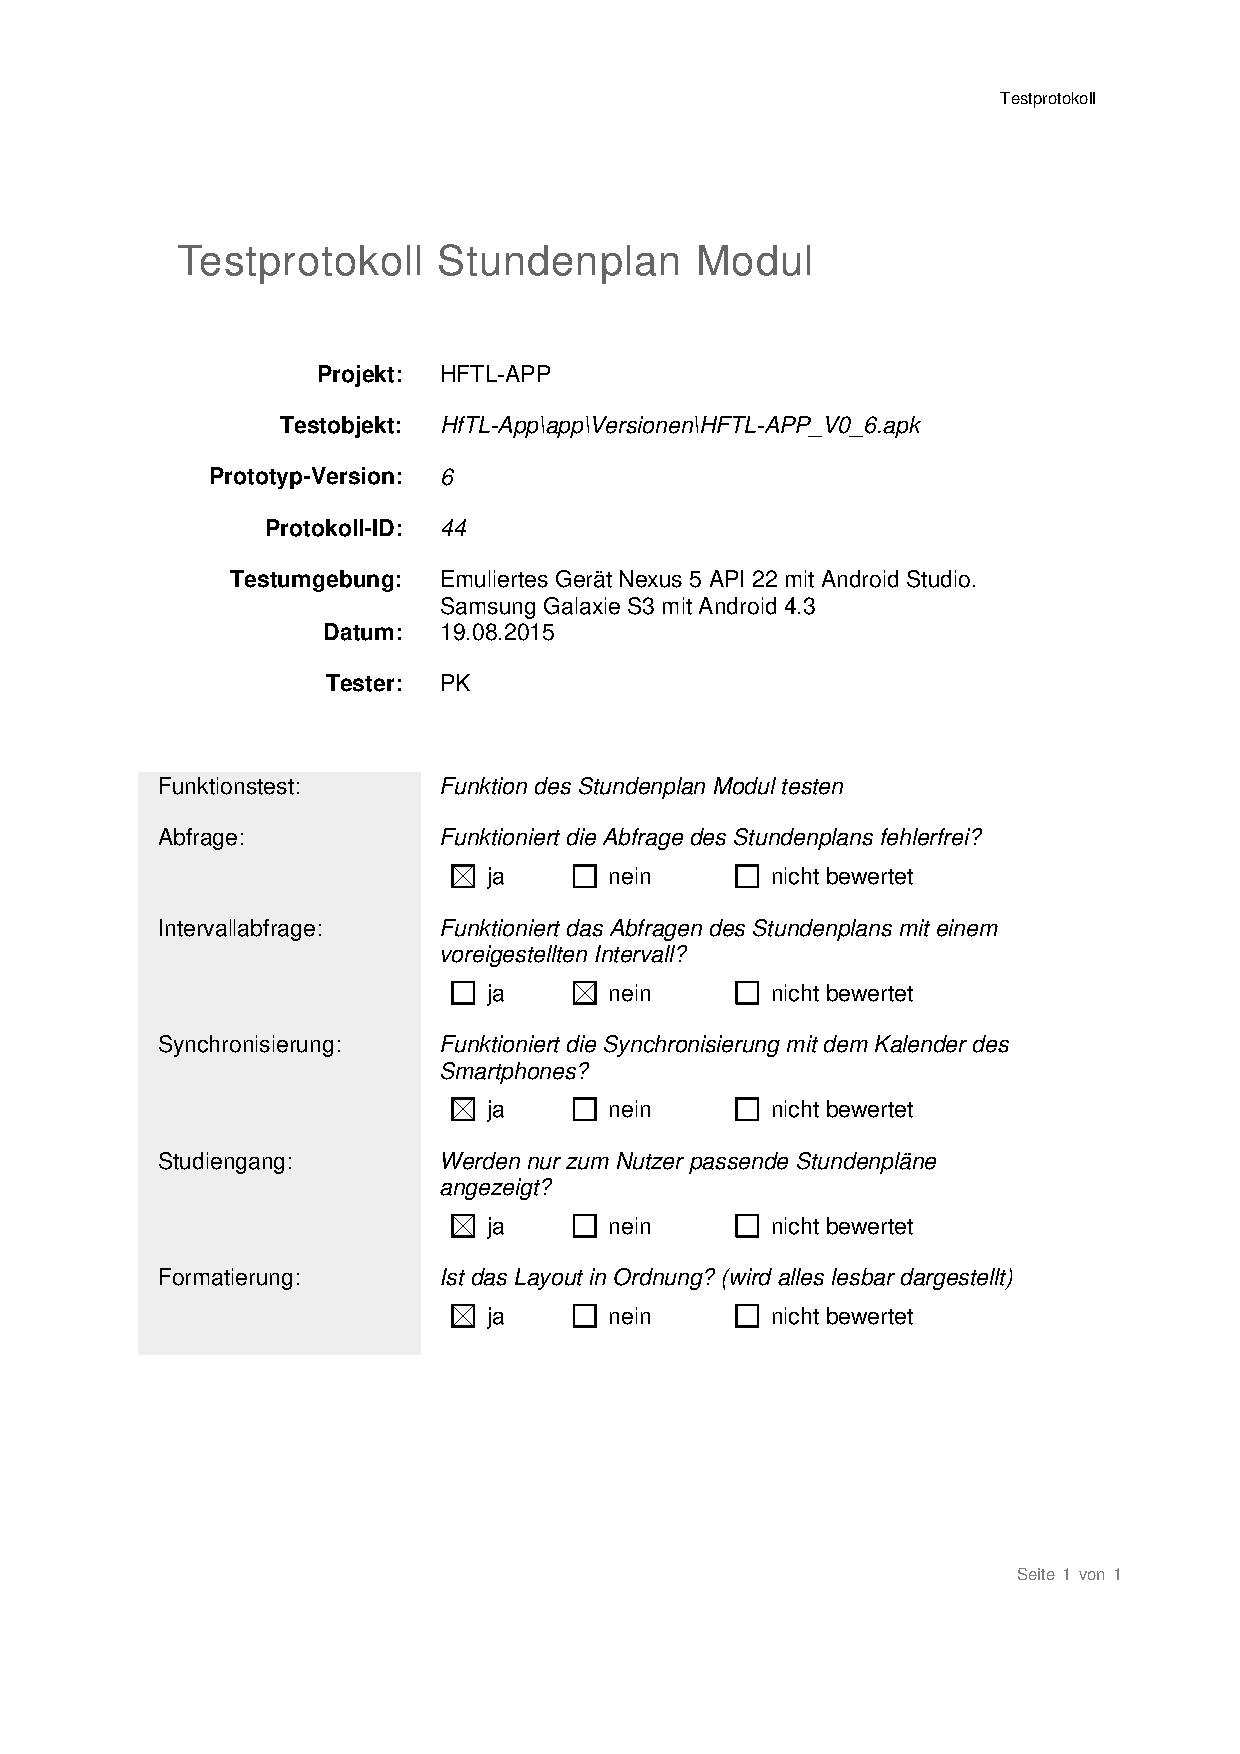
\includepdf[pages=-,noautoscale]{04_Anhang/files/Testprotokolle/Stundenplan_Modul/19082015_Testprotokoll_Stundenplan.pdf}

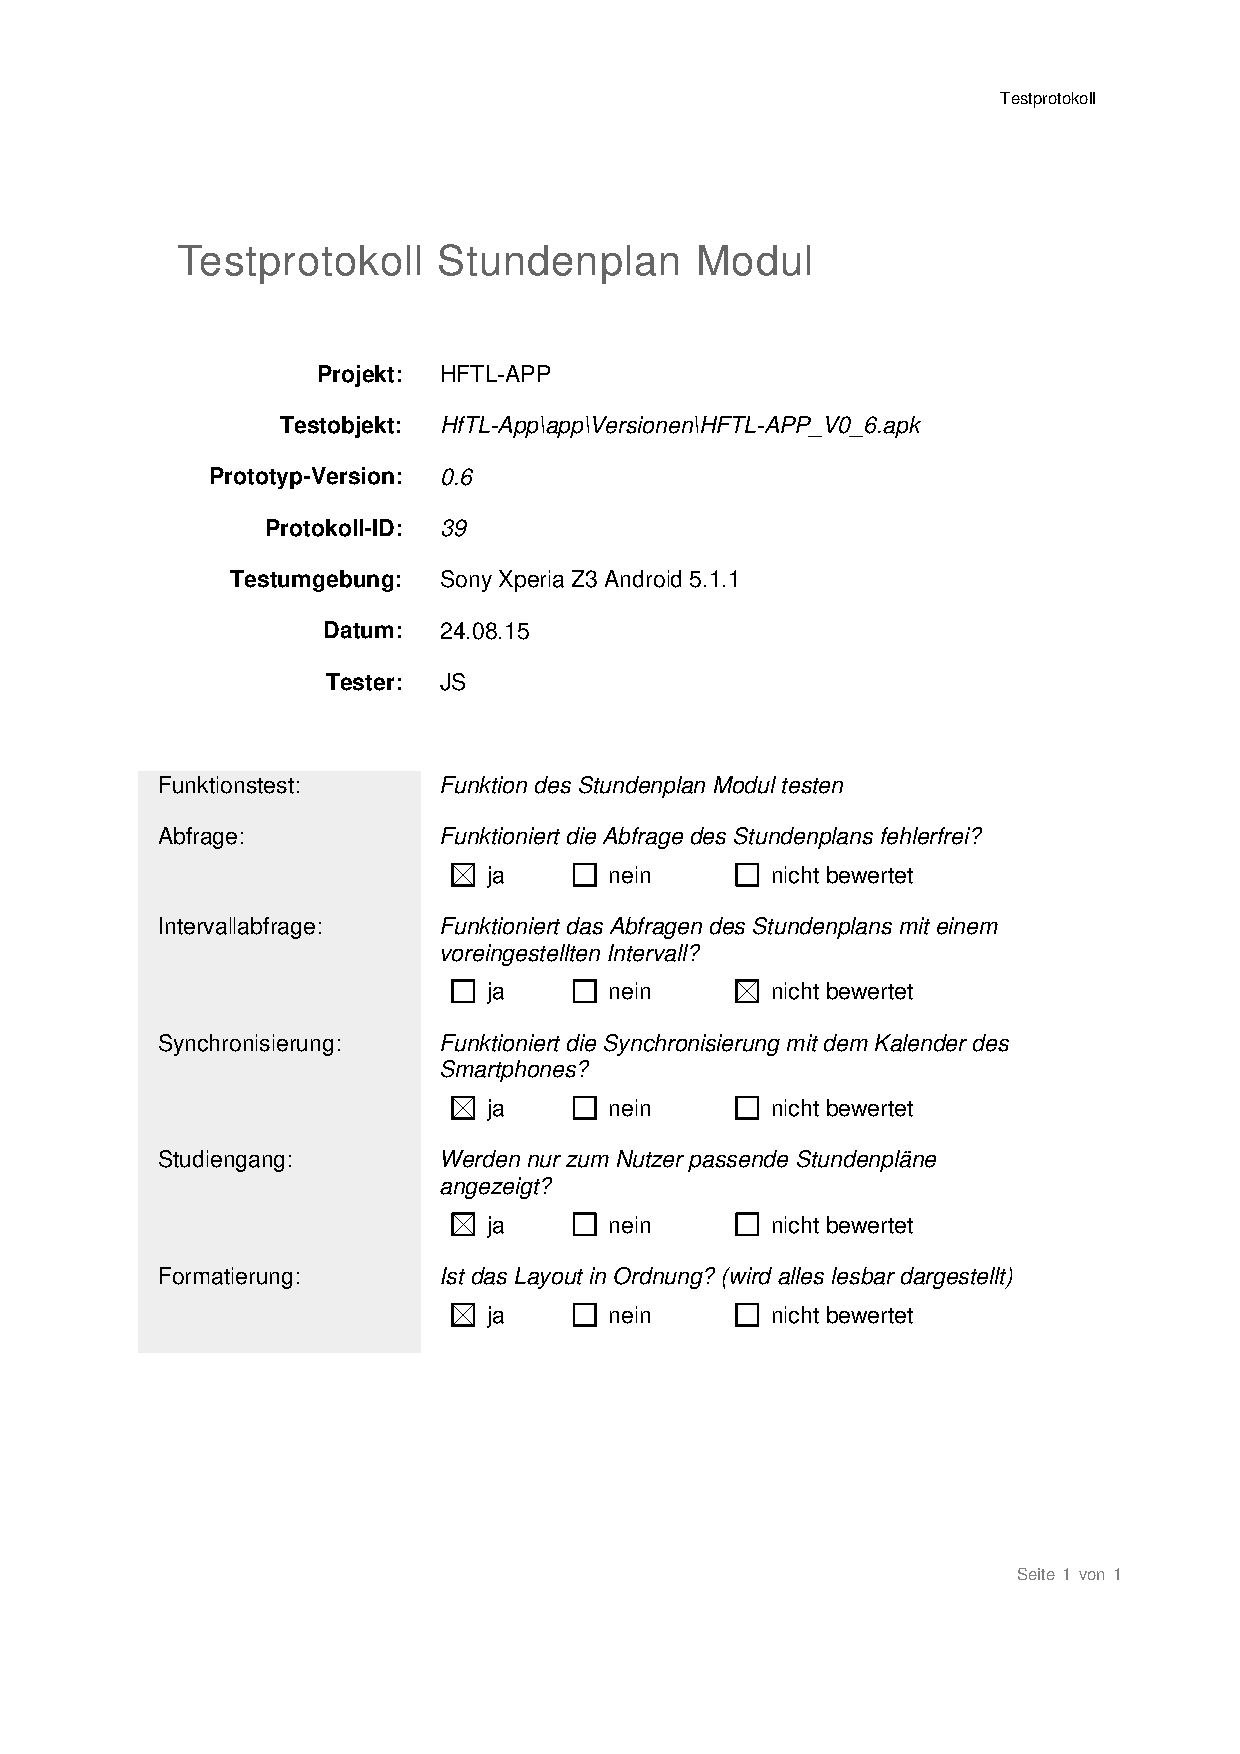
\includepdf[pages=-,noautoscale]{04_Anhang/files/Testprotokolle/Stundenplan_Modul/24082015_Testprotokoll_Stundenplan.pdf}






















\end{document}



